%%
%% Author: Dario Chinelli
%% from 2020-09-29 to 2021-04-13
%%

							% Preamble
\documentclass[11pt]{article}

							% Packages
\usepackage[top=1in, bottom=1in, left=1in, right=1in]{geometry}
\usepackage{amsmath}
\usepackage{enumitem}
\usepackage{amssymb}
\usepackage{tikz}
\usepackage{siunitx}
\usepackage{imakeidx}
\usepackage{graphicx}
\usepackage{subfig}
\graphicspath{ {img/} }
\usepackage{color}   %May be necessary if you want to color links
\usepackage{hyperref}
\hypersetup{
    colorlinks=true, %set true if you want colored links
    linktoc=all,     %set to all if you want both sections and subsections linked
    linkcolor=blue,  %choose some color if you want links to stand out
}

							% Document
\begin{document}

\title{\textbf{Appunti del corso di Struttura della Materia 1} \\
Laurea in Fisica - Università di Ferrara} 

\author{Scritto e impaginato in \LaTeX\ da \textbf{Dario Chinelli} nel 2021}

\date{aggiornato al 9 aprile 2021}

\maketitle

\newpage

\tableofcontents
							% inizio capitoli
% \iffalse
    \include{sections/Constants}

    %%
%% Author: dariochinelli
%% 2021-04-03
%%


\section{Il corpo nero}
Il corpo nero è un concetto utile per descrivere un oggetto le cui pareti si trovino a temperatura $T$ uniforme e costante, esso emette uno spettro di radiazione continuo che dipende solamente dalla temperatura e non dal materiale di cui è composto.
Le cariche elettriche costituenti le pareti si muovono in virtù dell'agitazione termica e così facendo irraggiano onde elettromagnetiche che vanno riempiendo la cavità: in questo modo si trasferisce energia dalle pareti al campo elettromagnetico al suo interno.
Tali onde elettromagnetiche a loro volta urtando contro le pareti trasferiscono energia dal campo elettromagnetico alle pareti.
Quando si raggiunge l'equilibrio termico tra le onde all'interno e le pareti dell'oggetto si ha che l'energia ricevuta è uguale a quella emessa.\\
\textbf{Definiamo} \\
\underline{\textit{Radianza Spettrale}}: $R_T(\nu)$ potenza su area, ovvero energia emessa per unità di tempo nell'intervallo di frequenze tra $\nu$ e $\nu+d\nu$ da un'area unitaria di superficie ad una certa temperatura $T$. \\
\underline{\textit{Radianza Totale} o \textit{Radianza}}: $R_T= \int_0^{\infty} R_T(\nu)d\nu$ integrale su tutte le frequenze della radianza spettrale, descrive l'energia totale per unità di tempo di un'area unitaria di superficie ad una certa temperatura $T$.
\begin{figure}[h]
\centering
\includegraphics[scale=0.6]{/Spectral_radiancy}
\caption{Radianza spettrale di corpo nero a tre diverse temperature. Notare come il picco si sposti all'aumentare della temperatura.}
\end{figure}
Per descrivere la radiazione di corpo nero Rayleigh e Jeans utilizzarono (anche) le seguenti leggi empiriche:
la \textbf{legge di Stefan-Boltzmann}:
\begin{equation}
R_T = \sigma T^4
\end{equation}
che descrive la radianza totale in funzione della temperatura ed in cui compare la 
\begin{equation}
\mbox{\underline{costante di Stefan-Boltzmann}} \quad \sigma = 5.67 \cdot 10^{-8} \frac{W}{m^2 \cdot K^4}
\end{equation}
La \textbf{legge di spostamento di Wien} afferma che la frequenza di picco è proporzionale alla temperatura
\begin{equation}
\begin{split}
& \nu_{max} \propto T \\
& \mbox{ed usando la seguente relazione} \quad \lambda\nu = c \\
& \lambda_{max}T = \SI{2.898e-3}{mK}
\end{split}
\end{equation}
L'oggetto reale più simile al concetto teorico di corpo nero è la \underline{cavità di corpo nero}, cioè un oggetto cavo con pareti metalliche avente un piccolo buco sulla superficie: la radiazione che esce dal foro è interpretabile come corpo nero, vedi figura.
\begin{figure}[h]
\centering
\includegraphics[scale=0.6]{/cavita_corponero}
\end{figure}
Introduciamo la \underline{\textbf{radiazione di cavità}} $\rho_T(\nu)$, che è la densità di energia contenuta in una unità di volume della cavità ad una certa temperatura $T$,
essa è ovviamente proporzionale alla Radianza totale, la cui derivazione è basata su ragionamenti puramente geometrici, in particolare la relazione è data da:
\begin{equation}
\frac{c}{4}\rho_T(\nu)=R_T(\nu)
\end{equation}


\subsection{Teoria classica di corpo nero di Rayleigh e Jeans}
A inizio '900 spiegare la forma dello spettro di corpo nero era uno dei problemi più dibattuti.
A dare un grande contributo furono Rayleigh e Jeans, che elaborarono la teoria classica di corpo nero, basandosi sulla fisica classica, per modellizzare la forma dello spettro di corpo nero.
Quindi si impegnarono nel trovare un modello teorico che potesse spiegare i risultati sperimentali. \\
Il ragionamento si divide in tre passaggi:
\begin{enumerate}[label=\Roman{*}.]
\item Le onde elettromagnetiche all'interno della cavità sono onde stazionarie?
\item Come contare il numero di onde stazionarie?
\item È possibile associare un'energia alle onde elettromagnetiche?
\end{enumerate}
\begin{figure}[h]
\centering
\includegraphics[scale=0.7]{/cubo_CorpoNero}
\caption{cubo Corpo Nero}
\end{figure}
Si consideri una cavità cubica e metallica riscaldata a temperatura $T$.
Essi ragionarono con le frequenze delle onde elettromagnetiche contenute nella cavità.
Vediamo in dettaglio i passaggi seguiti da Rayleigh e Jeans.
\begin{enumerate}[label=\Roman{*}.]
\item Prima di tutto occorre dimostrare che tali onde siano stazionarie.
Ogni onda può essere scomposta lungo le tre componenti spaziali e studiata indipendentemente. 
Consideriamo il lato del cubo $x \in (0, a)$.
La radiazione elettromagnetica è trasversale, cioè il campo elettrico $\vec{E}$ è perpendicolare alla direzione di propagazione dell'onda, dunque il campo è parallelo alla parete, ma ciò porta all'annullarsi di $\vec{E}$ sulla parete, perciò sui lati del cubo deve esserci ampiezza nulla, e quindi $0$ e $a$ sono due nodi.
Le onde sono dunque stazionarie.
\begin{figure}[h]
\centering
\includegraphics[scale=0.6]{/modiVibrazione}
\caption{modi vibrazione}
\end{figure}
\item Occorre contare il numero di onde, cominciamo dal caso 1-D lungo $x$
\begin{equation}
\begin{split}
& E(x, t) = E_0 \sin \Bigl(  \frac{2 \pi x}{\lambda}  \Bigr) \sin (2\pi \nu t) \\
& \frac{2x}{\lambda} = 0,1,2,3 ... = n \in \mathbb{N}
\end{split}
\end{equation}
Quindi $n=0$ corrisponde all'estremità, fissa, in $x=0$ e tutte le possibili onde stazionarie si trovano imponendo $x=a$:
\begin{equation}
\begin{split}
& \frac{ 2a}{\lambda } = n \quad\quad n = 1,2,3, ... \\
& \mbox{utilizzando la relazione} \quad \nu = \frac{c}{\lambda} \\
& \nu = \frac{ c n }{2a } \quad n = 1,2,3, ...
\end{split}
\end{equation}
Che sono quindi i valori permessi di frequenza per onde stazionarie.
\begin{figure}[h]
\centering
\includegraphics[scale=0.7]{/Blackbody_nodi}
\end{figure}
\begin{equation}
\begin{split}
& d = (\frac{ 2a}{c }) (\nu + d\nu) \quad - \quad d = (\frac{ 2a}{c }) \nu \\
& N(\nu)d\nu = 2 \Bigl(  \frac{2a}{c}  \Bigr) d\nu = \frac{4a}{c}d\nu 
\end{split}
\end{equation}
Nel caso unidimensionale questo è il numero di modi di vibrazione, dove il fattore 2 è dovuto al fatto che ci siano due possibili polarizzazioni $S$ e $P$. \\
\textbf{NB} Nel caso 1-D il numero di frequenze possibili non dipende da $\nu$.
Passiamo a 3 dimensioni, il valore di $n$ dipenderà ora da tre parametri $n_x, n_y, n_z \in \mathbb{N}$, da cui dipende anche il numero di frequenze permesse:
\begin{equation}
\begin{split}
& \frac{2a}{\lambda} = \sqrt{n_x^2 + n_y^2 + n_z^2} \\
& \nu = \frac{ c}{\lambda } = \frac{ c}{2a } \sqrt{n_x^2 + n_y^2 + n_z^2}
\end{split}
\end{equation}
\begin{figure}[h]
\centering
\includegraphics[scale=0.6]{/sfrera_nodi_permessi}
\caption{Numero di punti tra due shell a distanza $dr$, associati alle frequenze permesse}
\end{figure}
Conto quindi il numero di frequenze dal raggio $r$ al raggio $r + dr$:
\begin{equation}
\begin{split}
& N(\nu) d\nu = N(r)dr \\ 
& r = \frac{2a}{c}\nu \\
\end{split}
\end{equation}
ma il numero di punti nel volume dal raggio $r$ al raggio $r + dr$ è proprio il volume stesso, nel conto seguente utilizzo la sostituzione per $r$ appena trovata:
\begin{equation}
\begin{split}
& N(r) dr = \frac{ 1}{8 } 4 \pi r^2 dr = \frac{ \pi r^2 dr}{2 } \\
& N(\nu)d\nu = \frac{ \pi}{2 } \Bigl(  \frac{ 2a}{c }  \Bigr)^3 \nu^2 d\nu \\
& \mbox{che moltiplico x2 perché ho due stati di polarizzazione} \\
\Rightarrow & N(\nu) d\nu = \frac{ 8\pi V}{c^3 } \nu^2 d\nu
\end{split}
\end{equation}
ottengo così \underline{il numero di frequenze permesse} (modi di vibrazione) per le onde elettromagnetiche stazionarie all'interno della cavità di corpo nero, dove $V=a^3$ è il volume della cavità. \\
\textbf{NB} Nel caso 3-D il numero di frequenze possibili dipende da $\nu$.
\item Stima dell'energia media di ogni onda stazionaria di frequenza $\nu$.
Se ho un sistema di particelle in equilibrio termico, l'energia cinetica media per molecola per grado di libertà è data dalla \textbf{legge di equipartizione dell'energia}:
\begin{equation}
\begin{split}
\bar \varepsilon = \frac{ 1}{2 } & k_B T \\
\mbox{costante di Boltzmann } & k_B = \SI{1.3806e-23}{J/K}
\end{split}
\end{equation}
Considerando le onde come oggetti oscillanti devo tenere in considerazione anche l'energia potenziale, con argomentazioni di fisica classica, trovo l'energia media totale:
\begin{equation}
\bar \varepsilon = k_B T
\end{equation}
\end{enumerate}

\paragraph{Formula classica di Rayleigh Jeans per il corpo nero}
Moltiplicando il numero di onde stazionarie all'interno della cavità 
$$\frac{8 \pi \nu^2}{c^3}$$
per l'energia media di ogni onda stazionaria
$$k_BT$$
e dividendo per il volume $V$ si ottiene la \underline{densità di energia} $\rho_T(\nu)$ all'interno della cavità di corpo nero
\begin{equation}
\rho_T(\nu)d\nu = \frac{8 \pi \nu^2 k_B T }{c^3}d\nu
\end{equation}
La teoria classica di corpo nero è verificata solo per valori piccoli di $\nu$ e si discosta rapidamente dai dati sperimentali al crescere della frequenza, vedi figura \ref{catastrofeUV}.
\begin{figure}[h]
\centering
\includegraphics[scale=0.6]{/catastrofe_ultravioletta}
\caption{Catastrofe ultravioletta}
\label{catastrofeUV}
\end{figure}


\subsection{Statistica classica di Boltzmann}
Introduciamo la legge statistica classica di Boltzmann (o di Maxwell-Boltzmann) come la probabilità $P$ di trovare una certa entità di un sistema con energia nell'intervallo tra $\varepsilon$ e $\varepsilon+d\varepsilon$, data dalla formula
\begin{equation}
P(\varepsilon)d\varepsilon = C e^{ -\frac{\varepsilon}{k_BT } }
\end{equation}
Tale formula è valida quando il numero degli stati di energia \underline{non} dipende da $\varepsilon$, valida quindi ad esempio per l'oscillatore armonico unidimensionale.
La costante $C$ si calcola imponendo che l'integrale su tutto lo spettro di energie sia pari a $1$:
\begin{equation}
\begin{split}
\int_{0}^{\infty} P(\varepsilon) d\varepsilon & = C \int_{0}^{\infty} e^{ -\frac{\varepsilon}{k_BT } } d\varepsilon = 1 \\
C & = \frac{ 1}{k_BT }
\end{split}
\end{equation}
Per cui si trova la formula che descrive la statistica classica di Boltzmann 
\begin{equation}
P(\varepsilon) = \frac{ e^{ - \frac{\varepsilon}{k_BT } } }{k_BT }
\end{equation}

\paragraph{Applico la statistica di Boltzmann} agli elementi del set di onde stazionarie oscillanti nella cavità di corpo nero, quindi l'energia media è data da: 
a numeratore l'energia $\varepsilon$ moltiplicata (pesata) per la probabilità che l'entità abbia quell'energia (integrata su tutti i valori di energia), a denominatore ho la probabilità di trovare l'entità con qualsiasi energia (integrata su tutti i valori di energia), ponendo $\beta=\frac{1}{k_BT}$
\begin{equation}
\begin{split}
\bar\varepsilon & =\frac{\int_{0}^{\infty} \varepsilon P(\varepsilon)\,d\varepsilon}{\int_{0}^{\infty} P(\varepsilon)\,d\varepsilon} 
= \frac{\int_{0}^{\infty} \varepsilon \frac{ e^{ - \frac{\varepsilon}{k_BT } } }{k_BT } d\varepsilon}{\int_{0}^{\infty} \frac{ e^{ - \frac{\varepsilon}{k_BT } } }{k_BT }d\varepsilon}
= \frac{\int_{0}^{\infty} \varepsilon \beta e^{ - \beta \varepsilon } d\varepsilon}{\int_{0}^{\infty} \beta e^{ - \beta \varepsilon } d\varepsilon} \\
& = \frac{\int_{0}^{\infty} \varepsilon e^{ - \beta \varepsilon } d\varepsilon}{\int_{0}^{\infty} e^{ - \beta \varepsilon } d\varepsilon}
= - \frac{ d}{d\beta } \Bigl[  \ln \Bigl(  \int_0^{\infty} e^{ -\beta \varepsilon } d\varepsilon  \Bigr)   \Bigr]
= - \frac{ d}{d\beta } \Bigl(  \ln \frac{ 1}{\beta }  \Bigr) \\
& = \beta \frac{ 1}{\beta^2 } 
= \frac{ 1}{\beta } 
= k_BT
\end{split}
\label{energia_media_blackbody}
\end{equation}
Ottenendo così l'energia media di ogni onda stazionaria 
\begin{equation}
\bar \varepsilon = k_B T
\end{equation}
uguale al valore utilizzato da Rayleigh e Jeans e per cui si ha la catastrofe ultravioletta.


\subsection{Ipotesi quantica di Planck e formula di Planck per il corpo nero}
Planck ipotizza che l'energia non possa assumere qualsiasi valore ma solo valori discreti
$$\varepsilon = 0,\Delta\varepsilon,2\Delta\varepsilon,3\Delta\varepsilon, ...$$
Allora per misurare l'area del sottografico, e quindi la Radianza totale, non occorrerà più eseguire un integrale ma piuttosto una sommatoria su tutti i "rettangolini" discreti.
\begin{figure}[h]
    \centering
    \subfloat[Ipotesi quantica di Planck]{
        \label{ipotesi_quantica_Planck}
        \includegraphics[width=0.5\textwidth]{/ipotesi_quantica_Planck}
    }
    \subfloat[Sommatoria sui rettangolini del sottografico]{
        \label{rettangolini}
        \includegraphics[width=0.5\textwidth]{/rettangolini}
    }
%    \caption{Overall_caption}
    \label{ipotesi_quantica_Planck_rettangolini}
\end{figure}
Analizzando l'andamento di $\bar\varepsilon$ in funzione di $\Delta\varepsilon$ si trova l'espressione:
\begin{equation}
\bar\varepsilon = \frac{ \Delta\varepsilon}{e^{ \frac{ \Delta\varepsilon}{k_BT } } - 1 }
\end{equation}
per cui i limiti di tale espressione sono
\begin{equation}
\begin{split}
& se \quad \Delta\varepsilon \rightarrow 0 \quad \Rightarrow \quad \bar\varepsilon \sim \frac{ 2 k_B^2 T^2 }{2kT + \Delta\varepsilon } \rightarrow k_BT  \quad \mbox{dove } e^x \sim 1 + x + \frac{ x^2}{2 } \\
& se \quad \Delta\varepsilon = k_BT \quad \Rightarrow \quad \bar\varepsilon = \frac{ k_BT }{ e - 1 } < k_BT \\
& se \quad \Delta\varepsilon \rightarrow \infty \quad \Rightarrow \quad \bar\varepsilon = \lim_{\Delta\varepsilon = \infty}  \frac{ \Delta\varepsilon}{e^{ \frac{ \Delta\varepsilon}{k_BT } } - 1 } = 0
\end{split}
\end{equation}
Quindi il risultato classico $\bar\varepsilon = k_BT$ è utile solo per $\Delta\varepsilon = h\nu \rightarrow 0$ ovvero per frequenze $\nu$ piccole.
La soluzione si trova se si mettono in correlazione $\Delta\varepsilon \propto \nu$ quindi scrivendo $\Delta\varepsilon = h\nu$ dove $h=\SI{6.63e-34}{J.s}$ è la Costante di Planck.
La \underline{quantizzazione dell'energia}, quindi i valori possibili dell'energia, si scrive come $n h \nu$ con $n = 0,1,2, ...$
L'espressione della probabilità $P(\varepsilon)$ è la legge statistica classica di Boltzmann in cui si sostituisce la relazione dell'energia $\varepsilon$ di Planck
\begin{equation}
\begin{split}
& P(\varepsilon) = \frac{ e^{ -\frac{ \varepsilon}{ k_BT} }}{k_BT }  \quad\quad \varepsilon= n h\nu \\
\bar\varepsilon & = \frac{ \sum_{n=0}^{\infty} \varepsilon P(\varepsilon)}{\sum_{n=0}^{\infty} P(\varepsilon) }
= \frac{ \sum_{n=0}^{\infty}  \frac{ nh\nu}{k_BT } e^{ -\frac{ nh\nu}{k_BT } }  }{\sum_{n=0}^{\infty} \frac{ 1 }{k_BT } e^{ -\frac{ nh\nu}{k_BT } } } \\
& = k_BT \frac{\sum_{n=0}^{\infty} n\alpha e^{ -n\alpha } }{\sum_{n=0}^{\infty} e^{ -n\alpha } } \quad\quad \alpha = \frac{ h\nu}{k_BT }
\end{split}
\end{equation}
si procede nel calcolo come nel caso classico, introducendo la seguente catena di uguaglianze
\begin{equation}
- \alpha \frac{ d}{d\alpha } \ln \sum_{n=0}^{\infty} e^{-n\alpha} = \frac{ - \alpha \frac{ d}{d\alpha } \sum_{0}^{\infty} e^{-n\alpha} }{ \sum_{0}^{\infty} e^{-n\alpha}} = 
\frac{ - \sum_{0}^{\infty} \alpha \frac{ d}{d\alpha } e^{-n\alpha} }{ \sum_{0}^{\infty} e^{-n\alpha}} = \frac{\sum_{0}^{\infty} n\alpha e^{ -n\alpha } }{\sum_{0}^{\infty} e^{ -n\alpha } }
\end{equation}
sostituendo si ottiene
\begin{equation}
\begin{split}
\bar\varepsilon = k_BT \Bigl(  - \alpha \frac{ d}{d\alpha } \ln \sum_{n=0}^{\infty} e^{ -n\alpha }  \Bigr) = -h\nu \frac{ d}{d\alpha } \ln \sum_{n=0}^{\infty} e^{ -n\alpha }
\end{split}
\end{equation}
utilizziamo ora la serie geometrica per eseguire la derivata
\begin{equation}
\sum_{n=0}^{\infty} e^{ -n\alpha } = 1 + e^{ -\alpha } + e^{ -2\alpha } + ... = 1 + x + x^2 + ... = \frac{ 1}{1-x } = \frac{ 1}{1- e^{- \alpha } }
\end{equation}
e si scrive il risultato come
\begin{equation}
\bar\varepsilon = - h\nu \Bigl[ - \frac{ e^{ -\alpha }}{1 - e^{ -\alpha } } \Bigr] = \frac{ h\nu}{ e^{ \alpha } - 1 } = \frac{ h\nu}{ e^{ \frac{ h\nu}{k_BT } } - 1} 
\end{equation}
quindi l'espressione finale dell'\textbf{energia media delle onde nella cavità} è
\begin{equation}
\bar\varepsilon = \frac{ h\nu}{ e^{ \frac{ h\nu}{k_BT }} - 1} 
\end{equation}
Per ottenere l'espressione della \underline{radiazione di cavità} moltiplico il numero di modi di vibrazione possibili per un'onda stazionaria all'interno della cavità
$$\frac{ 8\pi\nu^2}{c^3 }$$
per l'espressione dell'energia media di ogni onda stazionaria nella nuova ipotesi di Planck, ottengo quindi
\begin{equation}
\rho_T(\nu) d\nu = \frac{ 8\pi\nu^2}{c^3 } \frac{ h\nu}{ e^{ \frac{ h\nu}{k_BT }} - 1} d\nu
\end{equation}
anche detta \textbf{Formula di Planck per il corpo nero (1900)}, tale formula è in perfetto accordo con i dati sperimentali.
Questo risultato da inizio alla fisica moderna, introducendo il concetto di energia quantizzata inizia quindi la meccanica quantistica.
Cerchiamo ora un'espressione analoga in funzione di$\lambda$
$$\rho_T(\lambda) d\lambda = -\rho_T(\nu)d\nu $$
considero che
$$\nu = \frac{ c}{\lambda } \quad \Rightarrow \quad d\nu = -\Bigl(  \frac{ c}{\lambda^2 }  \Bigr) d\lambda \quad \Rightarrow \quad \frac{ d\nu}{d\lambda } = -\Bigl(  \frac{ c}{\lambda^2 }  \Bigr) $$
quindi sostituendo in questo modo
$$\rho_T(\lambda) = -\rho_T(\nu) \frac{ d\nu}{d\lambda } = -\rho_T(\nu) \frac{ c}{\lambda^2 }$$
si ottiene l'espressione cercata
\begin{equation}
-\rho_T(\lambda) d\lambda = \frac{ 8\pi h c }{\lambda^5 } \frac{ d\lambda}{e^{ \frac{ hc}{\lambda k_B T } } -1 }
\end{equation}
\begin{figure}[h]
\centering
\includegraphics[scale=0.6]{/spettri_corponero}
\caption{Vari spettri di corpo nero}
\end{figure}

\paragraph{Postulato di Planck:} \textit{ogni entità fisica con un grado di libertà la cui "coordinata" è una funzione sinusoidale del tempo può avere solo energia totale $E$ tale che sia soddisfatta la relazione \\
$\varepsilon = n h \nu$ con $n=0,1,2, ...$ naturale.} \\
Il postulato di Planck si estende quindi a tutte le entità fisiche modellizzabili come oscillatori armonici semplici.
\begin{figure}[h]
\centering
\includegraphics[scale=0.6]{/energia_quantizzata}
\caption{Confronto grafico tra la trattazione classica e quella quantizzata proposta da Planck}
\end{figure} 

\paragraph{Derivazione della legge di Stefan-Boltzmann}
Come si arriva alla formula di Stefan-Boltzmann partendo dalla formula di Planck per il corpo nero?
Ricordo che esiste le relazioni
$$\frac{ c}{4 } \rho_T(\nu) = R_T(\nu) \quad e \quad R_T = \int_0^{\infty} R_T(\nu)d\nu$$
quindi
\begin{equation}
\begin{split}
\rho_T(\nu) d\nu & = \frac{ 8\pi\nu^2}{c^3 } \frac{ h\nu}{ e^{ \frac{ h\nu}{k_BT }} - 1} d\nu \\
R_T &= \int_0^{\infty} \frac{ 2\pi h}{c^2 } \frac{ \nu^3}{e^{ \frac{ h\nu}{k_BT } } - 1 } d\nu \\
& = \frac{ 2\pi h}{c^2 } \Bigl(  \frac{ k_BT}{h }  \Bigr)^4 \int_0^{\infty} \frac{ x^3}{e^x - 1 }dx \quad \mbox{dove} \quad x=\frac{ h\nu}{k_BT }\\
\end{split}
\end{equation}
calcolo l'integrale noto
\begin{equation}
\int_0^{\infty} \frac{ x^3}{e^x - 1 }dx = \frac{ \pi^4}{15 }
\end{equation}
da cui ottengo il risultato finale 
\begin{equation}
R_T = \sigma T^4
\end{equation}
in cui compare la costante di Stefan Boltzmann
\begin{equation}
\sigma = \frac{ 2\pi^5 k_B^4}{15 h^3 c^2 } \simeq \SI{5.676e-8}{W / m^2 K^4}
\end{equation}

\newpage

\paragraph{Esercizio}
Si consideri una massa puntiforme $m=\SI{0.01}{kg}$ appesa ad un filo di lunghezza $l=\SI{0.1}{m}$ e sia $\theta=\SI{0.1}{rad}$ l'angolo massimo di oscillazione. L'energia di questo pendolo appare continua o quantizzata? \\
\underline{Soluzione:}
utilizzando risultati di fisica classica, calcolo la frequenza di questo pendolo
\begin{equation}
\nu = \frac{ 1}{2\pi } \sqrt{\frac{ g}{l }} = \frac{ 1}{2\pi }\sqrt{\frac{ \SI{9.81}{m/s^2}}{\SI{0.1}{m} }} = \SI{1.6}{Hz}
\end{equation}
e calcolo l'energia potenziale del pendolo
\begin{equation}
mgh = mgl(1-\cos \theta) = \SI{0.01}{kg} \cdot \SI{9.81}{m/s^2} \cdot \SI{0.1}{m} \cdot (1-\cos \theta) = \SI{5e-5}{j}
\end{equation}
Il quanto di energia che posso associare a questo pendolo 
\begin{equation}
\Delta E = h\nu = \SI{6.63e-34}{j.s} \cdot \SI{1.6}{Hz} = \SI{e-33}{j}
\end{equation}
nell'ipotesi che l'energia del pendolo sia quantizzata.
Ottengo un numero molto piccolo rispetto all'energia complessiva del pendolo, per cui il rapporto
\begin{equation}
\frac{ \Delta E }{E } = \SI{2e-29}{}
\end{equation}
Possiamo renderci conto della quantizzazione solo quando il quanto $\Delta E$ e l'energia $E$ sono grandezze confrontabili.
Da cui si vede come la fisica classica offra un'ottima approssimazione per lo studio di problemi di questo tipo.




    %%
%% Author: dariochinelli
%% 2021-04-05
%%


\section{Effetto fotoelettrico}
L'effetto fotoelettrico è uno dei possibili processi di interazione tra radiazione elettromagnetica e materia, come anche l'effetto Compton.
La radiazione elettromagnetica non si manifesta solo nella natura ondulatoria ma anche nella natura particellare, l'effetto fotoelettrico si spiega grazie all'interpretazione particellare.

\paragraph{Esperimenti di Hertz}
Nel 1887 Hertz, studiando la scarica dei conduttori elettrizzati stimolata da una scintilla elettrica nelle vicinanze,
si accorse che tale fenomeno è più intenso se gli elettrodi vengono illuminati con luce ultravioletta.

\subsection{Esperimento di Lenard (1900)}
La \underline{scoperta} dell'effetto fotoelettrico viene attribuita a Lenard.
Scopre che il motivo dell'osservazione di Hertz è che degli elettroni vengono emessi dal catodo (elettrodo negativo) quando si fa incidere su di esso della radiazione elettromagnetica, in particolare gli esperimenti erano fatti con luce visibile e ultravioletta.

\paragraph{Apparato sperimentale:} 
Consiste in un tubo di vetro sotto vuoto che contiene due elettrodi a cui viene applicata una differenza di potenziale.
Della luce ultravioletta viene fatta incidere su un elettrodo (negativo) da cui fuoriescono elettroni (fotoelettroni) attirati verso l'elettrodo positivo a causa della d.d.p. .
L'emissione di elettroni viene rilevata come una corrente misurata con un amperometro.
Vedi figura \ref{Schema_EffettoFotoelettrico} per un'illustrazione grafica dell'apparato.
\begin{figure}[h]
\centering
\includegraphics[scale=0.5]{/Schema_EffettoFotoelettrico}
\caption{Schema dell'esperimento di Lenard del 1900}
\label{Schema_EffettoFotoelettrico}
\end{figure}

\paragraph{Risultati sperimentali}
\underline{il primo risultato sperimentale} è la corrente misurata in funzione del potenziale applicato (vedi grafico a sinistra in figura \ref{risultati_Lenard}).
Fissata l'intensità della luce incidente al valore $I_a$, quando il potenziale che applico è elevato la corrente raggiunge un livello di saturazione, riesco a raccogliere quindi tutti i fotoelettroni uscenti dal catodo.
Se porto a zero il potenziale la corrente non si annulla e nemmeno se applico un potenziale negativo. 
Significa che i fotoelettroni emessi hanno una certa energia cinetica e anche invertendo la polarità dei due elettrodi, pur venendo in parte respinti, sono ancora in grado di raggiungere il catodo.
La \textit{fotocorrente} arriva a zero quando il potenziale applicato raggiunge il valore detto \textit{potenziale di stop} $V_0$.
\begin{figure}[h]
\centering
\includegraphics[scale=0.2]{/effetto_fotoelettrico}
\caption{Risultati esperimento}
\label{risultati_Lenard}
\end{figure}

L'energia cinetica massima dei fotoelettroni emessi dall'elettrodo è
\begin{equation}
K_{max} = e V_0
\end{equation}
Se considero una luce incidente con un'intensità massima $I_b$ (vedi grafico a sinistra in figura \ref{risultati_Lenard}), che si riferisce ad un'intensità minore rispetto alla precedente $I_a$, trovo un livello di saturazione minore rispetto al caso precedente ma vedo che il valore $V_0$ non cambia: l'energia cinetica massima degli elettroni non cambia, risulta essere indipendente dall'intensità della luce.
\underline{Il secondo risultato sperimentale} trovato (grazie al contributo di Millican, vedi grafico a destra in figura \ref{risultati_Lenard}) è che se plotto il potenziale di stop in funzione della frequenza della radiazione incidente trovo una relazione lineare, ma al di sotto di un certo valore di frequenza $\nu_0$, che prende il nome di \textit{frequenza di cutoff}, non osservo più l'effetto fotoelettrico: ovvero non osservo più l'emissione di elettroni dall'elettrodo colpito dalla radiazione.
% elenco
La fisica classica, con la teoria ondulatoria della luce, non è in grado di spiegare tre aspetti fondamentali di questo fenomeno:
\begin{enumerate}[label=\Roman{*}]
\item Poiché l'intensità della luce è proporzionale all'ampiezza del vettore campo elettrico al quadrato, il campo elettrico $\vec E$ dovrebbe aumentare all'aumentare dell'intensità della luce.
La forza applicata all'elettrone dovrebbe essere proporzionale al vettore campo elettrico e con esso l'energia cinetica degli elettroni dovrebbe aumentare, ma questo non accade: non si vede una dipendenza dell'energia cinetica dell'elettrone dall'intensità della luce incidente.
\item Esiste una frequenza di cutoff, e non si spiega il perché. Per la teoria ondulatoria se la luce è abbastanza intensa e fornisce abbastanza energia l'effetto fotoelettrico dovrebbe verificarsi per qualsiasi frequenza, ma non è così. 
\item Considerando una luce incidente molto debole, l'elettrone dovrebbe aver bisogno di un certo tempo per accumulare sufficiente energia per essere emesso, dovrebbe esserci un tempo misurabile in cui questo avviene.
Eppure non si misura nessun ritardo fra il momento in cui la luce incide sull'elettrodo e l'emissione dell'elettrone, l'esperimento sembra suggerire che il fenomeno avvenga istantaneamente.
\end{enumerate}

\subsection{Spiegazione dell'effetto fotoelettrico di Einstein}
La radiazione elettromagnetica è costituita da un insieme di pacchetti di energia: i \textit{fotoni}, denominati così dal chimico Lewis, di energia espressa da
\begin{equation}
E = h \nu
\end{equation}
dove $h$ è la costante di Planck e $\nu$ è la frequenza della radiazione.

\paragraph{Che differenza c'è rispetto a Planck?}
Planck aveva applicato la quantizzazione dell'energia agli elettroni accelerati sulle pareti di cavità, poi pensava che la radiazione si propagasse come onde di energia quantizzata, ma onde.
Einstein propone che l'energia che si irradia venga scambiata in pacchetti di quantità $h\nu$ che rimangono tali anche successivamente allo scambio.
(Se pensiamo al corpo nero: scambiata tra pareti e onde nella cavità).
Egli non contesta che la luce possa essere descritta in termini ondulatori, sottolinea però la natura corpuscolare della radiazione in fenomeni in cui la radiazione viene emessa e assorbita.
\begin{equation}
\begin{split}
Planck \quad & \Rightarrow \quad \mbox{onde di energia quantizzata} \\
Einstein \quad & \Rightarrow \quad \mbox{pacchetti di energia quantizzata} 
\end{split}
\end{equation}
L'effetto fotoelettrico per Einstein consiste nel completo assorbimento di un fotone da parte di un elettrone del catodo, che viene appunto fotoemesso.
La spiegazione matematica è la seguente
\begin{equation}
K = h\nu - W
\end{equation}
dove l'energia cinetica dell'elettrone emesso $K$ equivale alla differenza fra l'energia del fotone $h\nu$ completamente assorbito e una quantità $W$ che è il lavoro richiesto per strappare l'elettrone dal metallo.
L'energia cinetica massima è descritta dalla legge di Einstein per l'effetto fotoelettrico
\begin{equation}
K_{max} = h\nu - W_0
\end{equation}
Dove $W_0$ prende il nome di \textit{funzione lavoro} ed è una caratteristica del metallo utilizzato e corrisponde all'energia minima dell'elettrone per uscire dal catodo.

\paragraph{Potenziale di stop}
Dalla formula di Einstein si ricava il potenziale di stop:
\begin{equation}
\begin{split}
K_{max} = e & V_0 = h\nu - W_0 \\
& V_0 = \frac{ h\nu}{e } - \frac{ W_0}{e }
\end{split}
\end{equation}
quindi permette di comprendere meglio la relazione lineare tra il potenziale  di stop e la frequenza, vista in figura \ref{risultati_Lenard}.
La pendenza di tale curva è $\frac{ h}{e }$ e l'intercetta all'asse delle ordinate è $\frac{ W_0}{e }$; da questo studio è anche possibile ricavare la costante di Planck, come fece Millican trovando un valore molto vicino a quello che oggi riteniamo esatto.

\newpage

\paragraph{L'interpretazione di Einstein} ci mette nella condizione di poter rispondere ai quesiti posti in precedenza dalla fisica classica:
\begin{enumerate}[label=\Roman{*}]
\item "$K_{max}$ non dipende dall'intensità della luce" \\
Raddoppiare l'intensità della luce incidente, mantenendo la stessa frequenza, significa raddoppiare il numero di fotoni, ma il valore dell'energia di ogni fotone $h\nu$ rimane invariato e, appunto, $K_{max}$ non dipende dall'intensità della luce.
\item "Esistenza della frequenza di cutoff"\\
Se $K_{max} = 0 \quad \Rightarrow \quad h\nu_0 = W_0$ viene strappato un elettrone ma senza energia cinetica ed è quindi il limite per il verificarsi dell'effetto fotoelettrico, $\nu_0$ è la frequenza di cutoff.
\item "Non c'è un tempo di interazione"\\
L'energia è fornita in pacchetti concentrati di energia e quindi quando un fotone viene assorbito è assorbito tutto in una volta ed immediatamente si ha l'emissione di un elettrone.
\end{enumerate}
\textbf{NB:} l'effetto fotoelettrico, quindi un completo assorbimento del fotone incidente, può avvenire anche con fotoni di più alta energia del visibile (e.g. raggi X), che però andrà ad estrarre gli elettroni più legati al nucleo.


\subsection{Raffigurazione dello spettro elettromagnetico}
\begin{figure}[h]
\centering
\includegraphics[scale=0.6]{/spettro_elettromagnetico}
\caption{Spettro elettromagnetico}
\end{figure}






    \include{sections/EffettoCompton}

    %%
%% Author: dariochinelli
%% 2021-04-05
%%


\section{Diffrazione raggi X}
Nel 1913 Bragg scoprì che i solidi cristallini producono pattern molto particolari nella diffrazione di raggi $X$.
Scoprì infatti che i cristalli, a determinate lunghezze d'onda, producono picchi di intensità di radiazione diffusa ad angoli ben precisi.

\paragraph{Cos'è un \textit{reticolo cristallino}?} 
Si consideri ad esempio un pezzo di ferro, gli atomi che lo compongono sono localizzati nello spazio in una struttura ordinata, esso possiede un \textit{ordine cristallino}.
È come avere una matrice di atomi, posti in posizioni ben precise e ripetute "infinitamente", semplificando la trattazione, consideriamo celle di forma cubica.

\paragraph{Irraggiamento di un cristallo}
Per angoli ben precisi si osservano picchi della radiazione, dovuti all'interferenza costruttiva di due onde \textit{riflesse} da due diversi piani atomici dell struttura cristallina.
Questo concetto venne spiegato da Max Von Laue.
Pensando ad un reticolo di diffrazione: ogni fenditura è sorgente di onde,
allo stesso modo ogni atomo si comporta come una sorgente d'onde e si verifica l'interferenza costruttiva.
\begin{figure}[h]
\centering
\includegraphics[scale=0.7]{/atomi_radiazineX}
\caption{Diagramma dei piani atomici di un cristallo}
\end{figure}

Il contributo fondamentale per capire il fenomeno fu dato da William Henry Bragg e da William Lawrence Bragg, padre e figlio, i quali conoscendo i lavori di Von Laue capirono che si poteva spiegare il fenomeno assumendo che: \\ 
\textit{"per ogni raggio diffratto esiste un set di piani reticolari cosicché il raggio diffratto appare come riflesso specularmente da tale set di piani"}. \\

\begin{figure}[h]
\centering
\includegraphics[scale=0.7]{/schema_bragg}
\caption{Schema cammini ottici}
\label{cammino_ottico}
\end{figure}

\textbf{L'ipotesi di Bragg} è che i piani siano semi-riflettenti.
Come si vede in figura \ref{cammino_ottico} la differenza di cammino ottico sarà data da
\begin{equation}
\begin{split}
& \Delta = 2 (d \sin\theta) \\ 
& 2 d \sin\theta = n \lambda 
\end{split}
\end{equation}
Dove l'ultima equazione è la parte analitica della \textbf{Legge di Bragg}. \\
Bragg interpreta il fenomeno come una riflessione e non come una diffrazione, quando è verificata la condizione precedente.
Significa quindi che si tratta di picchi di \textit{riflessione} detti "picchi di riflessione di Bragg".
Per ogni tipo di cristallo potrò osservare tanti picchi di diffrazione ad angoli diversi, che corrispondono ad una riflessione da un set reticolare diverso.
Questo fenomeno è utile per investigare la materia:
sottoponendo un campione ad un fascio di raggi X risalgo alla sua struttura cristallina attraverso l'osservazione del pattern di diffrazione ottenuto.

\begin{figure}[h]
    \centering
    \subfloat[Picchi di intensità per un materiale cristallino con struttura cubica]{
        \label{es_diff_1}
        \includegraphics[width=0.5\textwidth]{/diffusione_raggiX}
    }
    \subfloat[Spettro di diffrazione in funzione dell'angolo]{
        \label{es_diff_1}
        \includegraphics[width=0.5\textwidth]{/pattern_diffrazione_X}
    }
    \caption{Esempi di spettri di diffrazione}
    \label{es_diff}
\end{figure}


    %%
%% Author: dariochinelli
%% 2021-03-15
%%
\section{Fenomeni spiegabili solo con l'esistenza dei fotoni}

\subsection{Produzione raggi X}

La produzione di raggi X è un fenomeno di interazione tra radiazione e materia, è una prova della doppia natura delle onde elettromagnetiche.
I raggi X di questo tipo vengono prodotti da un \underline{tubo a raggi X} in cui ho un fascio di elettroni accelerati mediante una differenza di potenziale di migliaia di Volt (ordine $10^5$V), precedentemente liberati per \textit{effetto termoionico} da un filamento di Tungsteno riscaldato.
Gli elettroni incidono sull'anodo che li ferma con una decelerazione molto repentina che porta all'emissione di uno spettro continuo di radiazione elettromagnetica.

\begin{figure}[h]
\centering
\includegraphics[scale=0.5]{/tubo_raggi_X}
\caption{Schema tecnico di produzione di raggi X}
\end{figure}

La $\lambda$ minima di emissione dipende solamente dall'energia applicata e non dal materiale di cui è costituito l'anodo.
\begin{figure}[h]
\centering
\includegraphics[scale=0.5]{/emissione_produzione_X}
\caption{Emissione che dipende solo dall'energia applicata nella differenza di potenziale}
\end{figure}

Questo fenomeno si spiega solo interpretando l'emissione come fotoni, fotoni X.
Un elettrone si fermerà dopo diverse interazioni di questo tipo, con una produzione continua di fotoni con diverse lunghezze d'onda,
variabile tra una $\lambda_{min}$ e infinito.
\begin{figure}[h]
\centering
\includegraphics[scale=0.5]{/bremsstrahlung}
\caption{Schema interazione radiazione materia}
\end{figure}

\begin{equation}
\begin{split}
& h\nu = K - K' \\
& h \frac{ c}{\lambda } = K - K'
\end{split}
\end{equation}
Quando un elettrone perde tutta l'energia dopo un singolo evento ottengo la $\lambda$ minima:
\begin{equation}
\begin{split}
K' = 0 \quad & \Rightarrow \quad K = \frac{ hc}{\lambda_{min} } \\
eV = \frac{ hc}{\lambda_{min} } \quad & \Rightarrow \quad \lambda_{min} = \frac{ hc}{eV }
\end{split}
\end{equation}

Osservo che se la costante di Planck fosse nulla, la $\lambda_{min}$ tenderebbe a zero, ma così non è.
Questa radiazione elettromagnetica X è detta \textit{radiazione X di Bremsstrahlung}.

Si può vedere come l'inverso dell'effetto fotoelettrico!


\subsection{Produzione di coppie}

La produzione di coppie si verifica quando un fotone perde energia nell'interazione con un nucleo e si forma una coppia formata da un elettrone di energia $K_-$ e un positrone (particella analoga all'elettrone con carica positiva) di energia $K_+$.

\begin{figure}[h]
\centering
\includegraphics[scale=0.5]{/schema_pairproduction}
\caption{CAPTION}
\end{figure}

Eguagliando l'energia del fotone con la somma delle energie relativistiche delle due particelle si ottiene la cosiddetta \textit{energia di soglia}, ovvero l'energia minima del fotone per creare la coppia.

\begin{equation}
\begin{split}
& h\nu = E_- + E_+ = (m_0 c^2 + K_-) + (m_0 c^2 + K_+) = K_- + K_+ + 2m_0 c^2 \\
&\mbox{energia di soglia} \quad 2m_0c^2 = \SI{1.02}{MeV} \\
&\mbox{corrispondente a } \quad \lambda = \SI{0.012}{\AA} \quad \quad \mbox{da} \quad E = h\nu
\end{split}
\end{equation}
È un fenomeno che riguarda alte energie.

\subsection{Annichilazione di coppie}
Il fenomeno speculare al precedente si ha con l'annichilazione di coppie: in cui un elettrone ed un positrone inizialmente a riposo interagiscono formando radiazione elettromagnetica.

Considero il momento angolare di due fotoni:
\begin{equation}
\begin{split}
& 0 = \vec p_1 + \vec p_2 \quad \Rightarrow \quad \vec p_1 = - \vec p_2 \\
& p_1 = p_2 \\
& h \frac{ \nu_1}{c } = h \frac{ \nu_2}{c } \quad \Rightarrow \quad \nu_1 = \nu_2 = \nu
\end{split}
\end{equation}

I due fotoni hanno lo stesso momento e quindi gli si associa una stessa frequenza $\nu$.
Per la conservazione dell'energia:

\begin{equation}
m_0 c^2 + m_0 c^2 = h\nu + h\nu \quad \Rightarrow \quad 
h\nu = m_0 c^2 = \SI{0.511}{MeV} \quad \Rightarrow \quad
\lambda = \SI{0.024}{\AA}
\end{equation}

È un fenomeno che riguarda alte energie.






    \include{sections/CrossSection}

    %%
%% Author: dariochinelli
%% 2021-04-07
%%


\section{Onde di Materia}
\subsection{Ipotesi di De Broglie}
Venne introdotto questo concetto nel 1924 nella tesi di dottorato di Louis De Broglie.
Le equazioni per la radiazione elettromagnetica di energia e quantità di moto sono rispettivamente
\begin{equation}
E = h\nu \quad \quad p = \frac{ h}{\lambda }
\end{equation}
dalla seconda si ricava la \textbf{lunghezza d'onda di De Broglie}
\begin{equation}
\lambda = \frac{ h}{p }
\end{equation}
che mette in relazione la natura ondulatoria della radiazione con la natura corpuscolare delle particelle.

\paragraph{Esempio}
Qual è la lunghezza d'onda di De Broglie di una palla di massa $ m =\SI{1}{kg}$ che si muove a una velocità $v = \SI{10}{m/s}$?
Soluzione:
\begin{equation}
\lambda = \frac{ h}{p } = \frac{ h}{m v } = \frac{ \SI{6.6e-34}{j.s}}{\SI{1}{kg} . \SI{10}{m/s} } = \SI{6.6e-35}{m} = \SI{6.6e-25}{\AA}
\end{equation}
Qual è la lunghezza d'onda di De Broglie di un elettrone avente energia cinetica \SI{100}{eV}?
\begin{equation}
\begin{split}
\lambda & = \frac{ h}{p } = \frac{ h}{\sqrt{2mK} } 
= \frac{\SI{6.6e-34}{j.s} }{\sqrt{ 2 \cdot \SI{9.1e-31}{kg} \cdot \SI{100}{eV} \cdot \SI{1.6e-19}{j / eV} } } \\
& = \frac{ \SI{6.6e-34}{j.s}}{\SI{5.4e-24}{kg.m/s} } = \SI{1.2e-10}{m} = \SI{1.2}{\AA}
\end{split}
\end{equation}

Da questi conti si vede quanto sia difficilmente osservabile la lunghezza d'onda di un oggetto macroscopico, che differisce da quella di un elettrone, come in esempio, di un fattore \SI{e-25}{}.
Dagli esperimenti di ottica si vede che la natura ondulatoria della luce si manifesta solo quando le grandezze in gioco sono confrontabili con la lunghezza d'onda della radiazione esaminata.
I cristalli, ad esempio, hanno una struttura la cui distanza inter-atomica è di una grandezza confrontabile con quella della lunghezza d'onda di un fascio di fotoni X, vedi legge di Bragg.
Una cosa analoga avviene con le onde di materia, potrò allora rivelare la natura ondulatoria di un elettrone solo se interagirà con qualcosa della dimensione dell'ordine dell'Amstrong, come visto sopra.
Non potrò vedere la natura ondulatoria della palla da $\SI{1}{kg}$ poiché non c'è niente in natura della dimensione di $\SI{e-25}{\AA}$ che possa far interferire questo oggetto.



\subsection{Esperimento di Davisson e Germer}
\paragraph{Apparato sperimentale} 
Facendo riferimento alla figura \ref{app_spe}: si ha un filamento di Tungsteno $(F)$ riscaldato che emette elettroni, i quali vengono accelerati, grazie ad una differenza di potenziale $(V)$, e fatti incidere su un bersaglio cristallino di Nichel $(C)$.
Ad un angolo $\theta$ viene posizionato un detector $(D)$, dove l'angolo può esser fatto variare per osservarne la diffusione.

\begin{figure}[h]
\centering
\includegraphics[scale=0.5]{/esp_devissongermer}
\caption{Schema della strumentazione utilizzata}
\label{app_spe}
\end{figure}
\begin{figure}[h]
\centering
\includegraphics[scale=0.5]{/ris_esp_devissongermer}
\caption{Risultati sperimentali}
\label{res_spe}
\end{figure}

\paragraph{Risultati sperimentali}
Variando l'angolo di osservazione ed il potenziale applicato, quindi l'energia degli elettroni incidenti, osservarono gli andamenti evidenziati in figura \ref{res_spe} e notarono un picco nel segnale, quindi nell'intensità e quindi nel numero di elettroni diffusi per unità di tempo, in corrispondenza di un angolo $\theta = 50^{\circ}$.
Allo stesso modo fissando il potenziale a $V = \SI{54}{V}$ e facendo variare l'angolo, videro un picco in corrispondenza dell'angolo $\theta = 50^{\circ}$.
Con questa doppia misura i risultati si confermano reciprocamente.

\paragraph{Conclusioni}
Questo fenomeno non è spiegabile considerando l'elettrone come una particella.
Utilizzando una interpretazione ondulatoria del fascio di elettroni questo risultato lo si descrive come un fenomeno di interferenza:
i picchi risultano derivare dall'interferenza della particella-onda elettrone che attraversa la struttura cristallina.

Lo stesso fenomeno avviene anche utilizzando un fascio di elettroni molto debole, al punto da ipotizzare che solo un elettrone per volta attraversasse il cristallo, in modo quindi da escludere una interazione fra più elettroni e dimostrare che ogni singolo elettrone interferisce come onda.

Solo pochi anni prima era stata resa nota l'ipotesi di De Broglie, infatti Davisson e Germer individuarono questo fenomeno involontariamente, nemmeno ne erano al corrente.
Il loro scopo era far incidere gli elettroni sul campione di Nichel per acquisire informazioni sulla superficie di questo oggetto.
Fu Davisson che, dopo aver partecipato ad una conferenza sull'ipotesi di De Broglie, si accorse che c'era un collegamento tra il loro esperimento e tale ipotesi.

\paragraph{Teorie a confronto}
Considerando l'ipotesi di De Broglie, posso calcolare la lunghezza d'onda di De Broglie dell'elettrone nell'esperimento di Davisson e Germer
\begin{equation}
\lambda = \frac{ h}{p } = \frac{ h}{\sqrt{2mK} } 
= \frac{\SI{6.6e-34}{j.s} }{\sqrt{ 2 \cdot \SI{9.1e-31}{kg} \cdot \SI{54}{eV} \cdot \SI{1.6e-19}{j / eV} } } 
= \SI{1.67e-10}{m} = \SI{1.67}{\AA}
\end{equation}
Ed invece calcolando la lunghezza d'onda considerando la legge di Bragg trovo
\begin{equation}
\begin{split}
& 2 d \sin \varphi = n \lambda \\
& \lambda = 2 d \sin \varphi = 1.65 \AA
\end{split}
\end{equation}
trovo quindi un accordo molto buono tra le due teorie.


\subsection{Principio di complementarietà di Neils Bohr}
\textit{I modelli ondulatori e corpuscolari sono complementari}: se una misura rivela il carattere ondulatorio allora nella stessa misura è impossibile determinarne il carattere corpuscolare e viceversa, in un esperimento è quindi possibile osservare o la natura ondulatoria o la natura corpuscolare.

\paragraph{Nell'esperimento di Compton} viene messa in evidenza la doppia natura della radiazione elettromagnetica, nello stesso apparato sperimentale si hanno due esperimenti in cascata in cui il primo, l'interazione della radiazione X con il target di carbonio, evidenzia la natura corpuscolare ed in cui il secondo, diffrazione alla Bragg su un cristallo, evidenzia quella ondulatoria.
Non c'è contraddizione con la complementarietà perché non è un unico esperimento ma sono due esperimenti distinti.

\paragraph{L'interpretazione probabilistica} è ciò che viene utilizzata per conciliare le due nature della radiazione e delle onde
\begin{equation}
\begin{split}
E & = A \sin \Bigl[ 2\pi \Bigl(  \frac{ x}{\lambda } - \nu t  \Bigr) \Bigr] \quad \mbox{Onda di radiazione} \\
\Psi & = A \sin \Bigl[ 2\pi \Bigl(  \frac{ x}{\lambda } - \nu t  \Bigr) \Bigr] \quad \mbox{Onda di materia}
\end{split}
\end{equation}
Il quadrato della funzione d'onda media descrive la \textbf{probabilità} di trovare una particella in un punto dello spazio in un certo momento.
Tale interpretazione è nata dalla "Scuola di Copenhagen" (quindi Heisenberg, Bohr, Born ...)
e si è imposta questo tipo di trattazione probabilistica, dopo varie discussioni e dibattiti.



    %%
%% Author: dariochinelli
%% 2020-09-29
%%


\section{Principio di indeterminazione di Heisemberg}
Il principio di Heisemberg è costituito da due parti: la prima parte riguarda la misura simultanea di momento e posizione di una particella mentre la seconda parte riguarda l'energia ed il tempo della misura.

Un esperimento non può determinare simultaneamente il valore esatto di una componente del momento $p_x$ e anche il valore esatto della posizione $x$, la precisione della misura è limitata dal processo stesso della misura, per cui
\begin{equation}
\begin{split}
& \Delta p_x \Delta x \ge \frac{ \hbar}{2 } \\
& \hbar = \frac{ h}{2\pi }
\end{split}
\end{equation}
È implicato il prodotto tra le incertezze per cui se l'incertezza sul momento è nulla, l'incertezza sulla posizione sarà infinita: $\Delta p_x = 0 \Rightarrow \Delta x = \infty$
Valgono le espressioni analoghe per le altre componenti
\begin{equation}
\Delta p_y \Delta y \ge \frac{ \hbar}{2 }
\quad\quad\quad\quad
\Delta p_z \Delta z \ge \frac{ \hbar}{2 }
\end{equation}
La seconda parte riguarda una relazione analoga tra l'energia ed il tempo richiesto per effettuare la misura:
\begin{equation}
\Delta E \Delta t \ge \frac{\hbar}{2}
\end{equation}
Il fatto che la costante di Planck sia tanto piccola non permette di vedere questi fenomeni nella vita ordinaria, quindi la fisica classica è ancora valida per descrivere oggetti macroscopici.


\paragraph{Esperimento concettuale di Bohr}
Cosa accade quando si desidera misurare con grandissima precisione la posizione di un elettrone?
Si può utilizzare un "microscopio" e illuminare l'elettrone con un fotone per poi vederlo mediante scattering Compton.
Osservare la particella non è un'azione priva di conseguenze poiché illuminandolo si produce un'interazione fotone-elettrone.
Tale perturbazione può essere ridotta al minimo, ma non eliminata, mandando un solo fotone per volta.
Si noti che anche in meccanica classica, l'osservatore disturba il moto del corpo in esame: se si studia il moto di un pianeta la massa dell'osservatore dà luogo ad un'interazione gravitazionale, ma data la piccolezza di questa massa rispetto al pianeta, tale interferenza è trascurabile.
In figura \ref{esp_bohr} è rappresentato l'esperimento mentale proposto da Bohr.

\paragraph{Momento angolare} Il momento angolare del fotone è dato dalla solita equazione
\begin{equation}
\begin{split}
p & = \frac{h}{\lambda} \\
p_x & = \frac{h}{\lambda} \sin\theta'
\end{split}
\end{equation}
e tale momento angolare potrà variare da $+p \sin \theta '$ a $-p \sin \theta '$, allora
\begin{equation}
\Delta p_x = 2p \sin \theta ' = 2(\frac{h }{\lambda }) \sin \theta '
\end{equation}
è l'incertezza sulla componente $x$ del momento angolare $p_x$ del fotone, che, per la conservazione del momento angolare, sarà uguale a quella dell'elettrone.

\paragraph{Posizione} Cosa si può dire sulla posizione $x$ dell'elettrone?
L'immagine di un microscopio è un reticolo di diffrazione, allora possiamo considerare l'ampiezza del massimo centrale di diffrazione come misura dell'incertezza della posizione del fotone, e anche questa misura è analoga per l'elettrone, si ottiene allora
\begin{equation}
\begin{split}
\Delta x = \frac{\lambda}{\sin \theta '}
\end{split}
\end{equation}

\begin{figure}[h]
\centering
\includegraphics[scale=0.5]{/microsopio_bohr}
\caption{Schema dell'esperimento di Bohr}
\label{esp_bohr}
\end{figure}

\paragraph{Conclusione} Per ridurre l'incertezza sul momento dovrei aumentare la $\lambda$, viceversa per ridurre l'incertezza sulla posizione dovrei aumentare la $\lambda$, ovvero l'esatto contrario.
Facendo il prodotto tra le due incertezze trovo:
\begin{equation}
\Delta p_x \Delta x = (\frac{2h}{\lambda} \sin \theta ')(\frac{\lambda}{\sin \theta '}) = 2h > \frac{\hbar}{2}
\end{equation}
che non è propriamente il valore previsto dal Principio di Indeterminazione ma è comunque una costante.
Significa che far interferire un fotone con l'elettrone perturba la misura in un modo che non posso evitare, ovvero il \textit{principio di indeterminazione} riguarda strettamente l'incapacità di una misurazione infinitamente precisa.

Per quanto riguarda la seconda parte, scriviamo l'energia del fotone ed il tempo necessario per la misura
\begin{equation}
\begin{split}
E = \frac{ p_x^2}{2m }
& \quad\Rightarrow\quad  \Delta E = \Bigl(  \frac{ p_x}{m }  \Bigr) \Delta p_x = v_x \Delta p_x \\
x = v_x  t 
& \quad\Rightarrow\quad  \Delta t = \frac{ \Delta x}{v_x }
\end{split}
\end{equation}
dove $v_x$ è la velocità. 
In modo analogo all'equazione precedente, si trova
\begin{equation}
\Delta E \Delta t =  v_x \Delta p_x  \Delta x \frac{1}{v_x} = \Delta p_x \Delta x = 2h \ge \frac{ \hbar}{2 }
\end{equation}
quindi l'osservatore modifica in modo non trascurabile ed inevitabile la misura.

\paragraph{Esempio} La velocità di un proiettile di massa $m_p = \SI{0.05}{kg}$ e di un elettrone di massa $m_e = \SI{9.1e-31}{kg}$ sono uguali $v_x = \SI{300}{m/s}$, con un'incertezza di $10^{-4}$.
Con quale precisione posso localizzare la posizione di entrambi, se la posizione è misurata simultaneamente alla velocità?
Considero la direzione lungo l'asse $x$.

\underline{Per il proiettile:}
\begin{equation}
\begin{split}
& p = m v = \SI{5e-2}{kg} \cdot \SI{300}{m/s} = \SI{15}{kg.m/s} \\
& \Delta p = \SI{e-4}{} \cdot \SI{15}{kg.m/s} = \SI{1.5e-3}{kg.m/s} \\
& \Delta x = \frac{ h}{4\pi \Delta p } = \frac{ \SI{6.6e-34}{j.s}}{4\pi \cdot \SI{1.5e-3}{kg.m/s} } = \SI{3e-32}{m}
\end{split}
\end{equation}
che sono rispettivamente l'incertezza sulla quantità di moto e l'incertezza sulla posizione del proiettile, notiamo che l'incertezza rispetto alle dimensioni del proiettile ($\SI{e-2}{m}$) è pressoché trascurabile.

\underline{Per l'elettrone:}
\begin{equation}
\begin{split}
& p = m v = \SI{9.1e-31}{kg} \cdot \SI{300}{m/s} = \SI{2.7e-28}{kg.m/s} \\
& \Delta p = \SI{e-4}{} \cdot \SI{2.7e-28}{kg.m/s} = \SI{2.7e-32}{kg.m/s} \\
& \Delta x = \frac{ h}{4\pi \Delta p } = \frac{ \SI{6.6e-34}{j.s}}{4\pi \cdot \SI{2.7e-32}{kg.m/s} } = \SI{2e-3}{m} = \SI{0.2}{cm}
\end{split}
\end{equation}
che sono rispettivamente l'incertezza sulla quantità di moto e l'incertezza sulla posizione dell'elettrone, rispetto alle \textit{dimensioni} di un elettrone i 2 mm di incertezza rendono impossibile localizzarlo con precisione.

\paragraph{Derivazione del principio di indeterminazione}
Ricaviamo ora le relazioni del principio di indeterminazione combinando le equazioni di De Broglie e di Einstein, utilizzando le proprietà universali delle onde e le trasformate di Fourier, quindi
\begin{equation}
E = h \nu \quad\quad\quad p = \frac{ h}{\lambda }
\label{dualita_oc}
\end{equation}
Per ottenere una funzione d'onda che sia diversa da zero solo dove è localizzata la particella devo considerare un gruppo di onde e non una sola onda monocromatica.
Ad esempio un gruppo di due onde è così costruito
\begin{equation}
\begin{split}
& \Psi(x,t) = \Psi_1(x,t) + \Psi_2(x,t) \\
& \Psi_1(x,t) = \sin \Bigl[  2\pi (kx -\nu t)  \Bigr] \\
& \Psi_1(x,t) = \sin \Bigl[  2\pi ((k + dk) x - (\nu +d\nu) t)  \Bigr]
\end{split}
\label{eq_onde_gen}
\end{equation}
Per localizzare maggiormente lo spazio in cui trovare la particella $\Delta x$devo aumentare il range di $\Delta k$.
\begin{figure}[h]
\centering
\includegraphics[scale=0.5]{/wave_packet}
\caption{Come produrre un'onda localizzata}
\end{figure}

\paragraph{Analisi di Fourier} 
queste sono le relazioni universali per tutte le onde
\begin{equation}
\begin{split}
& \Delta x \Delta k \ge \frac{ 1}{4\pi } \\
& \Delta t \Delta \nu \ge \frac{ 1}{4\pi }
\end{split}
\label{eq_univ}
\end{equation}
Partendo dalle equazioni \ref{eq_univ} universali delle onde, dalle proprietà delle onde e dalle espressioni \ref{dualita_oc} troviamo il risultato cercato
\begin{equation}
\begin{split}
& \Delta x \Delta k = \Delta x \Delta \frac{1}{\lambda} = \Delta x \Delta \frac{p}{h}  \ge \frac{1}{4\pi} 
\quad\Rightarrow\quad \Delta x \Delta p \ge \frac{\hbar}{2} \\
& \Delta t \Delta \nu = \Delta t \Delta \frac{E}{h} \ge \frac{1}{4\pi} 
\quad\Rightarrow\quad  \Delta t \Delta E \ge \frac{\hbar}{2}
\end{split}
\end{equation}
Ottenendo quindi le relazioni del principio di indeterminazione:
\begin{equation}
\Delta p \Delta x \ge \frac{\hbar}{2} 
\quad\quad\quad\quad
\Delta E \Delta t \ge \frac{\hbar}{2}
\end{equation}

\paragraph{Velocità di gruppo delle onde}
Le equazioni \ref{eq_univ} derivano dallo studio della velocità di gruppo delle onde.
La velocità di propagazione di un'onda è $W=\lambda \nu$ per De Broglie è $$W = \lambda \nu = \frac{h}{p} \frac{E}{h} = \frac{E}{p}$$
Assumendo che la particella si muova a velocità non relativistiche $v$ in una regione definita, si ottiene che:
\begin{equation}
W = \frac{E}{p} = \frac{1}{2} \frac{m v^2}{m v} = \frac{v}{2}
\end{equation}
tuttavia questo risultato non è buono poiché sembra affermare che le onde di materia non siano capaci di "tenere il passo" rispetto alla particella...
Si immagini che la particella si muova libera lungo l'asse x, e si associ a tale moto un'onda di materia. Al tempo $t=0$ si registra la sua ampiezza.
Si associa quindi una funzione $\Psi (x,t)$.
Consideriamo ora la velocità di gruppo di tali onde, data dalla $g=\frac{d \nu}{d k}$ con $k= \lambda^{-1}$ e si consideri quindi la generica onda.
Si può trattare un gruppo di onde come una semplice somma di più onde, come in equazione \ref{eq_onde_gen}, da cui si ottiene 
\begin{equation}
\Psi (x, t) = 2 \cos [ 2 \pi ( \frac{dk}{2} x - \frac{d\nu}{2} t ) ] \sin [ 2\pi ( \frac{2k + dk}{2} x - \frac{2\nu + d\nu}{2} t ) ]  
\end{equation}
e se considero $ d\nu \ll 2\nu $ e $ dk \ll 2k $
\begin{equation}
 \Psi (x, t) = 2 \cos [ 2 \pi ( \frac{dk}{2} x - \frac{d\nu}{2} t ) ] \sin [ 2 \pi ( k x - \nu t )] 
\end{equation}
Dunque due onde con una lieve differenza di frequenza e di lunghezza d'onda interferiscono e producono una successione di gruppi che si muovono lungo l'asse $x$.
La velocità $W$ delle onde individuali può essere valutata considerando il secondo fattore di $\Psi (x, t)$, e la velocità $g$ di gruppo può essere trovata dal primo fattore.
Ciò non cambia considerando più di due onde.
$$ g = \frac{d\nu}{2}\frac{2}{dk} = \frac{d\nu}{dk} $$
\begin{equation}
\begin{split}
& \nu= \frac{E}{h} \rightarrow d\nu = \frac{d E}{h} \\
& k = \frac{1}{\lambda} = \frac{p}{h} \rightarrow dk=\frac{d p}{h}
\end{split}
\end{equation}
si ottiene così la velocità di gruppo: 
\begin{equation}
g = \frac{d E}{d p} = \frac{m v dv}{m dv} = v 
\quad\Rightarrow\quad  g = v
\end{equation}







    \include{sections/ModelliAtomici}

    %%
%% Author: dariochinelli
%% 2021-03-23
%%

\section{Teoria quanto-meccanica di Shrodinger}
Con questa teoria è possibile esprimere l'equazione che controlla l'evoluzione di una funzione d'onda.
Essa è una funzione delle coordinate spaziali e del tempo, avente il significato di un'ampiezza di probabilità.
Sostanzialmente amplia il concetto dell'ipotesi di De Broglie.
Questa è l'espressione del moto di una particella libera con momento costante
\begin{equation}
\begin{split}
& \lambda = \frac{ h}{p } \\
& \Psi(x,t) = \sin \biggl[ 2 \pi \biggl( \frac{x}{\lambda} - \nu t \biggr) \biggr]
\end{split}
\end{equation}
Tuttavia se voglio considerare una particella con momento non costante, quindi su cui agisce una forza, essa è troppo semplice e occorre cercare un'equazione più complicata, che soddisfi le seguenti condizioni:
\begin{enumerate}
\item consistente con $\lambda = \frac{ h}{p }$ e $\nu = \frac{ E}{ h}$
\item consistente con $E = \frac{p^2}{2m} + V$
\item Lineare: ogni combinazione lineare di soluzioni deve essere anch'essa soluzione.
\item condizione di particella libera: $V(x,t) = V_0 = cost. \Rightarrow F=-\frac{ \partial V(x,t)}{ \partial x} = 0$
\end{enumerate}
Nel caso di particella libera la soluzione dovrà appartenere al campo complesso e avrà forma
\begin{equation}
\begin{split}
& \Psi (x,t) = \cos(kx-\omega t) + i \sin(kx - \omega t) \\
& \mbox{con} \quad k = \frac{2\pi}{\lambda}
\end{split}
\end{equation}


\paragraph{Equazione di Schrodinger} Nel 1925 Schrodinger postulò l'equazione per una particella quantistica:
\begin{equation}
- \frac{\hbar^2}{2m} \frac{\partial^2 \Psi(x,t)}{\partial x^2} + V(x,t) \Psi(x,t) = i \hbar \frac{\partial \Psi(x,t)}{\partial t}
\label{eq_schrodinger}
\end{equation}
Essendo $\Psi$ una funzione complessa cade l'idea di immaginarsi cosa ondeggi nel moto della particella.


\paragraph{Postulato di Born (1926)} Si può definire $P(x,t)$, che esprime la probabilità di localizzare una particella, come:
\begin{equation}
\begin{split}
P(x,t) dx & = \Psi^{\ast}(x,t)\Psi(x,t) dx \\
P(x,t) & = \Psi^{\ast}(x,t)\Psi(x,t) = |\Psi(x,t)|^2
\end{split}
\end{equation}


\subsection{Derivazione della TISE}
L'equazione di Shrodinger dipende dalle due variabili $x$ e $t$ ma si può risolvere mediante la \underline{tecnica di separazione delle variabili}, a patto che il potenziale non dipenda dal tempo ma solo da $x$
\begin{equation}
\begin{split}
& \Psi(x,t) = \psi(x)\varphi(t) \\
& -\frac{\hbar^2}{2m} \frac{\partial^2 \psi(x)}{\partial x^2}+ V(x)\psi(x) = E\psi(x)
\end{split}
\end{equation}
ottengo l'Equazione di Schrodinger indipendente dal tempo, si noti che non è esplicitamente un valore complesso.
E si trova, separatamente, la seguente soluzione per la parte temporale $\varphi$
\begin{equation}
\begin{split}
& \frac{d \varphi(t)}{dt} = - \frac{i E}{\hbar} \varphi(t) \\
& \varphi(t) = e^{-i \frac{E}{\hbar} t}
\label{eq_sch_temp}
\end{split}
\end{equation}

Come si arriva alla equazione di Schrodinger indipendente dal tempo
\begin{equation}
\begin{split}
& \frac{ p^2}{2m } + V = E \\
& p = \frac{ h}{\lambda } = \hbar k \quad \mbox{con } k = \frac{ 2\pi}{\lambda } \\
& \frac{ \hbar^2 k^2}{2m } + V = E \\
& k^2 \frac{ 2m}{\hbar^2 } (E-V)
\end{split}
\end{equation}
la funzione $\psi$ per una particella libera e le sue derivate sono
\begin{equation}
\begin{split}
\psi(x) & = \sin\frac{2\pi x}{\lambda } = \sin kx \\
\frac{ d \psi(x)}{dx } & = k \cos kx \\
\frac{ d^2 \psi(x)}{dx^2 } & = -k^2 \sin kx = -k^2 \psi(x) \\
\frac{ d^2 \psi(x)}{dx^2 } & = -\frac{ 2m}{\hbar^2 } (E-V) \psi(x) \\
-\frac{\hbar^2}{2m} \frac{\partial^2 \psi(x)}{\partial x^2} & + V(x)\psi(x) = E\psi(x)
\end{split}
\end{equation}
si ottiene così la funzione d'onda indipendente dal tempo, per ricavare il caso più generale si veda il corso di MQ.
Per postulato si afferma che questa equazione sia valida anche nel caso di una particella soggetta ad una forza.


\subsection{Particella libera} Soluzione per l'equazione di Schrodinger nel caso di una particella libera
\begin{equation}
\mbox{particella libera } \quad\Rightarrow\quad V(x) = costante \quad\Leftrightarrow\quad  F = - \frac{ dV(x)}{dx } = 0
\end{equation}
poiché il potenziale è una costante posso sceglierlo nullo, ovvero $V(x) = 0$.
L'equazione di Schrodinger indipendente dal tempo è
\begin{equation}
- \frac{ \hbar^2}{2m } \frac{ d^2 \psi(x)}{dx^2 } = E \psi(x)
\end{equation}
La soluzione generale dipendente dal tempo si ricava essere il prodotto tra la $\psi(x)$ soluzione all'equazione spaziale e la $\phi(t)$ soluzione all'equazione temporale \ref{eq_sch_temp} , ovvero
\begin{equation}
\Psi(x, t) = \psi(x) e^{ -\frac{ i E t}{\hbar } }
\label{psi_1}
\end{equation}
ed è anche vero che possiamo esprimere la funzione d'onda totale come 
\begin{equation}
\begin{split}
\Psi (x,t) & = \cos(kx-\omega t) + i \sin(kx - \omega t) \\
& = e^{ i (kx - \omega t) } = e^{ ikx } e^{ -i \omega t }
\end{split}
\label{psi_2}
\end{equation}
confrontando le due forme \ref{psi_1} e \ref{psi_2} di $\Psi(x, t)$ emerge subito l'equazione
\begin{equation}
\psi(x) = e^{ ikx }
\end{equation}
ricordando le forme di $k$ e $\omega$
\begin{equation}
k = \frac{ p}{\hbar } = \frac{ \sqrt{2mE}}{\hbar } \quad \quad \omega=\frac{ E}{\hbar }
\end{equation}
In effetti le soluzioni all'TISE (Time Indipendent Schrodinger Equation) sono due
\begin{equation}
\begin{split}
& \psi(x) = e^{ ikx } \\
& \psi(x) = e^{ - ikx }
\end{split}
\end{equation}
e quindi anche una combinazione lineare delle due deve essere una soluzione alla TISE
\begin{equation}
\psi(x) = A e^{ ikx } + B e^{- ikx }
\end{equation}
Se ho la condizione per cui $|A| = |B|$ si realizza il caso di onda stazionaria, ovvero ho due onde "viaggianti" in direzioni opposte.
Notare inoltre che in tale condizione la particella potrà trovarsi ovunque in $x$ e 
\begin{equation}
\begin{split}
\psi^{\ast}(x)\psi (x)= A^{\ast} A \quad\Rightarrow\quad  \Delta x = \infty \quad \Delta p = 0
\end{split}
\end{equation}
la notazione di Schrodinger deve necessariamente essere consistente con il Principio di Indeterminazione di Heisemberg.


\paragraph{Esempio: Buca infinita di potenziale}
Considero il caso 1-dimensionale, in cui la particella è confinata in una regione di spazio in cui il potenziale è nullo e fuori dal quale è infinito.
\begin{figure}[h]
\centering
\includegraphics[scale=0.4]{/pot_inf}
\end{figure}
% potenziale buca infiinta
\begin{equation}
V(x) = 
\begin{cases}
	\infty \quad\quad x>a \vee x<0 & \quad\quad \mbox{regione \rm{I}} \\
	0 \quad\quad\quad 0 < x < a & \quad\quad \mbox{regione \rm{II}}
\end{cases}
\end{equation}
nella regione \rm{I} del potenziale la funzione d'onda dovrà essere nulla per cui $\psi(x)  = 0$, invece la funzione d'onda nella regione \rm{II} sarà $\psi (x) = A e^{i k x} + B e^{- i k x} $, quindi la particella è libera di muoversi avanti e indietro nell'intervallo $[0, a]$.
La funzione d'onda deve però essere stazionaria, non "viaggiante", poiché ha dei nodi fissi in corrispondenza degli estremi.
Quindi imponendo la condizione di annullamento di $\psi$ agli estremi ci permette di ricavare per l'estremo $x=0$
\begin{equation}
\begin{split}
& \psi(0) = A + B = 0 \quad\Rightarrow\quad  B = - A \\
& \Psi (x) = A ( e^{i k x} - e^{- i k x} ) = 2 i A \sin(k x) = c \sin(k x) \\
& \Rightarrow\quad c = 2 i A
\end{split}
\end{equation}
e per $x=a$
\begin{equation}
\begin{split}
& \psi(a) = c \sin(k a) = 0 \\
& \Rightarrow\quad c = 0 \quad \mbox{caso banale} \quad\Rightarrow\quad c\not= 0 \\
& \Rightarrow\quad \sin(k a) = 0 \quad\Leftrightarrow\quad ka = n \pi \quad \mbox{ con } n \in Z \\
& k = \frac{ n\pi}{a } \quad\Rightarrow\quad  p = \hbar k = \frac{ n \pi \hbar}{a }
\end{split}
\end{equation}
si ritrova la quantizzazione del momento $p$.
\begin{equation}
E = \frac{p^2}{2m} = \frac{\hbar^2 k^2}{2m} = \frac{\hbar^2 n^2 \pi^2 }{2 m a^2} \quad \mbox{ con } n \in Z
\end{equation}
A differenza della meccanica classica, in meccanica quantistica l'energia della particella (confinata) è quantizzata: può quindi assumere solo certi valori di energia \textit{permessi}.
\begin{equation}
\begin{split}
E & = \frac{ \hbar^2 \pi^2 n^2}{2ma^2 } \\
E_1 & = \frac{ \hbar^2 \pi^2}{2ma^2 } \\
E_2 & = 4 \frac{ \hbar^2 \pi^2}{2ma^2 } = 4 E_1 \\
E_3 & = 9 \frac{ \hbar^2 \pi^2}{2ma^2 } = 9 E_1
\end{split}
\end{equation}
Allora le funzioni d'onda per la particella corrispondenti ai diversi valori di $k$ sono
\begin{equation}
\psi_n(x) = c \sin\Bigl(  \frac{ n\pi x}{a }  \Bigr)
\end{equation}
sono le funzioni dell'ampiezza delle onde stazionarie all'interno della buca infinita di potenziale.
Il minimo dell'energia non è zero, bensì $E_1 = \frac{ \hbar^2 \pi^2}{2ma^2}$
è da notare che è una diretta conseguenza del principio di indeterminazione. 


\paragraph{Esempio: Particella in una scatola 3-D}
Il momento $p$ lungo le tre dimensioni sarà dipendente da tre numeri quantici $n_1,n_2,n_3$ e dalle tre dimensioni della scatola $a,b,c$, per cui
\begin{equation}
\begin{split}
p_x = \frac{\pi \hbar n_x}{a} \\
p_y = \frac{\pi \hbar n_y}{b} \\
p_z = \frac{\pi \hbar n_z}{c}
\end{split}
\end{equation}
Per cui l'energia risulta
\begin{equation}
E = \frac{p^2}{2m} = \frac{1}{2m} ( p_x^2 + p_y^2 + p_z^2 )= \frac{\pi^2 \hbar^2}{2m} \Bigl(  \frac{n_x^2}{a^2} + \frac{n_y^2}{b^2} + \frac{n_z^2}{c^2}  \Bigr)
\end{equation}
e l'equazione d'onda diventa
\begin{equation}
\psi(x) = c \sin \frac{n_1 \pi x}{a} \sin \frac{n_2 \pi x}{b} \sin \frac{n_3 \pi x}{c}
\end{equation}
Si ha una scatola cubica se $a=b=c$ per cui l'energia diventa
\begin{equation}
\begin{split}
E & = \frac{\pi^2 \hbar^2}{2 m a^2} r^2 \\ 
r^2 & = n_1^2 + n_2^2 + n_3^2
\end{split}
\end{equation}
Tutti gli stati energetici corrispondenti a diversi valori per $n_1^2, n_2^2, n_3^2$ che portano ad uno stesso valore di $r^2$ hanno la stessa energia, ma non hanno la stessa funzione d'onda.
Il fenomeno è detto di \textit{degenerazione}.
Per valori piccoli di $a$ i livelli energetici sono molto distanti fra loro, se aumento le dimensioni della scatola e $a$ è grande i livelli energetici saranno molto ravvicinati fino a formare quasi un continuo di stati.


\subsection{Densità di livelli energetici} 
Calcoliamo il numero di livelli energetici nel range $dE$ per una particella in una scatola cubica.
Nello spazio degli $n$, che è definito dalla terna $(n_x, n_y, n_z)$, ogni punto $P$ rappresenta un livello di energia possibile per la particella nella scatola cubica.
Tutti i punti che giacciono su una superficie di raggio $r$ hanno la stessa energia.
\begin{equation}
r^2 =  n_1^2 + n_2^2 + n_3^2
\end{equation}
% grafico ottante di sfera
\begin{figure}[h]
\centering
\includegraphics[scale=0.5]{/spazio_nodi}
\end{figure}
Per contare il numero di stati $N(E)$ che sono contenuti in un ottante di sfera calcoliamo il volume $(V=a^3)$ della sfera di raggio $r$ e moltiplichiamo per $\frac{1}{8}$
\begin{equation}
N(E) = \frac{1}{8} \Bigl( \frac{4}{3} \pi r^3 \Bigr) = \frac{\pi}{6} a^3 \Bigl( \frac{2 m E}{\pi^2 \hbar^2} \Bigr) ^{\frac{3}{2}} = 
\frac{8 \pi V}{3 h^3} (2 m^3) ^{\frac{1}{2}} E^{\frac{3}{2}}
\end{equation}
differenziando la relazione precedente si trova
\begin{equation}
dN(E) = \frac{4 \pi V (2 m^3)^{\frac{1}{2}} }{\hbar^3}  E^{\frac{1}{2}} dE
\end{equation}
Si introduce una \textit{funzione densità degli stati} $g(E)$ che definisce il numero di stati di energia possibile nell'intervallo $dE$, definita come
\begin{equation}
g(E) = \frac{ dN}{dE } = \frac{ 4\pi V (2m^3)^{\frac{ 1}{2 }}}{h^3 } E^{ \frac{ 1}{2 } }
\end{equation}
% grafico andamento g
\begin{figure}[h]
\centering
\includegraphics[scale=0.5]{/andamento_g}
\end{figure}
Posso allora definire una \textit{funzione densità degli stati} $g(p)$ dipendente dal momento $p$
\begin{equation}
\begin{split}
& dN = g(p)dp = g(E)dE \\
& \frac{ dN}{dp } = g(p) = g(E) \frac{ dE}{dp } = \frac{ 4\pi V}{h^3 } p^2
\end{split}
\end{equation}

\paragraph{Considero dei fotoni}
\begin{equation}
\begin{split}
& p = \frac{ h }{\lambda } \quad\quad \nu = \frac{ c}{\lambda } \\
& p = \frac{ h\nu}{c }
\end{split}
\end{equation}
Posso allora definire una \textit{funzione densità degli stati} $g(\nu)$ in funzione della frequenza $\nu$
\begin{equation}
\begin{split}
& g(\nu)d\nu = g(p)dp \\
& g(\nu) = g(p)\frac{ dp}{d\nu } = 2 \cdot \frac{ 4\pi V}{c^3 } \nu^2
\end{split}
\end{equation}
dove aggiungo un fattore $2$ poiché sto considerando dei fotoni, delle particelle con $spin=\frac{ 1}{2 }$, che hanno due possibili stati di polarizzazione.
Ottengo così alla relazione per il numero di modi delle frequenze permesse per le onde elettromagnetiche stazionarie nella cavità di corpo nero.
Il tipo di approccio di questi calcoli è simile a quanto visto contando le onde stazionarie come visto nel capitolo sul corpo nero.






    %%
%% Author: dariochinelli
%% 2020-10-13
%%

\section{Principio di Esclusione di Pauli}

Si consideri una scatola contenente due particelle. In Fisica Classica è sempre possibile distinguere il moto dell'una da quella dell'altra.
In Meccanica Quantistica invece, a causa del Principio di Indeterminazione, le due particelle sono indistinguibili poiché le due funzioni d'onda si sovrappongono.
Dunque occorre richiedere che tutti i risultati quanto-meccanici non devono perciò dipendere dall'assegnare un'etichetta a una particella piuttosto che ad un'altra.
È necessario scrivere quindi funzioni d'onda che tengano conto della instabilità delle particelle, le quali non interagiscono fra loro.
Partiamo scrivendo l'equazione di Schrodinger indipendente dal tempo per le due particelle:

\begin{equation}
- \frac{\hbar^2}{2m} \Bigl(  \frac{\partial^2 \Psi_T}{\partial x_1^2} + \frac{\partial^2 \Psi_T}{\partial y_1^2} + \frac{\partial^2 \Psi_T}{\partial z_1^2}  \Bigr) 
- \frac{\hbar^2}{2m} \Bigl(  \frac{\partial^2 \Psi_T}{\partial x_2^2} + \frac{\partial^2 \Psi_T}{\partial y_2^2} + \frac{\partial^2 \Psi_T}{\partial z_2^2}  \Bigr) 
+ V_T \Psi_T = E_T \Psi_T
\end{equation}

$$\mbox{In cui il potenziale usato è: } V_T = V(x_1, y_1, z_1) + V(x_2, y_2, z_2) $$

$$\mbox{In cui la funzione d'onda usata è: } \Psi_T = \Psi(x_1, y_1, z_1) \Psi(x_2, y_2, z_2) = \Psi_\alpha(1) \Psi_\beta(2)$$

Servono 3 numeri quantici per indicare le coordinate spaziali.
Poiché le particelle non sono distinguibili si potrebbe avere la particella 2 nello stato $\alpha$ e, viceversa, la particella 1 nello stato $\beta$.

Per la funzione d'onda è:

$$ \mbox{ 1) } \Psi_T = \Psi_\alpha(1) \Psi_\beta(2) $$
$$ \mbox{ 2) } \Psi_T = \Psi_\beta(1) \Psi_\alpha(2) $$

Cerchiamo la densità di probabilità della 1) e della 2):

$$ \mbox{ 3) } \Psi_\alpha^\ast(1) \Psi_\beta^\ast(2) \Psi_\alpha(1) \Psi_\beta(2) $$
$$ \mbox{ 4) } \Psi_\beta^\ast(1) \Psi_\alpha^\ast(2) \Psi_\beta(1) \Psi_\alpha(2) $$

Se scambio le "etichette" nella 3) cosa ottengo?

$$ \Psi_\alpha^\ast(2) \Psi_\beta^\ast(1) \Psi_\alpha(2)  \Psi_\beta(1) $$

che è un risultato diverso! Ciò significa che non tiene conto della indisitinguibilità.
Esistono due modi per scrivere funzioni d'onda che tengono conto di questo fatto:

$$ \mbox{a) } \Psi_s = \frac{1}{\sqrt{2}} \Bigl[ \Psi_\alpha(1) \Psi_\beta(2) + \Psi_\beta(1) \Psi_\alpha(2) \Bigr] \mbox{ soluzione simmetrica} $$
$$ \mbox{b) } \Psi_a = \frac{1}{\sqrt{2}} \Bigl[ \Psi_\alpha(1) \Psi_\beta(2) - \Psi_\beta(1) \Psi_\alpha(2) \Bigr] \mbox{ soluzione antisimmetrica} $$

Si tratta di due autofunzioni diverse per la stessa energia totale: si chiama \underline{degenerazione di scambio}
(dove per "scambio" si intende lo scambio delle "etichette").

Scambiamo quindi le etichette: 
$ 1 \to 2 $ e $ 2 \to 1 $

$$ \mbox{a) } \frac{1}{\sqrt{2}} \Bigl[ \Psi_\alpha(2) \Psi_\beta(1) + \Psi_\beta(2) \Psi_\alpha(1) \Bigr] = \Psi_s $$
$$ \mbox{b) } \frac{1}{\sqrt{2}} \Bigl[ \Psi_\alpha(2) \Psi_\beta(1) - \Psi_\beta(2) \Psi_\alpha(1) \Bigr] = - \Psi_a $$

Si dimostra che la densità di probabilità non cambia:

\begin{equation}
\begin{cases}
	\Psi_s^+ \Psi_s \to \Psi_s^\ast \Psi_s \\
	\Psi_a^+ \Psi_a \to (-1)^2 \Psi_a^\ast \Psi_a = \Psi_a^\ast \Psi_a
\end{cases}
\end{equation}

Nel 1925, Pauli preannuncia il suo celebre Principio di Esclusione: non ci può essere, nei sistemi multi elettronici, più di un elettrone in uno stesso stato quantico.

Cercando il contrario:
$$ \Psi_a = \frac{1}{\sqrt{2}} \Bigl[ \Psi_\alpha(1) \Psi_\alpha(2) - \Psi_\alpha(1) \Psi_\alpha(2) \Bigr] = 0 $$

Dunque la probabilità di trovare due elettroni nello stesso stato è nulla.
Se ne deduce che le particelle descritte da funzioni d'onda antisimmetriche, sono soggette al Principio di Esclusione di Pauli.
Tuttavia non tutte le particelle si comportano così, sperimentalmente si ricava la seguente tabella:

\begin{figure}[h]
\centering
\includegraphics[scale=0.7]{/particelle_simm_spin}
\caption{Tabella delle funzioni d'onda di alcune particelle note e spin}
\end{figure}

I \underline{bosoni} sono dunque particelle descritte da funzioni d'onda simmetriche ed i \underline{fermioni} da funzioni d'onda antisimmetriche.
Se si suppone che due particelle siano nello stesso stato quantico $(\alpha = \beta)$, allora si ha che:

$$ \Psi_T^\ast \Psi_T = \Psi_\beta^\ast(1) \Psi_\beta^\ast(2) \Psi_\beta(1) \Psi_\beta(2) $$

Nel caso di funzioni d'onda simmetriche si ottiene che la densità di probabilità è:

$$ \Psi_s^\ast \Psi_s = 2 \Psi_\beta^\ast(1) \Psi_\beta^\ast(2) \Psi_\beta(1) \Psi_\beta(2) = 2 \Psi_T^\ast \Psi_T \not = 0 $$

Se considero quindi due bosoni indistinguibili, la probabilità di trovarli in un certo stato è il doppio rispetto alla probabilità calcolata senza tenere conto della non distinguibilità.












    %%
%% Author: dariochinelli
%% 2021-03-25
%%

\section{Meccanica Statistica}
La meccanica statistica si utilizza in contesti in cui il sistema fisico è costituito da un elevato numero di elementi.
Se ad esempio consideriamo una mole di un gas stiamo considerando un sistema con \SI{6.02e23}{} particelle (corrispondente al numero di Avogadro $N_A$), risulterà quindi impossibile utilizzare un approccio in cui studiare il comportamento e l'evoluzione delle singole particelle.
Si usa allora un approccio statistico, mediando posizioni e velocità, questo metodo è utilizzato ad esempio per sistemi termodinamici.

\textit{Particella} viene utilizzato in senso ampio per indicare ogni unità ben definita che compone il sistema, potrà essere un atomo, una molecola, un elettrone e così via.

Considero un sistema di $N$ particelle
\begin{equation}
n_1,n_2,n_3, ...
\end{equation}
e considero che ogniuna abbia a disposizione diversi livelli di energia 
\begin{equation}
E_1,E_2,E_3, ...
\end{equation}
in cui si può trovare, tali stati potranno essere discreti e ben distanziati oppure tanto vicini da formare quasi un continuo.
Se assumiamo che tali stati siano discreti e che ogni particella $n_i$ si trovi in uno stato di energia $E_i$, allora il numero totale di particelle è dato da
\begin{equation}
N = n_1 + n_2 + n_3 + ... = \sum_s n_s
\end{equation}
che risulta essere una costante e l'energia totale del sistema è
\begin{equation}
U_{tot} = n_1 E_1 + n_2 E_2 + ... = \sum_s n_s E_s
\end{equation}
che, considerando un sistema isolato, risulta anch'essa una costante.

Esistono più distribuzioni possibili per le particelle fra i vari livelli energetici, che sono dette \textit{partizioni}, e per ogni stato macroscopico del sistema (definito da N, U, dal tipo di particella, ecc...) esiste una partizione più probabile delle altre.
Quando il sistema raggiunge la partizione più probabile allora il sistema è all'\textit{equilibrio statistico} e tenderà a rimanerci fintanto che non subentrerà un agente esterno.

Per studiare un sistema statistico dobbiamo trovare la partizione più probabile che corrisponde a trovare la legge di distribuzione, da cui potremo dedurre le proprietà macroscopiche del sistema che saranno le proprietà medie del sistema complessivo.

Come si ottengono le leggi di distribuzione? Vedremo ora tre casi:
la statistica classica, nel caso in cui le particelle siano distinguibili, e le statistiche quantistiche per indistinguibili, quindi bosoni e fermioni.


\subsection{Statistica classica di Maxwell Boltzmann}
La statistica di Maxwell-Boltzmann è anche detta statistica classica, assume che le particelle siano identiche e distinguibili, quindi possono essere etichettate eccetto per riarrangiamenti entro lo stesso stato di energia.
Vediamo ad esempio il grafico \ref{esempio_partizione} che rappresenta una possibile partizione tra i livelli energetici
\begin{figure}[h]
\centering
\includegraphics[scale=0.4]{/livelli_distr_particelle}
\caption{Esempio rappresentativo di una partizione, per la distribuzione di Maxwell-Boltzmann}
\label{esempio_partizione}
\end{figure}
Assumiamo che ognuno di questi livelli abbia la stessa probabilità di essere occupato.
La probabilità di una partizione è proporzionale al numero di modi differenti con cui le particelle possono essere distribuite tra i livelli di energia per produrre la partizione stessa.

Analizziamo ad esempio il caso in figura \ref{esempio_partizione}, vogliamo contare il numero di modi diversi con cui ottenere tale partizione.
Suppongo di avere un sistema a $N$ particelle.
Il modo di "piazzare" le prime tre particelle è dato dal prodotto
\begin{equation}
N (N-1) (N-2) = \frac{N!}{(N-3)!}
\end{equation}
\begin{figure}[h]
\centering
\includegraphics[scale=0.4]{/particelle_abc}
\caption{Esempio rappresentativo di una partizione, per la distribuzione di Maxwell-Boltzmann}
\label{esempio_partizione}
\end{figure}
Se le particelle fossero $a,b,c$, potrei sceglierle in 6 diversi ordini dati da
\begin{equation}
\begin{split}
& 3! = 6 \mbox{ diversi ordini} \\
& abc, bca, cab, bac, acb, cba
\end{split}
\end{equation}
questi 6 diversi ordini corrispondono alla stessa partizione, allora il numero precedente lo devo dividere per un fattore $3!$ ovvero
\begin{equation}
N (N-1) (N-2) = \frac{N!}{3!(N-3)!}
\end{equation}
Per cui generalizzando il problema: il numero di modi distinti $P_1$ di mettere $n_1$ particelle nel livello $E_1$ è
\begin{equation}
P_1 = \frac{ N!}{n_1! (N-n_1)! }
\label{stat_class}
\end{equation}
Considerando il secondo livello: ho a disposizione un numero $N-n_1$ particelle, per cui il numero di modi distinti $P_2$ di mettere $n_2$ particelle nel livello $E_2$ sarà dato da
\begin{equation}
P_2 = \frac{ (N-n_1)!}{n_2! (N-n_1-n_2)! }
\end{equation}
Analogamente per il terzo stato
\begin{equation}
P_3 = \frac{(N-n_1 - n_2)!}{n_3! ( N - n_1 - n_2 - n_3)!}
\end{equation}
Estendendo questo ragionamento si trova il seguente risultato per il livello $P_s$
\begin{equation}
P_s = \frac{(N-n_1 - n_2 - ... - n_{s-1})!}{n_s! ( N - n_1 - n_2 - ... - n_{s})!}
\end{equation}
da cui si ricava $W$, che indica il numero di modi diversi totali per fare la partizione, nel quale molti termini si semplificano:
\begin{equation}
W =  \frac{N!}{n_1! n_2! n_3! ... } = \prod_s P_s
\end{equation}
La probabilità di trovare la partizione è proporzionale al numero $W$: più tale numero è alto, più è alta la probabilità che quella partizione si realizzi.

\paragraph{Livelli degeneri}
È necessario tener conto della correzione dovuta alla \textit{degenerazione}: più stati (diversi) corrispondono alla stessa energia, per cui ad esempio potrò distribuire le $n_1$ particelle che stanno nel livello $E_1$ in $g_1^{n_1}$ (inteso come $g_1$ elevato alla $n_1$) modi diversi.
Rispetto a quanto ricavato sopra, per il livello 1 il risultato si modifica con l'aggiunta del fattore motiplicativo $g_1^{n_1}$
\begin{figure}[h]
\centering
\includegraphics[scale=0.25]{/livelli_degeneri}
\caption{Livelli degeneri}
\label{esempio_partizione}
\end{figure}
\begin{equation}
P_1 = \frac{ N! g_1^{n_1}}{n_1! (N-n_1)! }
\end{equation}
analogo per tutti gli stati, quindi per lo stato $P_s$ ho
\begin{equation}
P_s = \frac{g_s^{n_s}(N-n_1 - n_2 - ... - n_{s-1})!}{n_s! ( N - n_1 - n_2 - ... - n_{s})!}
= \frac{g_s^{n_s}(N- \sum_{i=1}^{s-1}n_i )!}{n_s! ( N - \sum_{i=1}^{s}n_i )!}
\end{equation}
Il numero di modi totali distinti $W$ sarà quindi dato da
\begin{equation}
W(n_1,...,n_s) = \prod_{s=1}^{\infty} P_s = N! \prod_{s=1}^{\infty}\frac{ g_s^{n_s}}{ n_s!}
\end{equation}

\paragraph{La distribuzione più probabile è quella che massimizza il numero $W$} è il concetto chiave della meccanica statistica.
Vediamo ora come ricavare il set di numeri $n_1 ... n_s$ che massimizza $W$, tenendo presente le due condizioni iniziali: 
\begin{equation}
N  =  \sum_{s=1}^{\infty} n_s 
\quad\quad\quad
U =  \sum_{s=1}^{\infty} n_s E_s
\end{equation}
il numero delle particelle iniziali $N$ è fisso e l'energia totale è costante $U$.

Se invece di massimizzare $W$ si massimizza $\ln(W)$, i prodotti diventano somme che mi agevolano i conti, questa operazione è consentita poiché valida in generale tra $f(x)$ e $\ln(f(x))$.
Quindi significa
\begin{equation}
\delta ( W) = 0 \quad \Leftrightarrow  \quad \delta (\ln W) = 0
\end{equation}

\begin{equation}
\delta (\ln W) = \frac{ \partial (\ln W)}{\partial n_s } \delta n_s = 0
\label{massimizzare}
\end{equation}
$\delta n_s$ rappresenta la \textit{piccola variazione} sul numero $n_s$, che dovrà essere anch'essa compatibile con i due vincoli
\begin{equation}
\delta N = \sum_{s=1}^{\infty} \delta n_s = 0
\quad\quad\quad
\delta U = \sum_{s=1}^{\infty} E_s \delta n_s = 0
\label{vincoli}
\end{equation}
questo problema si risolve con il metodo dei \textit{moltiplicatori di Lagrange}, accorpando le equazioni \ref{massimizzare} e \ref{vincoli}
\begin{equation}
\begin{split}
& \delta (\ln W)   - \alpha \delta N  - \beta \delta U  = 0 \\
& \delta (\ln W)   - \alpha  \sum_{s=1}^{\infty} \delta n_s   - \beta  \sum_{s=1}^{\infty} E_s \delta n_s  = 0
\label{molti_lag}
\end{split}
\end{equation}
dove $\alpha$ e $\beta$ sono i coefficienti dei moltiplicatori di Lagrange, tali che $\alpha$ è il moltiplicatore collegato al vincolo riguardante il numero $N$ di particelle totali che è costante (prima equazione della \ref{vincoli}) e $\beta$ è il moltiplicatore collegato al vincolo riguardante l'energia $U$ del sistema costante (seconda equazione della \ref{vincoli}).
Analizziamo allora il logaritmo di $W$
\begin{equation}
\begin{split}
\ln W & = \ln \Bigl[ N! \prod_{s=1}^{\infty}\frac{ g_s^{n_s}}{ n_s!} \Bigr] \\
& = \ln N! + \sum_{s=1}^{\infty}\ln \frac{ g_s^{n_s}}{ n_s!}  \\
& = \ln N! + \sum_{s=1}^{\infty} (n_s \ln g_s - \ln n_s !)
\label{eq_max}
\end{split}
\end{equation}
e applichiamo l'\textit{approssimazione di Stirling} \ref{stirling} all'ultimo termine
\begin{equation}
\ln x! \to x \ln x - x \quad\quad \mbox{per } x \to \infty
\label{stirling}
\end{equation}
quindi l'equazione \ref{eq_max} diventa
\begin{equation}
\begin{split}
\ln W & = \ln N! + \sum_{s=1}^{\infty} (n_s \ln g_s - n_s \ln n_s + n_s) \\
& = \ln N! + \sum_{s=1}^{\infty} (\ln g_s - \ln n_s + 1) n_s
\end{split}
\end{equation}
Ora usando la condizione \ref{massimizzare}, eseguiamo la derivata parziale in $n_s$ e otteniamo
\begin{equation}
\begin{split}
\delta (\ln W) & = \frac{ \partial}{\partial n_s } \Bigl[ \ln N! + \sum_{s=1}^{\infty} (\ln g_s - \ln n_s + 1) n_s \Bigr]  \delta n_s \\
& = \sum_{s=1}^{\infty} (\ln g_s - \ln n_s - 1 + 1) \delta n_s \\
& = \sum_{s=1}^{\infty} (\ln g_s - \ln n_s ) \delta n_s
\end{split}
\end{equation}
sostituiamo questo risultato nell'equazione \ref{molti_lag} e otteniamo
\begin{equation}
\sum_{s=1}^{\infty} (\ln g_s - \ln n_s - \alpha - \beta E_s) \delta n_s = 0 
\end{equation}
che sarà verificata per
\begin{equation}
\begin{split}
\sum_{s=1}^{\infty} \Bigl[ \ln g_s - \ln n_s  \Bigr]\delta n_s & = \sum_{s=1}^{\infty} ( \alpha + \beta E_s) \delta n_s \\
\ln \frac{ g_s}{n_s } & = \alpha + \beta E_s \\
\frac{ g_s}{n_s } & = e^{ \alpha + \beta E_s } 
\end{split}
\end{equation}
da cui otteniamo i valori di $n_s$ in funzione di $\alpha$ e $\beta$
\begin{equation}
\frac{ n_s}{g_s } = \frac{ 1}{ e^{ \alpha + \beta E_s }  }
\label{dist_MB}
\end{equation}
arrivando infine alla \textit{Legge di distribuzione di Maxwell Boltzmann}.
Da cui possiamo ricavare la \textit{Funzione di Partizione} $Z$
\begin{equation}
\begin{split}
N & = \sum_{s=1}^{\infty} n_s = \sum_{s=1}^{\infty} g_s e^{ -\alpha } e^{ -\beta E_s } \\
e^{ -\alpha } & = \frac{ N}{ g_s  e^{ -\beta E_s }} = \frac{ N}{Z } \quad\Rightarrow\quad  Z =  \sum_{s=1}^{\infty} g_s e^{ -\beta E_s }
\end{split}
\end{equation}
e possiamo riscrivere la \textit{Legge di distribuzione di Maxwell Boltzmann} come
\begin{equation}
n_s = \frac{ N}{Z } g_s e^{ -\beta E_s }
\end{equation}
che è un'espressione dei numeri $n_s$ che massimizza il valore del numero $W$, ovvero la partizione più probabile.
Nella statistica classica di Maxwell Boltzmann $\frac{ n_s}{N }$ è la probabilità che una particella abbia energia $E_s$ e vale
\begin{equation}
\frac{ n_s }{N } = \frac{ 1}{Z } g_s e^{ -\beta E_s }
\end{equation}
che sarà anche la probabilità di occupazione del livello $E_s$.


\subsection{Statistica quantistica di Bose Einstein}
La Statistica quantistica di Bose Einstein si applica a particelle che non rispettano il Principio di esclusione di Pauli, quindi i bosoni.
Essendo particelle quantistiche e quindi non distinguibili non posso applicare la statistica classica \ref{stat_class}, ovvero non posso più contare le scelte possibili per una data particella ma considero il set di particelle tutto insieme e quello che devo considerare sono gli stati $g_s$ in un certo livello generico $E_s$ e contare il numero di modi in cui $n_s$ particelle possono andare nei $g_s$ stati del livello energetico $E_s$.
Supponiamo, ad esempio illustrativo, una schematizzazione di un unico generico livello $E_s$ come in figura \ref{livello_Es},
\begin{figure}[h]
\centering
\includegraphics[scale=0.3]{/livello_Es_1}
\caption{Livello energetico $E_s$, $n_s = 13$ particelle, $g_s = 10$ stati nel livello}
\label{livello_Es}
\end{figure}
otteniamo un diverso \textit{modo} cambiando il numero di particelle in uno o più stati, ma non otteniamo un \textit{modo} nuovo se scambiamo due particelle fra loro all'interno dello stesso stato o tra i diversi stati dello stesso livello.

Per contare il numero di modi vediamo il seguente ragionamento:
ci sono $g_s - 1$ linee di divisione tra gli stati
e ci sono $n_s + g_s - 1$ particelle + linee di divisione 
quindi nel caso in esempio ho:
\begin{itemize}
\item $g_s - 1 = 10 - 1 = 9 $ \textit{linee di divisione}
\item $n_s + g_s - 1 = 13 + 10 - 1 = 22$ \textit{particelle + linee di divisione}
\end{itemize}
Posso ottenere il seguente altro \textit{modo} di figura \ref{livello_Es_2} variando la composizione dei soli primi due stati 
\begin{figure}[h]
\centering
\includegraphics[scale=0.3]{/livello_Es_2}
\caption{Livello energetico $E_s$, $n_s = 13$ particelle, $g_s = 10$ stati nel livello}
\label{livello_Es_2}
\end{figure}
posso ottenerlo sia spostando una particella da uno stato all'altro sia spostando la linea di divisione e dividendo diversamente le particelle.
Quindi ci sono $(n_s + g_s - 1)!$ possibili permutazioni di particelle e linee di divisione che posso compiere, però alcune permutazioni non producono nuovi modi, quindi il numero totale di modi distinguibili di distribuire $n_s$ particelle nei $g_s$ stati del livello $E_s$ è
\begin{equation}
P_s = \frac{ (n_s + g_s - 1)!}{n_s! (g_s - 1)! }
\end{equation}
per cui il numero di modi totali è
\begin{equation}
\begin{split}
W(n_1, ..., n_s) = \prod_{s=1}^{ \infty } P_s = \prod_{s=1}^{ \infty } \frac{ (n_s + g_s - 1)!}{n_s! (g_s - 1)! }
\end{split}
\end{equation}
Quindi ora, come visto nella statistica precedente, cerco di massimizzare il numero $W$, ovvero massimizzo $\ln W$, utilizzando l'approssimazione di Stirling, in cui approssimo per $(x+1) \to x$ quando $x \to \infty$
\begin{equation}
\ln (x+1)! \to x \ln x - x \quad\quad \mbox{per } x \to \infty
\label{stirling_2}
\end{equation}
e trovo
\begin{equation}
\begin{split}
\ln W & = \sum_{s=1}^{\infty} \Bigl[ \ln ( n_s + g_s - 1 )! - \ln n_s ! - \ln (g_s - 1)! \Bigr] \\
& = \sum_{s=1}^{\infty} \Bigl[ ( n_s + g_s )(\ln ( n_s + g_s ) - 1) - n_s (\ln n_s -1 ) - g_s (\ln g_s - 1) \Bigr]
\end{split}
\end{equation}
che differenziata diventa
\begin{equation}
\delta (\ln W) = \sum_{s=1}^{\infty} \Bigl[ \ln(n_s + g_s) - \ln n_s \Bigr] \delta n_s
\end{equation}
inserendo questo risultato nella \ref{molti_lag} ottengo l'equazione 
da cui posso ottenere i valori di $n_s$ in funzione di $\alpha$ e di $\beta$
\begin{equation}
\sum_{s=1}^{\infty} \Bigl[ \ln(n_s + g_s) - \ln n_s - \alpha -\beta E_s\Bigr] \delta n_s = 0
\end{equation}
verificata per 
\begin{equation}
\begin{split}
\sum_{s=1}^{\infty} \Bigl[ \ln \Bigl(  1 + \frac{ g_s}{n_s }  \Bigr) \Bigr]\delta n_s & = \sum_{s=1}^{\infty} \Bigl[ \alpha + \beta E_s \Bigr]\delta n_s \\
\ln \Bigl(  1 + \frac{ g_s}{n_s}  \Bigr) &= \alpha + \beta E_s \\
1 + \frac{ g_s}{n_s} & = e^{ \alpha + \beta E_s  }
\end{split}
\end{equation}
arrivando infine alla \textit{Legge di distribuzione di Bose Einstein}
\begin{equation}
\frac{ n_s}{g_s } = \frac{ 1}{e^{\alpha +\beta E_s} - 1 }
\label{dist_BE}
\end{equation}



\subsection{Statistica quantistica di Fermi Dirac}
La Statistica quantistica di Fermi Dirac si applica a particelle che obbediscono al Principio di esclusione di Pauli, quindi i fermioni.
Considero un livello energetico $E_s$ in cui ho $n_s$ particelle e $g_s$ stati disponibili e però devo tenere conto del principio di esclusione di Pauli, quindi devo contare i modi possibili per la partizione con la condizione che non ci sia più di una particella per ogni stato.
Possiamo allora dividere tutti gli stati in \underline{due gruppi}: $n_s$ sono tutti gli stati occupati e $(g_s - n_s)$ sono tutti gli stati non occupati.
Per cui il numero di modi è
\begin{equation}
P_s = \frac{ g_s !}{n_s! (g_s - n_s)! }
\end{equation}
che è analogo nella statistica classica per $P_1$ del primo livello...
Il numero totale $W$ è
\begin{equation}
W = \prod_{s=1}^{\infty} P_s = \prod_{s=1}^{\infty} \frac{ g_s !}{n_s! (g_s - n_s)! }
\end{equation}
quindi come nei casi precedenti
\begin{equation}
\begin{split}
\ln W & = \sum _{s=1}^{\infty} \Bigl[  \ln g_s! - \ln n_s! - \ln (g_s -n_s)!  \Bigr] \\
& = \sum _{s=1}^{\infty} \Bigl[   g_s \ln g_s - n_s \ln n_s  - (g_s - n_s) \ln (g_s - n_s)  \Bigr]
\end{split}
\end{equation}
che differenziata diventa
\begin{equation}
\delta (\ln W) = \sum _{s=1}^{\infty} \Bigl[ \ln (g_s - n_s) - \ln n_s \Bigr] \delta n_s
\end{equation}
da cui poi si applica la tecnica dei Moltiplicatori di Lagrange
\begin{equation}
\sum _{s=1}^{\infty} \Bigl[   \ln (g_s - n_s) - \ln n_s - \alpha - \beta E_s  \Bigr] \delta n_s = 0
\end{equation}
verificata per
\begin{equation}
\begin{split}
\sum _{s=1}^{\infty} \Bigl[   \ln (g_s - n_s) - \ln n_s \Bigr] \delta n_s &= \sum _{s=1}^{\infty} \Bigl[ \alpha + \beta E_s  \Bigr] \delta n_s \\
\ln \Bigl(  \frac{g_s }{n_s } - 1  \Bigr) & =  \alpha + \beta E_s \\
\frac{g_s }{n_s } - 1 & =  e^{ \alpha + \beta E_s  }
\end{split}
\end{equation}
arrivando infine alla \textit{Legge di distribuzione di Fermi Dirac}
\begin{equation}
\frac{ n_s}{g_s } = \frac{ 1}{e^{ \alpha + \beta E_s } + 1 }
\label{dist_FD}
\end{equation}


\subsection{Riassunto statistiche}
Distribuzione di Maxwell Boltzmann (eq \ref{dist_MB})
\begin{equation}
P_s = \frac{g_s^{n_s}(N- \sum_{i=1}^{s-1}n_i )!}{n_s! ( N - \sum_{i=1}^{s}n_i )!}  
\quad\quad\quad  
W = N! \prod_{s=1}^{\infty}\frac{ g_s^{n_s}}{ n_s!}
\quad\quad\quad  
\frac{ n_s}{g_s } = \frac{ 1}{e^{ \alpha + \beta E_s } }
\end{equation}
Distribuzione di Bose Einstein (eq \ref{dist_BE})
\begin{equation}
P_s = \frac{ (n_s + g_s - 1)!}{n_s! (g_s - 1)! }  
\quad\quad\quad 
W =  \prod_{s=1}^{ \infty } \frac{ (n_s + g_s - 1)!}{n_s! (g_s - 1)! }
\quad\quad\quad
\frac{ n_s}{g_s } = \frac{ 1}{e^{ \alpha + \beta E_s } - 1 }
\end{equation}
Distribuzione di Fermi Dirac (eq \ref{dist_FD})
\begin{equation}
P_s = \frac{ g_s !}{n_s! (g_s - n_s)! }
\quad\quad\quad
W = \prod_{s=1}^{\infty} \frac{ g_s !}{n_s! (g_s - n_s)! }
\quad\quad\quad
\frac{ n_s}{g_s } = \frac{ 1}{e^{ \alpha + \beta E_s } + 1 }
\end{equation}

\paragraph{plot}
Nei seguenti grafici sono riportati i plot di $\frac{ n_s}{g_s }$ in funzione di $E_s$, \\
ponendo i parametri $\alpha=\beta=1$
\begin{figure}[h]
\centering
\includegraphics[scale=0.54]{/plot_distrib_oriz}
\end{figure}




    %%
%% Author: dariochinelli
%% 2021-1-21
%%

\section{Distribuzione di Maxwell-Boltzmann}


I moltiplicatori di Legrange $\alpha$ e $\beta$ sono legati al numero di particelle e all'energia.

$$ \mbox{Siano: }  n_i = \frac{N}{Z} g_i e^{ - \beta E_i }  \mbox{ , }  Z = \sum_i e^{ - \beta E_i } $$

Definisco la funzione $F(E)$, tale che

$$ < F > =  \frac{1}{N} \sum_i n_i F(E_i) = \frac{1}{Z} \sum_i g_i e^{- \beta E_i} F(E_i) $$

Ad esempio consideriamo un sistema con due stati possibili $E_{1,2} = \pm \varepsilon  \Rightarrow g_1 = g_2 = 1 $ 

$$ Z = e^{ - \beta E_1 } + e^{ - \beta E_2 } = e^{ \beta \varepsilon } + e^{ - \beta \varepsilon } = 2 \cosh ( \beta \varepsilon ) $$

$$  < E > = \frac{1}{Z} = \Bigl(  E_1  e^{ - \beta E_1 } + E_2 e^{ - \beta E_2 }  \Bigr)
= \frac{ \varepsilon e^{-\beta \varepsilon }   \varepsilon e^{\beta \varepsilon }}{2 \cosh (\beta \varepsilon )}  = -  \varepsilon \tanh (\beta \varepsilon ) $$

Poiché il termine $\beta E $ deve essere adimensionale allora $\beta$ deve avere le dimensioni di un inverso di un'energia.

$$  U = \frac{N}{Z} \Bigl( g_1 E_1 e^{ - \beta E_1 } + g_2 E_2 e^{ - \beta E_2 }  + ... \Bigr)  
= \frac{N}{Z} \sum_i g_i E_i e^{- \beta E_i} = - \frac{N}{Z}  \frac{d}{d\beta} \Bigl( \sum_i g_i e^{- \beta E_i}  \Bigr) = $$

$$ = - \frac{N}{Z} \frac{d Z}{d \beta} = - N \frac{d}{d \beta} (\ln Z) \Rightarrow < E > = \frac{U}{N} = - \frac{d}{d \beta} ( \ln Z ) $$ 

Sia l'energia totale del sistema di particelle sia quella media dipendono da $\beta$.

Definisco ora la temperatura assoluta di sistemi in \textit{ equilibrio statistico } come $\beta = \frac{1}{k T} $ \\
dove $k = \SI{1.38e-23}{J/K} = \SI{8.62e-5}{eV/K}$

\begin{gather*} 
Z = \sum_i g_i e^{- \frac{E_i}{k T}}  \\
n_i = \frac{N}{Z} g_i e^{- \frac{E_i}{k T}}  \\
d\beta =  - \frac{d T}{k T^2} \\
U = k N T^2 \frac{d}{d T}(\ln Z)
\end{gather*}

$$ <E> = \frac{U}{N} = k T^2 \frac{d}{d T} (\ln Z) \Rightarrow <F> = \frac{1}{Z} \sum_i g_i F(E_i) e^{- \frac{E_i}{k T}} $$

Al crescere del rapporto $\frac{E_i}{k T}$ diminuisce $n_i$, il numero di occupazione egli stati.
Se fisso una temperatura $T$, al crescere di $E_i$ cala $n_i$,
dunque si ha probabilità di occupazione maggiore per gli stati ad energia $E$ minore ed anche a temperature minori.
Da notare è che allo zero assoluto si avrebbe un sovraffollamento totale.

$$ \frac{n_i}{n_j} = \frac{g_i}{g_j} \Bigl[ e^{- \frac{E_i - E_j}{k T}}  \Bigr] $$
Si possono confrontare $n_i$ ed $n_j$ con $ (E_i E_j ) = \Delta E \ll k T$

I gas ideali, sistemi di particelle identiche non interagenti considerando poche moli in un gran volume.

Consideriamo un numero di particelle comprese nell'intervallo energetico $E$ e $E+dE$, cioè si considera la Funzione densità degli stati:
$$ n(E)dE = \frac{N g(E) e^{-\beta E} dE}{\int_0^\infty g(E) e^{-\beta E} dE } $$
si può definire a partire da questo approccio classico e non solo, come visto in precedenza nell'equazione di Schrodinger.

L'energia di una particella libera è:
\begin{equation}
E = K = \frac{p^2}{2m}
\mbox{ con }
\begin{cases}
p = (p_x, p_y, p_z) \\
q = (x, y, z)
\end{cases}
\end{equation}

Si postula quindi che il numero di stati di energia disponibili sia proporzionale, e finito, rispetto al volume nello spazio delle fasi.

\begin{gather*} 
 N(E) \propto \int d^3 p d^3 q = 4 \pi V \int p^2 dp \\
\mbox{pongo }  x = \frac{p}{\sqrt{2 m E}} \Rightarrow x^2 \leq 1 \\
N(E) \propto 4 \pi V \int_{x^2 \le 1}^{x > 0} x^2 (2mE)^{\frac{3}{2}} dx = 4 \pi V \Bigl[ \frac{x^3}{3}  \Bigr]_0^1 (2mE)^{\frac{3}{2}} = \frac{4}{3} \pi V (2m)^{\frac{3}{2}} E^{\frac{3}{2}}
\end{gather*}

$$  g(E)dE = \frac{dN(E)}{dE}dE \Rightarrow g(E)dE \propto 4 \pi V (2m^3)^{\frac{1}{2}} E^{\frac{1}{2}} dE $$

Nello spazio delle fasi ogni stato di energia non è rappresentato da un punto ma da un volume $V = h^3$, per Heisemberg $\Delta x \Delta p \simeq h$.
Dunque la correzione quantistica alla fisica classica consiste nello scrivere che:


\begin{equation}\label{ge_de}
g(E) dE = \frac{4 \pi V (2m^3)^{\frac{1}{2}} E^{\frac{1}{2}} dE}{h^3}
\end{equation}


Si considera ad esempio l'oscillatore armonico unidimensionale $ E = \frac{p^2}{2m} + \frac{K q^2}{2} $

\begin{gather*} 
N(E) \propto \int dp dq \\
\frac{p^2}{2mE} + \frac{K q^2}{2E} \leq 1 \mbox{ sostituendo: } 
\begin{cases}
	x = \frac{p}{\sqrt{2mE}} \\
	y = \frac{q}{\sqrt{2E}} \sqrt{K}
\end{cases} \\
N(E) \propto \int_{x^2 + y^2 = 1} dx dy \frac{2E}{\sqrt{K}} \sqrt{m}  \mbox{ con } \omega = 2 \pi \nu = \sqrt{\frac{K}{m}} \\
N(E) \propto \frac{E}{\nu} \Rightarrow g(E)dE \propto \frac{dE}{\nu}
\end{gather*} 

$$ \bar\varepsilon =  \frac{1}{N} \int_0^{\infty} n(\varepsilon) \varepsilon d\varepsilon = \frac{N}{N} \frac{\int_0^{\infty} g(\varepsilon) e^{- \beta E} \varepsilon dE}{\int_0^{\infty} g(\varepsilon) e^{- \beta \varepsilon} \varepsilon dE }$$

È la stessa formula usata per il corpo nero, in cui $P(\varepsilon) = C e^{- \frac{\varepsilon}{k T}} $ e $ C = \frac{1}{k T}$ valida se il numero di stati è indipendente dall'energia. Per il corpo nero $g(\varepsilon)$ è costante.

$$ \bar\varepsilon =   \frac{\int_0^{\infty} \varepsilon p(\varepsilon) d \varepsilon}{\int_0^{\infty} p(\varepsilon) d \varepsilon}$$

\begin{gather*} \label{fun_partizione}
g(E)dE = \frac{4 \pi V (2m^3)^\frac{1}{2}  E^\frac{1}{2} }{ h^3 } \\
Z =  \frac{4 \pi V (2m^3)^\frac{1}{2} }{ h^3 }  \int_0^{\infty}  E^\frac{1}{2} e^{- \frac{E}{k T}}  dE \\
\mbox{pongo: } \beta = \frac{1}{k T} \mbox{ \space ;  }  E = x^2  \rightarrow dE = 2x dx \\
Z =  \frac{4 \pi V (2m^3)^\frac{1}{2} }{ h^3 }  \int_0^{\infty}  E^\frac{1}{2} e^{- \frac{E}{k T}}  dE \\
= \frac{4 \pi V (2m^3)^\frac{1}{2} }{ h^3 } \int_0^{\infty} 2x^2 e^{- \beta x^2 } dx \\
= \frac{8 \pi V (2m^3)^\frac{1}{2} }{ h^3 } \Bigl[  \frac{1}{4} \sqrt{\frac{\pi}{\beta^3}}  \Bigr] 
= \frac{V (2 \pi m k T)^\frac{3}{2}}{h^3}
\end{gather*}

Abbiamo ottenuto la \underline{funzione di partizione per un gas monoatomico ideale}.
Applicando a destra e sinistra il logaritmo naturale ottengo:

$$ \ln (Z) = C + \frac{3}{2} \ln ( k T ) $$
$$ <E> = k T^2 \frac{d}{dT} (\ln Z)  \Rightarrow <E> = \frac{3}{2} k T$$
Che è l'energia cinetica media di Boltzmann, da cui si deduce che $\beta = (k T)^{-1}$.

$$  U_{tot} =  \frac{3}{2} k N T = \frac{3}{2} n k N_A T = \frac{3}{2} n R T $$

dove si vede $R = k N_A = \SI{8.3145}{J / mol * k}$

\begin{equation} 
n(E) dE = d n = \frac{N}{Z} e^{- \frac{E}{k T} } g(E) dE = \frac{N}{Z} \frac{4 \pi V (2m^3)^\frac{1}{2} E^\frac{1}{2} }{ h^3 } e^{- \frac{E}{k T}}  dE 
\end{equation}


\begin{equation} \label{formula_maxwell}
\frac{dn}{dE} = \frac{2 \pi N}{(\pi k T)^\frac{3}{2}} E^\frac{1}{2} e^{-\frac{E}{k T}}
\end{equation}

Abbiamo ottenuto così la \underline{formula di Maxwell}.

Infine dall'equazione dell'energia cinetica $E = \frac{1}{2} m v^2$

\begin{equation}
\frac{dn}{dv} = \frac{dn}{dE} \frac{dE}{dv} = mv \frac{dn}{dE} = 4 \pi N (\frac{m}{2 \pi k T})^\frac{3}{2} v^2 e^{- \frac{m v^2}{2 k T}}
\end{equation}

La formula $<E> = \frac{3}{2} k T $ è l'energia cinetica per particella e deriva dal \\
\underline{Teorema di Equipartizione dell'energia}, 
che afferma che ogni particella ha energia cinetica media pari a $\frac{1}{2} k T$ per ogni grado di libertà posseduto.




















    %%
%% Author: dariochinelli
%% 2021-03-31
%%

\section{Degenerazione statistica}
Riprendiamo le tre distribuzioni statistiche viste sopra
\begin{equation}
\begin{split}
\mbox{\underline{Maxwell-Boltzmann}}  \quad\quad  \frac{n_s}{g_s} & = \frac{1}{e^{\alpha + \beta E_s}} \\
\mbox{\underline{Bose-Einstein}}  \quad\quad  \frac{n_s}{g_s} & = \frac{1}{e^{\alpha + \beta E_s} - 1} \\
\mbox{\underline{Fermi-Dirac}}  \quad\quad  \frac{n_s}{g_s} & = \frac{1}{e^{\alpha + \beta E_s} + 1 } 
\end{split}
\end{equation}
Si nota subito che se 
\begin{equation}
e^{\alpha + \beta E_s} \gg 1
\label{condizione_e}
\end{equation}
allora si può trascurare l'$1$ a denominatore e applicare la statistica classica, questo implica
\begin{equation}
\frac{n_s}{g_s} \ll 1
\end{equation}
per cui la statistica di Maxwell Boltzmann si applica nel caso in cui il numero di particelle per stato sia molto minore di 1.
Se si prende come $zero$ il livello più basso dell'energia o \textit{livello fondamentale} $E_s = 0$, allora si ha che l'espressione \ref{condizione_e} è verificata per
\begin{equation}
e^{\alpha} \gg 1 \quad\Leftrightarrow\quad  e^{-\alpha} \ll 1
\end{equation}

\subsection{Parametro di degenerazione} Introduciamo il parametro di degenerazione $\xi$ tale che 
\begin{equation}
e^{-\alpha} = \xi 
\end{equation}
Se la condizione 
\begin{equation}
\xi = e^{-\alpha} \ll 1
\label{cond_deg}
\end{equation}
è verificata allora si dice che il gas è un \underline{gas non degenere} e posso utilizzare la statistica classica;
se al contrario la condizione \ref{cond_deg} non è soddisfatta allora il gas si definisce \underline{gas degenere} e dovrà essere descritto dalle statistiche quantistiche.

\paragraph{Esplicitiamo la condizione di degenerazione}
Riprendendo la relazione nel caso della statistica di MB
\begin{equation}
e^{\alpha} = \frac{Z}{N}
\end{equation}
e la funzione di partizione \ref{funzione_partizione_gasmono}
\begin{equation}
Z = \frac{V (2\pi m k_B T)^{ \frac{3}{2} }}{h^3}
\end{equation}
che si può riscrivere 
\begin{equation}
Z = \frac{V}{\lambda_{th}^3}
\end{equation}
in funzione del parametro $\lambda_{th}$ detto \textit{lambda termica di De Broglie}
\begin{equation}
\lambda_{th} = \Bigl(  \frac{h^2}{2 \pi m k_B T}  \Bigr)^{ \frac{1}{2} }
\label{lambda_th_debroglie}
\end{equation}
allora il parametro di degenerazione diventa
\begin{equation}
\begin{split}
& e^{\alpha} = \frac{V}{N} \frac{1}{\lambda_{th}^3} = \frac{1}{n} \frac{1}{\lambda_{th}^3} \\
\Rightarrow\quad & \xi = e^{-\alpha} = n \lambda_{th}^3
\label{disaccordo1}
\end{split}
\end{equation}
La condizione \ref{cond_deg} si otterrà per
\begin{itemize}
\item piccole densità $\quad\Rightarrow\quad n$ piccolo 
\item alte temperature $\quad\Rightarrow\quad T$ grande $\quad\Rightarrow\quad \lambda_{th}$ piccolo
\end{itemize}
equivalente a
\begin{equation}
e^{-\alpha} = \frac{N}{Z} =  \frac{N h^3}{V (2 \pi m k T)^{\frac{3}{2}}} \ll 1
\end{equation}

\subsection{Gas di bosoni} consideriamo un gas ideale di bosoni, quindi composto da particelle che seguono la statistica di Bose Einstein, situazione abbastanza comune poiché le molecole di un gas hanno in genere \textit{spin} intero $(0, 1, ...)$.
La legge di distribuzione di Bose Einstein, nel caso abbia un continuo di livelli di energia, la posso scrivere come
\begin{equation}
n(E)dE = g(E) \frac{1}{e^{ \alpha } e^{ \frac{E}{k_B T} } - 1 } dE
\end{equation}
in cui la \textit{funzione densità degli stati} è
\begin{equation}
g(E)dE = \frac{4\pi V (2m^3)^{ \frac{1}{2} }}{h^3} E^{\frac{1}{2} } dE
\end{equation}
allora il numero totale delle particelle nel sistema
\begin{equation}
N = \int_0^{\infty} n(E)dE =  \int_0^{\infty} \frac{g(E) dE}{e^{\alpha} e^{ \frac{E}{k_B T} } - 1} 
\end{equation}
risolviamo allora questo integrale, successivamente imponendo
\begin{equation}
x = \frac{E}{kT} \quad\quad Z = \frac{V (2 \pi m k_B T)^{ \frac{3}{2} } }{h^3}
\end{equation}
e trovo
\begin{equation}
\begin{split}
N & = \frac{4\pi V (2m^3)^{ \frac{1}{2} }}{h^3} \int_0^{\infty} \frac{E^{ \frac{1}{2} dE }}{e^{\alpha} e^{ \frac{E}{k_B T} } - 1}  \\
&= \frac{2Z}{\sqrt{\pi}} \int_0^{\infty} \frac{x^{ \frac{1}{2} }}{e^{ \alpha + x } - 1} dx
\label{integrale_num_part}
\end{split}
\end{equation}
\textbf{NB} per la statistica di BE il parametro $\alpha$ \underline{deve} essere positivo, per non avere il rapporto $\frac{n_s}{g_s}$ negativo.
Il denominatore nell'integrale precedente \ref{integrale_num_part} si può riscrivere come
\begin{equation}
(e^{ \alpha + x } - 1)^{-1} = e^{ - \alpha - x } (1 - e^{ - \alpha - x })^{ -1 }
\end{equation}
per cui l'integrale, in cui la parentesi risulta essere la serie geometrica che si può sviluppare in serie di Taylor
$$ \frac{1}{1-y} = 1 + y + y^2 + ... \quad\Rightarrow\quad \frac{1}{1 - e^{ -\alpha - x }} = 1 + e^{ - ( \alpha + x) } + e^{ - 2 ( \alpha + x) } + ... $$
l'integrale \ref{integrale_num_part} lo posso riscrivere e calcolare come segue 
\begin{equation}
\begin{split}
N & = \frac{2Z}{\sqrt{\pi}} \int_0^{\infty} \frac{x^{ \frac{1}{2} }}{e^{ \alpha + x }} \Bigl(  1 - e^{ - \alpha - x }  \Bigr)^{ -1 } dx \\ 
& = \frac{2Z}{\sqrt{\pi}} \int_0^{\infty} \frac{x^{ \frac{1}{2} }}{e^{ \alpha + x }} \Bigl(  1 + e^{ - (\alpha + x) } + e^{ - 2 (\alpha + x) } + ...   \Bigr)
dx \\ &= Z e^{ -\alpha } \Bigl(  1 + \frac{1}{2^{\frac{3}{2}}}e^{ -\alpha } + \frac{1}{3^{\frac{3}{2}}} e^{ -2\alpha } + ...  \Bigr)
\end{split}
\end{equation}
da cui allora ricavo
\begin{equation}
e^{ -\alpha } = \frac{N}{Z} \Bigl(  1 + \frac{1}{2^{\frac{3}{2}}}e^{ -\alpha } + \frac{1}{3^{\frac{3}{2}}} e^{ -2\alpha } + ...  \Bigr)^{ -1 }
\end{equation}
fermandomi al primo termine $\quad\Rightarrow\quad $ \textbf{risultato classico}
\begin{equation}
e^{ -\alpha } = \frac{N}{Z} \quad\Rightarrow\quad e^{ \alpha } = \frac{Z}{N}
\end{equation}
fermarsi al primo termine significa assumere che $e^{ -\alpha } \ll 1$, appunto. \\
Calcoliamo ora l'\textbf{energia totale del sistema}, calcolando un integrale analogo al precedente tranne che per la dipendenza dalla temperatura $T$ a numeratore e la variabile integranda $x^{ \frac{3}{2} }$ 
\begin{equation}
\begin{split}
U & = \int_0^{\infty} E n(E)dE = \frac{2Zk_B T}{\sqrt{\pi}} \int_0^{\infty} \frac{x^{ \frac{3}{2} }}{e^{ \alpha + x } - 1 } dx \\
& = \frac{3}{2} k_B T Z e^{ -\alpha } \Bigl(  1 + \frac{1}{2^{ \frac{2}{5} }} e^{ -\alpha } +  \frac{1}{3^{ \frac{2}{5} }} e^{ -2 \alpha } + ... \Bigr)
\end{split}
\end{equation}
fermandomi al primo ordine
\begin{equation}
\begin{split}
U & = \frac{3}{2} k_B T Z e^{ -\alpha } \\
& = \frac{3}{2} k_B T Z \frac{N}{Z} = \frac{3}{2} N k_B T
\end{split}
\end{equation}
ricordando che $e^{ -\alpha } = \frac{N}{Z}$, ritrovo allora l'energia totale di un gas classico. \\
Da cui ricavo inoltre l'energia media per particella nel risultato classico
\begin{equation}
\frac{U}{N} = \langle E \rangle = \frac{3}{2} k_B T
\end{equation}
Fermandomi invece al secondo ordine
\begin{equation}
\bar U = \frac{U}{N} = \frac{3}{2} k_B T \Bigl[  1 - \frac{1}{2^{ \frac{5}{2} }}  \frac{N h^3}{V (2\pi m k_B T)^{ \frac{3}{2} }}  \Bigr]
\end{equation}
il secondo termine in parentesi esprime la \textit{deviazione} di un \textbf{gas di bosoni} rispetto ad un gas classico, per cui
\begin{equation}
\xi = \frac{N h^3}{V (2\pi m k_B T)^{ \frac{3}{2} }}  \ll 1 
\end{equation}
è la condizione per la statistica classica, che è proprio la quantità $e^{-\alpha}$ ovvero $\xi$.
Ciò significa che nel caso quantistico di \textit{bosoni}, rispetto ad un caso classico, l'energia del sistema sarà un po' \textbf{inferiore}:
la probabilità di trovare due particelle in uno stesso stato di energia è più grande per un gas di bosoni che per un gas classico, \textit{"i bosoni preferiscono stare in uno stesso stato"}.
Da questo ragionamento discende inoltre che un gas di bosoni ha una \textit{pressione inferiore} rispetto al gas classico, dovuto al fatto che hanno una energia media per particella inferiore.

\subsection{Gas di fermioni} Rifacendo tutto lo stesso ragionamento utilizzando la statistica di Fermi Dirac, quindi per un \textbf{gas di fermioni}, trovo che l'energia media per ogni fermione è 
\begin{equation}
\bar U = \frac{U}{N} = \frac{3}{2} k_B T \Bigl[  1 + \frac{1}{2^{ \frac{5}{2} }} \frac{N h^3}{V (2\pi m k_B T)^{ \frac{3}{2} }} \Bigr]
\end{equation}
il secondo termine in parentesi esprime la \textit{deviazione} di un \textbf{gas di fermioni} rispetto ad un gas classico, per cui
\begin{equation}
\xi = \frac{N h^3}{V (2\pi m k_B T)^{ \frac{3}{2} }}  \ll 1 
\end{equation}
è la condizione per la statistica classica, che, anche qui, è proprio la quantità $e^{-\alpha}$ ovvero $\xi$.
Ciò significa che nel caso quantistico di \textit{fermioni}, rispetto ad un caso classico, l'energia del sistema sarà un po' \textbf{maggiore}:
la probabilità di trovare due particelle in uno stesso stato di energia è nulla per un gas di fermioni che per un gas classico, infatti obbediscono al Principio di Esclusione di Pauli, \textit{"i fermioni preferiscono stare da soli in uno stesso stato"}.
Da questo ragionamento discende inoltre che un gas di bosoni ha una \textit{pressione maggiore} rispetto al gas classico, dovuto al fatto che hanno una energia media per particella maggiore.

\paragraph{NB:}
\textit{Ogni volta che la distanza tra le particelle diventa confrontabile o più piccola della lunghezza d'onda di De Broglie a loro assegnata, ci aspettiamo di osservare effetti quantistici, caso in cui le funzioni d'onda delle particelle si sovrappongono e non posso più trattarle classicamente.} \\
Supponiamo di avere un gas all'equilibrio ad una certa temperatura $T$, l'energia cinetica media per particella ed il momento medio sono
\begin{equation}
K_{media} = \frac{3}{2} k_B T
\quad\quad\quad
p_{medio} = \sqrt{2mK} = \sqrt{3 m k_B T}
\end{equation}
La lambda di De Broglie è \textit{proporzionale} alla \ref{lambda_th_debroglie} lambda termica di De Broglie $\lambda_{th}$, per cui
\begin{equation}
\lambda = \frac{h}{p} 
= \frac{h}{(3mk_B T)^{ \frac{1}{2} }}
= \Bigl(  \frac{2\pi}{3}  \Bigr)^{ \frac{1}{2} }\Bigl(  \frac{h^2}{2\pi mk_B T}  \Bigr)^{ \frac{1}{2} }
= \lambda_{th} \sqrt{\frac{2\pi}{3}} 
\end{equation}
Supponiamo allora di avere un sistema di $N$ particelle in un volume $V$, per cui il \textit{volume medio} per ogni particella e quindi la \textit{distanza media} saranno rispettivamente
\begin{equation}
d^3 = \frac{V}{N}
\quad\quad\quad
d = \Bigl(   \frac{V}{N}  \Bigr)^{\frac{1}{3}}
\end{equation}
gli \textit{effetti quantistici} sono importanti se
\begin{equation}
\lambda \ge d
\end{equation}
da cui sostituendo si trova quanto segue, da $(\ast)$ si trovano due risultati in parallelo:
\begin{equation}
\begin{split}
\Bigl(  \frac{2\pi}{3}  \Bigr)^{ \frac{1}{2} } \Bigl(  \frac{h^2}{2\pi mk_B T}  \Bigr)^{ \frac{1}{2} }  & \ge \Bigl(   \frac{V}{N}  \Bigr)^{\frac{1}{3}} \\
\frac{N}{V} \Bigl(  \frac{h^2}{2\pi mk_B T}  \Bigr)^{ \frac{3}{2} } & \ge \Bigl(  \frac{3}{2\pi}  \Bigr)^{ \frac{3}{2} }  \\
(\ast) & \\
\xi \ge  \Bigl(  \frac{3}{2\pi}  \Bigr)^{ \frac{3}{2} } \approx 0.33
\quad\quad\quad & \quad\quad
\frac{N}{V} \lambda_{th}^3 = n\lambda_{th}^3 \ge  \Bigl(  \frac{3}{2\pi}  \Bigr)^{ \frac{3}{2} } \approx 0.33
\end{split}
\end{equation}
in cui $\xi$ è il parametro di degenerazione
\begin{equation}
\xi = \frac{N h^3}{V(2\pi mk_B T)^{ \frac{3}{2} }}
\end{equation}
per cui si ottiene
\begin{equation}
\xi = \frac{N}{V} \lambda_{th}^3 = n \lambda_{th}^3
\end{equation}
Risultato in accordo con la \ref{disaccordo1}.

\textbf{Concludo} che il parametro di degenerazione deve essere maggiore di $\approx \frac{1}{3}$ affinché siano consistenti gli effetti quantistici, per cui il gas è degenere.
Intorno alla temperatura ambiente, per normali gas, si ha $\xi \ll 1$ e posso trattare il sistema con la statistica di Maxwell Boltzmann.
Se la temperatura è sufficientemente alta che la lambda termica di De Broglie $\lambda_{th}$ è molto più piccola della distanza fra particelle, allora un gas si comporta classicamente e posso applicare la statistica di Maxwell Boltzmann. 
Quando la massa $m$ diventa piccola o la temperatura $T$ diventa molto bassa o quando la densità $\frac{N}{V}$ diventa elevata dovrò considerare effetti quantistici.













    %%
%% Author: dariochinelli
%% 2021-04-05
%%

\section{Approfondimento sulla statistica di Fermi-Dirac}

\paragraph{Analisi matematica} della statistica di Fermi-Dirac
\begin{equation}
\frac{n_s}{g_s} = \frac{1}{e^{\alpha + \beta E_s} + 1 } 
\end{equation}
Applico le seguenti condizioni ai parametri di Lagrange: 
come per tutte le statistiche viste il parametro $\beta$, legato all'energia del sistema e dipendente da $T$, vale
\begin{equation}
\beta = \frac{ 1}{k T }
\end{equation}
mentre il parametro $\alpha$, legato al numero di particelle ed anch'esso dipendente da $T$, vale
\begin{equation}
\alpha = - \frac{ E_F}{k T }
\end{equation}
in cui compare l'\textit{Energia di Fermi} $E_F(T)$, dipendente da $T$, energia alla quale $\frac{n_s}{g_s}=\frac{1}{2}$.
Per cui la statistica di Fermi Dirac diventa
\begin{equation}
\frac{n_s}{g_s} = \frac{ 1}{e^{ \frac{ E_s - E_F}{k T } } + 1 }
\end{equation}
ed al continuo
\begin{equation}
\frac{n(E)}{g(E)} = \frac{ 1}{e^{ \frac{ E - E_F}{k T } } + 1 }
\end{equation}

\paragraph{Energia di Fermi} La funzione $E_F$ introdotta descrive il comportamento della distribuzione di Fermi Dirac $\frac{n_s}{g_s}$ in cui, per temperature $T\not=\SI{0}{K}$, varrà
\begin{equation}
\frac{n_s}{g_s} (E_F) = \frac{1}{2}
\end{equation}
ed in cui, per temperature $T=\SI{0}{K}$
\begin{equation}
\frac{n_s}{g_s} (E_F) = funzione \quad gradino
\end{equation}
Valutiamo ora lo studio di funzione di $\frac{ n_s}{g_s }$ al variare di $T$.
Analizziamo tre casi significativi dell'andamento del rapporto $\frac{ n_s}{g_s }$ rispetto a diverse temperature
In riferimento alla figura \ref{degenerazione3}:
\begin{enumerate}[label=Caso \alph*)]
% T = T_A
\item La temperatura, sopra lo zero assoluto, è $T \ll T_F$ dove introduco la \textit{Temperatura di Fermi}
\begin{equation}
T_F = \frac{ E_F(0)}{k_B }
\label{temp_fermi}
\end{equation}
la funzione si discosta dalla funzione gradino del caso c).
L'energia termica permette lo spostamento di fermioni da stati al di sotto del Livello di Fermi $E_F(0)$ a stati oltre tale livello.
In queste condizioni il cambiamento di popolazione interessa una regione dell'ordine $k_B T$, vedi grafico, i fermioni in livelli di energia più basso non risentono di questo innalzamento minimo di temperatura.
% T = T_B
\item La temperatura è più alta che nei casi a) e c), tale che $T \gg T_F$.
La distribuzione permette ai fermioni di disporsi ad energie più alte del Livello di Fermi.
Anche negli stati di più bassa energia il numero medio di particelle per stato diventa minore di 1.
% T = \SI{0}{K}
\item La temperatura è $T = \SI{0}{K}$ quindi analizzando la distribuzione
\begin{equation}
\begin{split}
& E<E_F(0) \quad\Rightarrow\quad \lim_{T \to 0} \frac{n_s}{g_s} = 1 \\
& E>E_F(0) \quad\Rightarrow\quad \lim_{T \to 0} \frac{n_s}{g_s} = 0
\end{split}
\end{equation}
per cui le particelle occuperanno tutti gli stati disponibili di energia più bassa, in accordo con il Principio di esclusione di Pauli, fino ad arrivare all'energia di Fermi per $T=\SI{0}{K}$, anche detto \textit{Livello di Fermi} $= E_F(0)$.
\end{enumerate}
% plot dei tre casi
\begin{figure}[h]
\centering
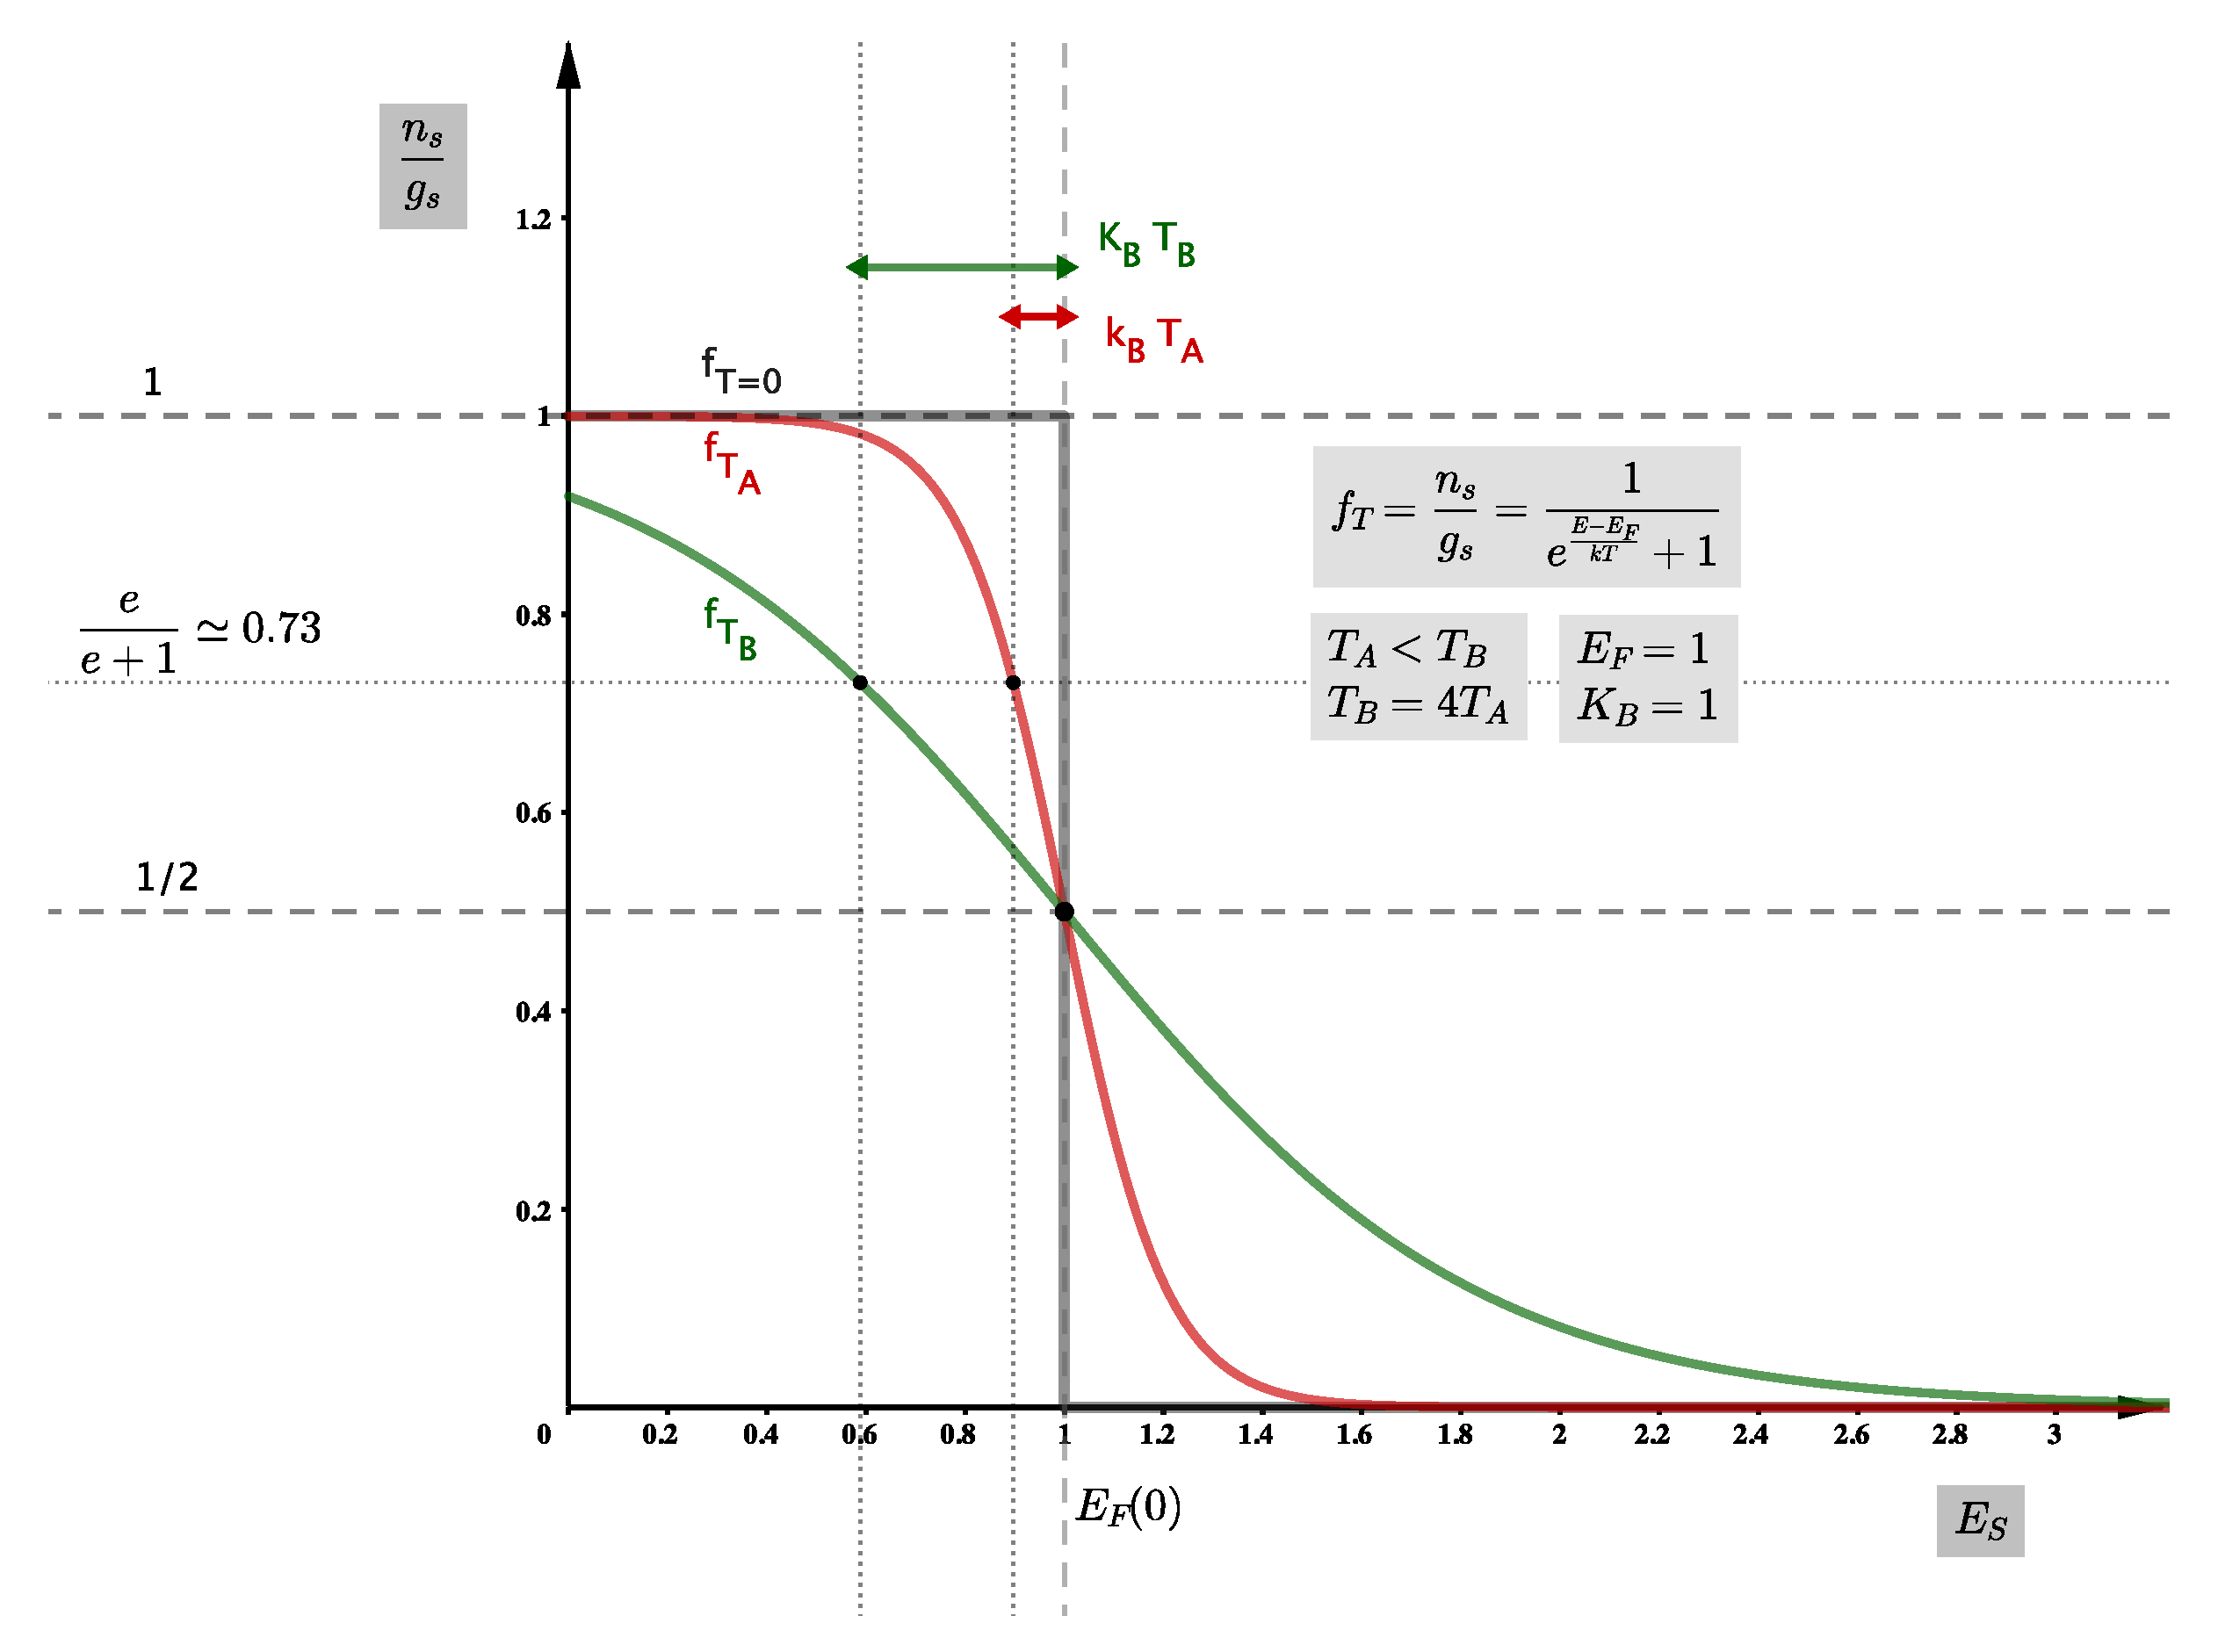
\includegraphics[scale=0.35]{/degenerazione3}
\caption{Nel grafico vengono riportate tre distribuzioni calcolate su tre temperature, nel testo: \quad
Caso a) funzione $f_{T_A}$
Caso b) funzione $f_{T_B}$
Caso c) funzione $f_{T=\SI{0}{K}}$
}
\label{degenerazione3}
\end{figure}


\subsection{Gas di elettroni}

Gli elettroni sono fermioni, la loro statistica è perciò descritta dal modello di Fermi-Dirac, poiché si tratta di particelle soggette al principio di esclusione di Pauli.
Gli \textbf{elettroni di conduzione nei metalli} sono un sistema quantistico anche a temperature \textit{normali} e non vicine allo zero assoluto, le densità tipiche di questi elettroni sono dell'ordine di $\SI{e28}{elettroni/m^3}$.

Quindi consideriamo un gas di elettroni, che seguono la statistica di Fermi Dirac, poiché fermioni, e si ha che la legge di distribuzione continua è la seguente, in cui compare $g(E)$ la \textit{funzione densità degli stati} (vedi \ref{fun_den_stat})
\begin{equation}
n(E)dE = \frac{ g(E)}{e^{ \frac{ E - E_F}{k_B T } } + 1 }
\quad\quad\quad\quad
g(E) = \frac{4 \pi V (2m^3)^{ \frac{1}{2} }}{h^3} E^{ \frac{1}{2} }
\end{equation}
trattandosi di elettroni, che hanno $spin=1/2$, gli stati disponibili raddoppiano e moltiplico x2, ottenendo
\begin{equation}
\begin{split}
n(E)dE & = 2 \cdot \frac{4 \pi V (2m^3)^{\frac{1}{2}} }{h^3} E^{\frac{1}{2}} \frac{1}{e^{\frac{E - E_F}{k_B T}} + 1} \\
& = \frac{8 \pi V (2m^3)^{\frac{1}{2}} E^{\frac{1}{2}}}{h^3} \frac{1}{e^{\frac{E - E_F}{k_B T}} + 1}
\label{nede_elet}
\end{split}
\end{equation}


\subsubsection{Cerco l'espressione generale del Livello di Fermi}
Calcolo il numero totale delle particelle nel sistema, integrando in $[0, \infty]$, vedi figura \ref{fig_integrali_a}
\begin{equation}
N = \int_0^{\infty} n(E)dE
\end{equation}
Se suppongo di essere alla temperatura dello \textit{zero assoluto} la temperatura è $T=\SI{0}{K}$ per cui la distribuzione è rappresentata dalla funzione a gradino ed allora ha senso calcolare l'integrale nell'intervallo $[0, E_F(0)]$ dove la distribuzione vale 1, oltre il valore $E_F(0)$ la distribuzione (il secondo fattore nella \ref{nede_elet}) vale 0.
Per una rappresentazione grafica vedi figura \ref{fig_integrali_b}.
Per cui equivale a calcolare il seguente integrale
\begin{equation}
\begin{split}
N & = \int_0^{E_F(0)} g(E)dE \\
& = \int_0^{E_F(0)} \frac{8 \pi V (2m^3)^{\frac{1}{2}} E^{\frac{1}{2}}}{h^3} dE \\
& = \frac{8 \pi V (2m^3)^{\frac{1}{2}}}{h^3} \int_0^{E_F(0)} E^{\frac{1}{2}} dE \\
& = \frac{16 \pi V (2m^3)^{\frac{1}{2}}}{3 h^3} E_F(0)^{\frac{3}{2}}
\label{num_parti_N}
\end{split}
\end{equation}
Da cui posso ricavare un'espressione per il \textit{Livello di Fermi}
\begin{equation}
\begin{split}
E_F(0) & = \frac{h^2}{8m}\Bigl(  \frac{3N}{\pi V}  \Bigr)^{ \frac{2}{3} } \\
& = \frac{h^2}{8m}\Bigl(  \frac{3}{\pi} n  \Bigr)^{ \frac{2}{3} } \\
& = \frac{h^2}{8m}\Bigl(  \frac{3}{\pi}  \Bigr)^{ \frac{2}{3} } n^{ \frac{2}{3} }
\end{split}
\end{equation}
in cui $n=\frac{N}{V}$ è una densità, infatti è definito come il numero di particelle sul volume, è importante notare che il Livello di Fermi dipende da $n^{ \frac{2}{3} }$ e quindi cresce al crescere della densità.


\subsubsection{Calcolo dell'energia totale del sistema}
È dato dall'integrale della funzione energia $E$ moltiplicata la distribuzione $n(E)$
\begin{equation}
U = \int_0^{\infty} E n(E) dE
\end{equation}
in cui è possibile utilizzare lo stesso ragionamento usato sopra ed integrare nell'intervallo $[0,E_F(0)]$
\begin{equation}
\begin{split}
U & = \int_0^{E_F(0)} E g(E) dE = \frac{8\pi V (2m^3)^{ \frac{1}{2} }}{h^3} \int_0^{E_F(0)} E^{ \frac{3}{2} } dE \\
& = \frac{2}{5} \frac{8\pi V (2m^3)^{ \frac{1}{2} }}{h^3} E_F(0)^{ \frac{5}{2} } = \frac{3}{5} N E_F(0) \\
& = \frac{3}{5} N \frac{h^2}{8m}\Bigl(  \frac{3}{\pi}  \Bigr)^{ \frac{2}{3} } n^{ \frac{2}{3} }
\end{split}
\end{equation}
dove l'ultimo passaggio è possibile considerando il risultato ottenuto nella \ref{num_parti_N} per $N$. \\
L'\textbf{energia media per particella} è data da
\begin{equation}
\frac{U}{N} = \frac{3}{5} E_F(0)
\end{equation}
Questo risultato è importante in quanto ci dice che anche alla temperatura dello zero assoluto, quindi a $T = \SI{0}{K}$ l'energia media è diversa da zero, cosa che non succede classicamente in cui l'energia media è $U = n K T$ per cui a $T=\SI{0}{K}$ sarebbe nulla.

\paragraph{Pressione di Pauli} Per la termodinamica: la pressione che un gas esercita sulla parete è pari a
\begin{equation}
P = \frac{2}{3} \frac{U}{V}
\end{equation}
che per un gas di elettroni diventa
\begin{equation}
P = \frac{2}{3} \frac{U}{V} = \frac{2}{3V} \frac{3}{5} N E_F(0) = \frac{2}{5} n E_F(0) 
\end{equation}
detta \textit{Pressione di Pauli}.
Anche allo zero assoluto esiste una pressione \textit{residua} del sistema.

\begin{figure}[h]
    \centering
    \subfloat[In \textit{verde}: l'integrale ad una temperatura $T$ generica]{
        \label{fig_integrali_a}
        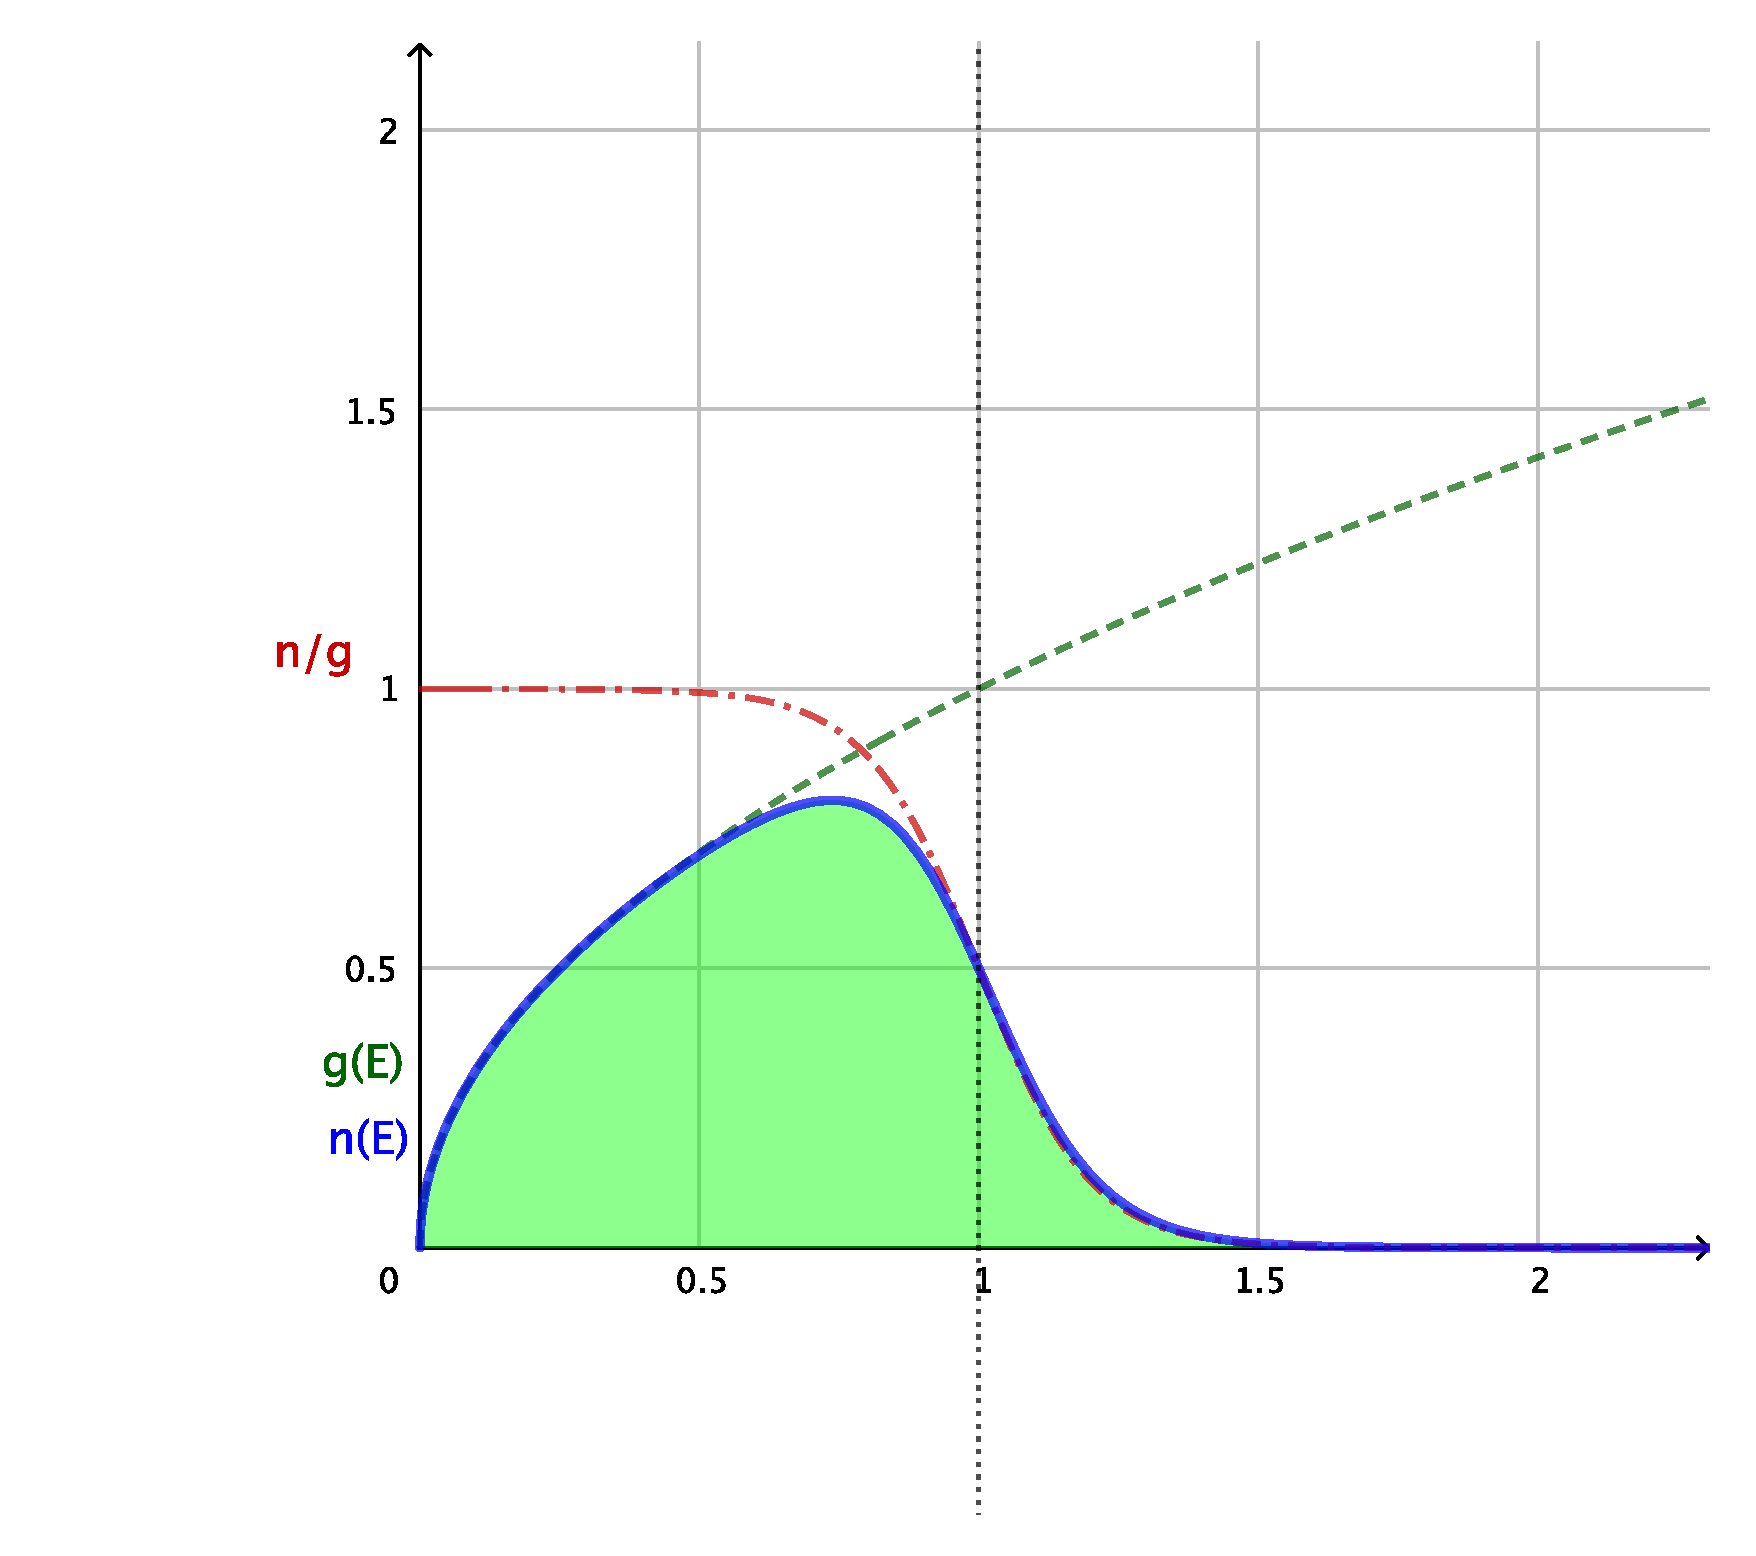
\includegraphics[ width=0.5\textwidth]{/integrale_1}
    }
    \subfloat[In \textit{blu}: l'integrale alla temperatura $T=\SI{0}{K}$]{
        \label{fig_integrali_b}
        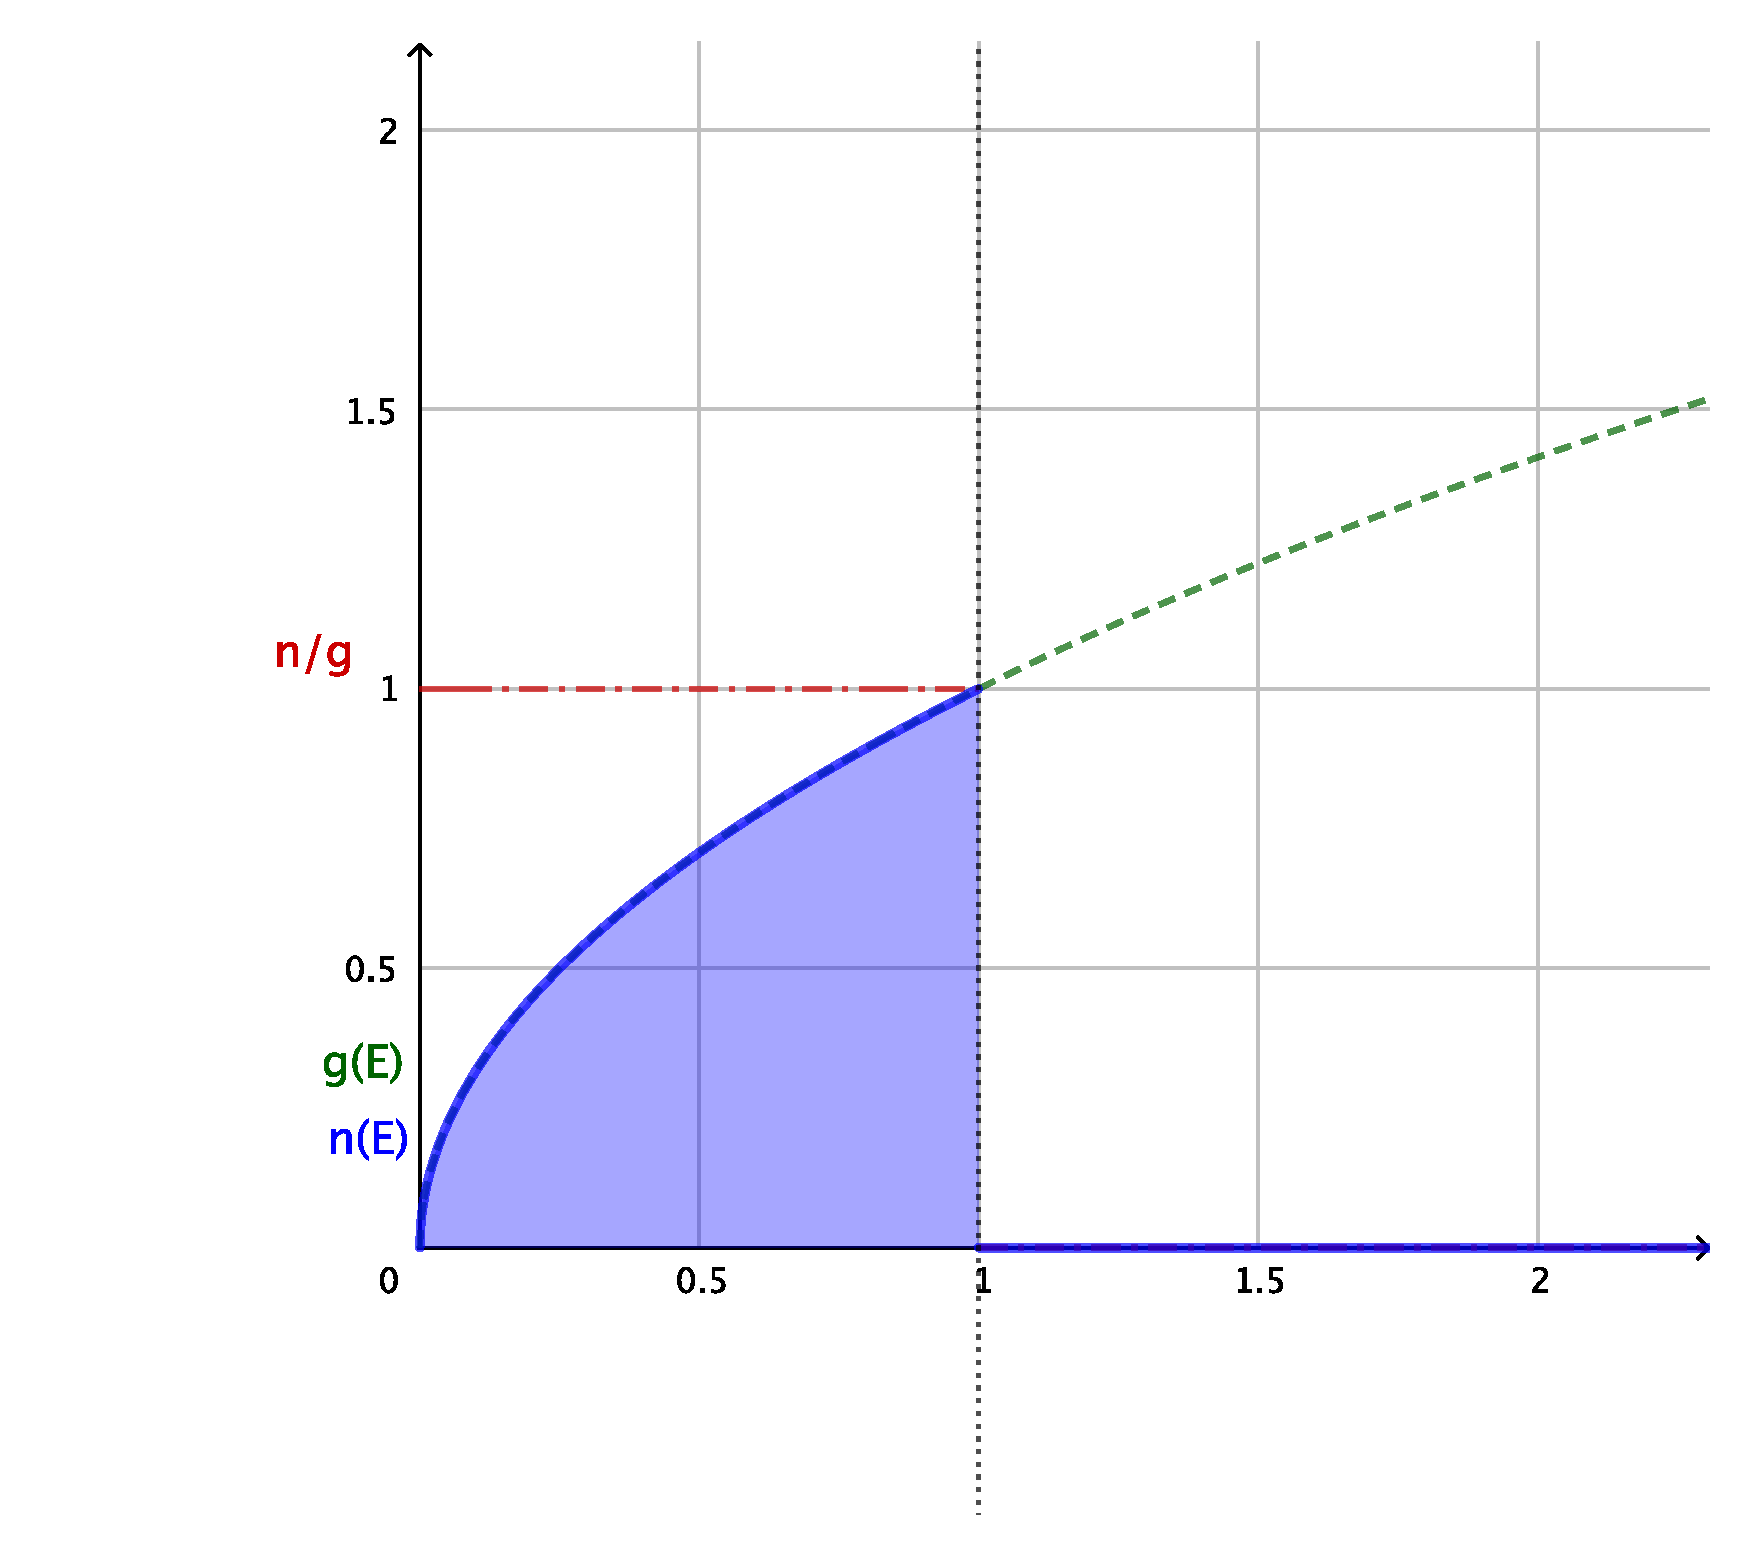
\includegraphics[ width=0.5\textwidth]{/integrale_2}
    }
    \caption{Gli integrali di questo capitolo vengono eseguiti a temperatura fissata $T=\SI{0}{K}$ per semplificare i conti, ciò è lecito poiché le due aree, \textit{verde} e \textit{blu} delle figure sopra, sono equivalenti.}
    \label{fig_integrali}
\end{figure}


\subsubsection{Calcolo della temperatura di Fermi $T_F$}
Nella teoria di Fermi Dirac, avendo fissato $\alpha$, ricavo il valore di $\xi$
\begin{equation}
\begin{split}
\alpha & = - \frac{E_F}{k_B T} \\
\xi & = e^{ -\alpha } = e^{ \frac{E_F}{k_B T} }
\end{split}
\end{equation}
se la temperatura è allo zero assoluto il parametro di degenerazione tende ad infinito per cui \textbf{il gas è totalmente degenere}
\begin{equation}
T=\SI{0}{K} \quad\Rightarrow\quad \xi \to + \infty
\end{equation}
le particelle sono "ammassate" nei livelli di più bassa energia, fino al Livello di Fermi.
Il gas rimane degenere fino a quando
\begin{equation}
k_B T \ll E_F(0) \quad\Rightarrow\quad T \ll T_F
\end{equation}
dove ribadiamo la Temperatura di Fermi \ref{temp_fermi}
$$T_F= \frac{E_F(0)}{k_B}$$
ovvero, per tali condizioni, si ha che l'Energia di Fermi $E_F$ coincide con il Livello di Fermi $E_F(0)$
\begin{equation}
\xi = e^{ \frac{E_F}{k_B T} } \simeq e^{ \frac{E_F(0)}{k_B T} } \gg 1
\end{equation}
Il gas non è degenere se
\begin{equation}
k_B T \gg E_F(0) \quad\Rightarrow\quad T \gg T_F
\end{equation}

\paragraph{Stima di $T_F$}
Supponiamo un metallo in cui ogni atomo fornisce un elettrone alla banda di conduzione, quindi un metallo con \textit{valenza} 1 (numero di elettroni fornito da ogni atomo).
La distanza tra gli elettroni sia circa
\begin{equation}
d \simeq \SI{0.1}{n m} = \SI{1}{\AA}
\end{equation}
la densità
\begin{equation}
n = \frac{1}{d^3}
\end{equation}
stimiamo la Temperatura di Fermi
\begin{equation}
T_F = \frac{E_F(0)}{k_B} = \frac{h^2}{8k_B m} \Bigl(  \frac{3}{\pi}  \Bigr)^{ \frac{2}{3} } n^{ \frac{2}{3} }
\end{equation}
considero che 
\begin{equation}
n^{ \frac{2}{3} } = \Bigl(  \frac{1}{d^3}  \Bigr)^{ \frac{2}{3} } = d^{ -2 }
\end{equation}
allora la Temperatura di Fermi risulta
\begin{equation}
\begin{split}
T_F & = \frac{E_F(0)}{k_B} = \frac{h^2}{8k_B m} \Bigl(  \frac{3}{\pi}  \Bigr)^{ \frac{2}{3} } d^{ -2 } \\
& = \Bigl(\frac{3}{\pi}\Bigr)^{\frac{2}{3}}\frac{6.6^2}{8 \cdot 1.38 \cdot 9.1 \cdot 1} 
\cdot \frac{10^{-68}}{10^{-23}10^{-31}10^{-20}} \frac{\SI{}{J^2.s^2}}{\SI{}{\frac{J}{K}.Kg.m^2}} \\
& = \SI{4.20e5}{K}
\end{split}
\end{equation}
La temperatura di Fermi stabilisce il confine che separa il regime in cui vale la statistica classica $(T>T_F)$ da quello in cui vale la statistica quantistica $(T<T_F)$, quindi per un gas di elettroni a temperature \textit{ordinarie} sono sempre in un regime degenere.


\subsubsection{Calore specifico elettronico}
Si definisce \textbf{calore specifico molare} il calore necessario per innalzare di un grado la temperatura di una mole di una sostanza
\begin{equation}
c_V = \frac{dU}{dT}
\end{equation}
l'energia totale è 
\begin{equation}
U = \frac{3}{2}N k_B T
\end{equation}
quindi classicamente otterrei
\begin{equation}
c_V =  \frac{dU}{dT} = \frac{3}{2} N k_B
\end{equation}

Cerco il calore specifico di un gas di elettroni a volume costante, quindi non essendo banale calcolarlo, applico una approssimazione: ipotizzo di essere ad una temperatura diversa dallo zero assoluto ma di poco più alta per cui vale la relazione
$$k_B T \ll E_F(0)$$
allora la differenza tra questo caso ed il caso allo zero assoluto differisce di una frazione delle $N$ particelle (elettroni) data da 
\begin{equation}
N \Bigl(  \frac{k_B T}{E_F(0)}  \Bigr)
\end{equation}
che aumenta la sua energia di un ordine di $k_BT$.
Per cui c'è un aumento totale dell'energia del sistema di
\begin{equation}
\Delta U \simeq N \Bigl(  \frac{k_B T}{E_F(0)}  \Bigr) \cdot k_B T
\end{equation}
dove compare il numero delle particelle moltiplicato l'energia. \\
Allora il calore specifico è dato da
\begin{equation}
c_V =  \frac{dU}{dT} \simeq N k_B \Bigl(  \frac{T}{T_F}  \Bigr)
\end{equation}
Con un calcolo più preciso si trova la seguente relazione, che differisce solo di un fattore numerico
\begin{equation}
c_V = \frac{\pi^2}{2} N k_B \Bigl(  \frac{T}{T_F}  \Bigr)
\end{equation}
da cui si vede che solo al di sopra della temperatura di Fermi si trova il risultato classico.

\paragraph{Buca di potenziale}
La descrizione di pareti di potenziale infinite non è realistica, ciò che si ha è che gli elettroni possono uscire da una buca di potenziale, a patto che si possa fornirgli energia sufficiente.

\begin{figure}[h]
\centering
\includegraphics[scale=0.8]{/buca_poten_calspec}
\caption{Buca di potenziale di un metallo}
\end{figure}

Questo spiega l'\textbf{effetto termoionico}: è un fenomeno per cui un metallo riscaldato ad una temperatura sufficientemente alta inizia ad emettere elettroni presenti sulla sua superficie. 
A $T \not= \SI{0}{K} $ gli elettroni cominciano ad occupare gli strati più elevati e ad uscire dalla buca di potenziale.
Per i metalli, la funzione lavoro ed il livello di Fermi sono dell'ordine degli $\SI{}{eV}$.

\begin{figure}[h]
\centering
\includegraphics[scale=1]{/metalli_energia_estrazione_livello_Fermi}
\caption{Funzione lavoro e livello di Fermi di alcuni metalli}
\end{figure}








 

    %%
%% Author: dariochinelli
%% 2021-04-06
%%


\section{Calore specifico di un solido cristallino}
È stato un problema della fisica affrontato da molti studiosi, come Einstein e Debye, nel corso dei primi del '900, che ha aperto una nuova visione su vari ambiti.
il calore specifico molare a volume costante è definito come
\begin{equation}
c_V = \frac{1}{N} \frac{dU}{dT}
\end{equation}
dove $N$ rappresenta il numero di moli.
Questa grandezza misura l'energia necessaria per far variare di un grado la temperatura di una mole di sostanza.
Un cristallo è una struttura geometrica in cui gli atomi occupano posizioni ben precise.
Quindi studiamo il calore specifico di un reticolo tridimensionale di atomi.
In Fisica classica il calore specifico di un solido è lo stesso per tutti i materiali, in una mole ci sono $N_A$ atomi ed ognuno di questi atomi può eseguire oscillazioni armoniche semplici attorno alla posizione di equilibrio, da cui si scrive l'energia totale considerando le tre dimensioni come
\begin{equation}
U = 3 N_A k_B T = 3 R T
\end{equation}
in cui ogni oscillatore armonico ha una energia media $k_B T$, come calcolato anche grazie alla statistica classica di Maxwell Boltzmann nei capitoli precedenti, 
ed in cui $R$ è la costante universale dei gas.
Eseguendo la derivata ottengo la \textbf{legge classica di Dulong Petit (1819)}
\begin{equation}
c_V = \frac{dU}{dT} = 3 R = \SI{6}{cal / mol . K}
\end{equation}
Dai dati sperimentali si osserva che al diminuire della temperatura il calore specifico ha una dipendenza dalla temperatura e non è più costante, la legge di Dulong Petit è valida quindi solo sopra la \textit{temperatura ambiente}.
Vicino allo zero assoluto e a basse temperature si ha un andamento del tipo
\begin{equation}
c_V \propto T^3
\end{equation}
Per i metalli al di sotto di temperature di $\SI{10}{K}$ si torna ad avere un andamento lineare. \\


\subsection{Modello di Einstein}
Einstein propose un modello teorico che fosse più consistente con l'evidenza sperimentale.
Egli ritenne che ad ogni mole di sostanza non si dovesse associare un'energia $kT$ bensì un termine che tenesse conto della quantizzazione, esattamente come fece Planck per il Corpo Nero, Einstein considerò che ogni mole di sostanza avesse un'energia data dal termine
\begin{equation}
k_B T \quad\Rightarrow\quad \frac{ h \nu}{e^{ \frac{ h\nu}{k T } } - 1 }
\end{equation}
per cui l'energia totale diventa
\begin{equation}
\begin{split}
U & = 3 N_A \frac{h \nu}{e^{ \frac{h\nu}{k_B T} } - 1} \\
& = 3 R T \frac{\frac{h\nu}{k_B T}}{e^{ \frac{h\nu}{k_B T} } - 1}
\end{split}
\end{equation}
implicando che il sistema sia un insieme di $3 N_A$ oscillatori armonici semplici, aventi tutti la \underline{stessa frequenza} di oscillazione.
Usando $\beta = \frac{1}{k_B T}$ si trova
\begin{equation}
c_V = \frac{dU}{dT} = \frac{3N_A (h\nu)^2}{k_B T^2} \frac{e^{ \beta h \nu }}{(e^{ \beta h \nu }-1)^2}
\end{equation}

\paragraph{Ad alte temperature} per $\beta h \nu \to 0$ e quindi per $\frac{h\nu}{k_B T} \to 0$ si può sviluppare in serie l'esponenziale
\begin{equation}
e^{ \beta h \nu } = 1 + \beta h \nu ...
\end{equation}
e trovare l'energia
\begin{equation}
U = \frac{ 3 N_A h \nu}{\beta h \nu } = 3 N_A k T = 3 R T
\end{equation}
ed il calore specifico 
\begin{equation}
c_V = 3 N_A k_B
\end{equation}
ritrovando la formula di Dulong Petit per $k_B T \gg h \nu$.

\paragraph{A basse temperature} il calore specifico $c_V$ diminuisce, in particolare si ha una diminuzione importante per $k_B T\le h \nu$ ed ancora più determinante quando $k_B T \ll h \nu$ per cui:
\begin{equation}
\begin{split}
& T\to0 \quad\Rightarrow\quad \beta \to \infty \\
c_V & = \frac{3 N_A (h\nu)^2}{k_B T^2} \frac{e^{\beta h \nu}}{(e^{\beta h \nu}-1)^2} \\
& = \frac{3 N_A (h\nu)^2}{k_B T^2} \frac{e^{\beta h \nu}}{e^{2 \beta h \nu}} = \frac{3 N_A (h\nu)^2}{k_B T^2} e^{- \beta h \nu} \\
& = \frac{3 N_A (h\nu)^2}{k_B} \frac{e^{- \frac{h \nu}{k_B T}}}{T^2}
\end{split}
\end{equation}
che tende a zero come $T^2$.
Il modello di Einstein fu un notevole passo avanti, ma rimaneva ancora un problema: a basse energie, l'andamento non si adattava come $T^3$ del calore specifico.

\begin{figure}[h]
\centering
\includegraphics[scale=0.5]{/calore_specifico_energia}
\caption{Andamento del calore specifico e dell'energia, teoria di Einstein. Tutte le costanti nel grafico sono poste unitarie.}
\end{figure}


\subsection{Modello di Debye}
Ciò è da ricondurre ad un errore nelle assunzioni di Einstein: 
non c'era alcun motivo per cui le frequenze degli oscillatori armonici dovessero essere le stesse, 
questo avrebbe implicato l'esistenza di una frequenza caratteristica diversa per ogni materiale, ipotesi priva di fondamento.
A risolvere questi interrogativi fu Debye col suo modello nel 1912.
L'intuizione di Debye fu assumere che gli atomi che compongono un sistema cristallino non vibrino in modo indipendente l'uno dall'altro e che al contrario la vibrazione di ciascun atomo \underline{dipenda} dagli altri.
Si parla quindi di \underline{catena unidimensionale di atomi} accoppiati da \textit{forze armoniche}.
Per cui considero un sistema di $N_A$ atomi e di $3 N_A$ modi di vibrazione, ognuno avente una propria frequenza $\nu$, problema risolvibile con la fisica classica.

Per trovare lo \textit{spettro di frequenze} di vibrazione assume che il solido si comporti come un mezzo continuo tridimensionale, e non come un sistema discreto di atomi.
Considera allora solo modi di vibrazione longitudinali con nodi al bordo.
Il calcolo dello spettro di frequenze risulta essere identico a quello svolto per le onde elettromagnetiche dentro la cavità di corpo nero, a meno del fattore 2 dei due possibili stati di polarizzazione e della sostituzione della velocità della luce $c$ con la velocità $v$ di propagazione dell'onda nel mezzo
\begin{equation}
N(\nu)d\nu = 2 \frac{ 4 \pi V}{c^3 } \nu^2 d\nu \quad\Rightarrow\quad N(\nu)d\nu = \frac{ 4 \pi V}{v^3 } \nu^2 d\nu
\end{equation}
Si deve imporre un vincolo: il numero di modi di vibrazione possibili è fissato al valore $3 N_A$, per cui
\begin{equation}
\int_0^{\nu_m} N(\nu)d\nu = 3 N_A 
\end{equation}
quindi esiste una frequenza massima $\nu_m$, per considerare il fatto che il sistema sia discreto e non continuo, per il quale la frequenza massima sarebbe infinita.
Svolgendo l'integrale si ottiene
\begin{equation}
\frac{4\pi V}{3 v^3} \nu_m^3 = 3 N_A 
\quad\Rightarrow\quad
\nu_m = v \Bigl(  \frac{9 N_A}{4 \pi V}  \Bigr)^{ \frac{1}{3} }
\end{equation}
espressione della frequenza massima, frequenza di "taglio". \\
Se ogni modo di vibrazione è trattato come un oscillatore armonico unidimensionale di energia media data dalla relazione di Planck
\begin{equation}
\bar\varepsilon = \frac{h\nu}{e^{ \frac{h\nu}{k_B T} } - 1}
\end{equation}
coincide a trattare il sistema con la statistica classica di Boltzmann: gli atomi sono distinguibili nel reticolo del cristallo, ottengo quindi
\begin{equation}
\begin{split}
U = \int_0^{\nu_m} \bar\varepsilon \cdot N^omodi  
& = \int_0^{\nu_m}  \frac{h\nu}{e^{ \frac{h\nu}{k_B T} } - 1} \cdot \frac{4\pi V}{v^3} \nu^2 d\nu \\
& = \frac{9 N_A h}{\nu_m^3} \int_0^{\nu_m} \frac{\nu^3}{e^{ \frac{h\nu}{k_B T} } - 1}
\end{split}
\label{energia_tot_debye_1}
\end{equation}
in cui ho sostituito 
$$\frac{4\pi V}{v^3} = \frac{9 N_A }{\nu_m^3}$$
Dalla \ref{energia_tot_debye_1}, imponendo le seguenti sostituzioni 
\begin{equation}
\begin{split}
& x = \frac{h\nu}{k_B T} \quad\quad\quad d\nu = \frac{k_B T}{h} dx \\
& x_m = \frac{h}{k_B T} \nu_m \quad\quad \nu_m = \frac{k_B T}{h} x_m \quad\quad k_B N_A = R
\label{sostituzioni}
\end{split}
\end{equation}
trovo un'altra forma dell'energia totale di Debye, più consona per svolgere i conti seguenti
\begin{equation}
U = 3 R T \frac{3}{x_m^3} \int_0^{x_m}  \frac{x^3 dx}{e^x-1}
\label{energia_tot_debye_2}
\end{equation}

\paragraph{Temperatura di Debye}
Osservando che la quantità $h \nu_m / k_B$ ha le dimensioni di una temperatura, si definisce allora la \textbf{Temperatura di Debye} come
\begin{equation}
\Theta = \frac{h \nu_m}{k_B} = \frac{h}{k_B} \Bigl(  \frac{9 N_A}{4 \pi V}  \Bigr)^{ \frac{1}{3} } v
\label{temp_debye}
\end{equation}
Nel particolare la temperatura di Debye rappresenta la temperatura alla quale sono "attivati" tutti i modi possibili di oscillazione degli oscillatori armonici che compongono il materiale, fino al livello massimo $\nu_m$.
La temperatura di Debye è una caratteristica di ogni sostanza, vediamone alcune nella tabella seguente
\begin{table}[h]
\centering
\begin{tabular}{lll}
\hline
\textbf{Elemento} \quad\quad & \textbf{$\Theta$  $[K]$} \quad\quad & \textbf{$\nu_m$  $[10^{12} s^{-1}]$} \\ \hline
Diamante & 1860 & 38.8 \\
Ferro & 465 & 9.7 \\
Alluminio & 395 & 8.3 \\
Argento & 210 & 4.4 \\
Elio solido & 30 & 0.6 \\ \hline
\end{tabular}
\caption{Temperatura di Debye e frequenza massima per alcuni elementi}
\end{table}

\paragraph{Calcolo dell'energia totale}
Il limite superiore di integrazione risulta essere
$$x_m = \frac{\Theta}{T}$$
e l'energia media di Debye si può scrivere come
\begin{equation}
U = 9 R \frac{T^4}{\Theta^3} \int_0^{\Theta/T}  \frac{x^3 dx}{e^x-1}
\label{energia_tot_debye_3}
\end{equation}
Considerando ora che $c_V$ è la derivata dell'energia totale $U$ nella temperatura $T$, ponendo le sostituzioni \ref{sostituzioni} e inserendo la temperatura di Debye \ref{temp_debye} otteniamo la \textbf{formula di Debye per il calore specifico}
\begin{equation}
\begin{split}
c_V = \frac{dU}{dT} & = \frac{9 N_A h^2}{\nu_m^3 k_B T^2} \int_0^{\nu_m}\frac{\nu^4 e^{ \frac{h\nu}{k_BT} }}{\Bigl(  e^{ \frac{h\nu}{k_BT} }-1  \Bigr)^2} d\nu \\
& = 9 R \Bigl(  \frac{T }{\Theta}  \Bigr)^3 \int_0^{\Theta/T} \frac{x^4 e^x}{(e^x - 1)^2} dx
\end{split}
\end{equation}
Per procedere nel calcolo dell'energia e del calore specifico si distinguono due condizioni:

\begin{itemize}
\item Nel caso di \textbf{basse temperature}, per $T \to 0 \quad\Rightarrow\quad  \frac{\Theta}{T} \to \infty$, vediamo che il limite superiore di integrazione tende ad infinito, risultato valido per temperature molto inferiori alla temperatura di Debye, quindi per
$$T \ll \Theta \quad\quad\quad\quad k_B T \ll h \nu_m$$
per cui
\begin{equation}
U = 9R \frac{T^4}{\Theta^3} \int_0^{\infty} \frac{x^3}{e^x-1} dx
= \frac{3}{5} \pi^4 R \Bigl(  \frac{T^4}{\Theta^3}  \Bigr)
\end{equation}
in cui l'integrale noto vale
$$\int_0^{\infty} \frac{x^3}{e^x-1} dx = \frac{\pi^4}{15}$$
Per il calore specifico
\begin{equation}
c_V = \frac{dU}{dT} = \frac{12}{5} \pi^4 R \Bigl(  \frac{T}{\Theta}  \Bigr)^3
\end{equation}
trovo l'andamento $T^3$ compatibile con i risultati sperimentali.

\item Nel caso di \textbf{alte temperature}, per $T \to \infty \quad\Rightarrow\quad \frac{\Theta}{T} \to 0$, per cui la variabile di integrazione è compresa in un intervallo tra 0 ed un numero che tende a zero, questo risultato è valido per temperature molto maggiori alla temperatura di Debye, quindi per
$$T \gg \Theta \quad\quad\quad\quad k_B T \gg h \nu_m$$
per cui posso sviluppare in serie di Taylor $ e^x \sim 1 + x + ... $
\begin{equation}
\begin{split}
U & = 9R \frac{T^4}{\Theta^3} \int_0^{\Theta/T} \frac{x^3}{e^x-1} dx
= 9R \frac{T^4}{\Theta^3} \int_0^{\Theta/T} x^2 dx \\
& = 9R \frac{T^4}{\Theta^3} \cdot \frac{\Theta^3}{3 T^3}
= 3 R T
\end{split}
\end{equation}
ritrovando la legge di Dulong Petit e quindi che il calore specifico ad alte temperature è costante e vale
\begin{equation}
c_V = 3R
\end{equation}
\end{itemize}

\paragraph{Conclusioni} sulla legge di Debye si vede un grande accordo tra la teoria ed i dati sperimentali, riportiamo in figura \ref{dabye_datispe} un grafico che evidenzia questo fatto
\begin{figure}[h]
\centering
\includegraphics[scale=0.8]{/modello_debye_dati_sperimentali}
\caption{Il modello di Debye rapportato ai dati sperimentali}
\label{dabye_datispe}
\end{figure}


\subsection{Il calore specifico in un metallo vicino allo zero assoluto}
Se considero un metallo ad una temperatura $T$ molto bassa vicino allo zero assoluto, oltre al contributo reticolare (visto sopra) ho anche un contributo dato dagli elettroni che lo compongono (visto nei capitoli precedenti), per cui
\begin{equation}
\begin{split}
c_{V reticolare} & = \frac{12}{5} \pi^4 R \Bigl(  \frac{T}{\Theta}  \Bigr)^3 \\
c_{V elettronico} & = \frac{\pi^2}{2} N k_B \frac{T}{T_F}
\end{split}
\end{equation}
nella prima vale ovviamente la relazione $k_B N_A = R$ costante dei gas e nella seconda $N$ equivale al numero di elettroni del sistema e $T_F$ è la temperatura di Fermi.
Notiamo che per il contributo reticolare c'è una dipendenza $T^3$ mentre per il contributo elettronico c'è dipendenza lineare in $T$.

Possiamo stimare la temperatura alla quale il contributo reticolare domina sul contributo elettronico, facciamo quindi il rapporto tra il calore specifico elettronico ed il calore specifico reticolare
\begin{equation}
\begin{split}
\frac{c_{V elettronico} }{c_{V reticolare} } & = \frac{\pi^2}{2} N k_B \frac{T}{T_F} \frac{5}{12} \frac{1}{\pi^4 R} \frac{\Theta^3}{T^3} \\
& = \frac{5}{24 \pi^2} \frac{N k_B}{R} \frac{\Theta^3}{T_F T^2}
= \frac{5}{24 \pi^2} \frac{N}{N_A} \frac{\Theta^3}{T_F T^2} 
\end{split}
\label{rapp_cv_elet_reti}
\end{equation}
Il rapporto $\frac{N}{N_A}$ corrisponde alla \textit{valenza}, cioè quanti elettroni per ogni atomo vengono dati in banda di conduzione, quindi quanti elettroni per atomo formano il \textit{gas di elettroni}. \\
Imponendo il rapporto \ref{rapp_cv_elet_reti} uguale a 1, trovo la temperatura critica oltre la quale il contributo reticolare supera quello elettronico
\begin{equation}
\begin{split}
\frac{c_{V elettronico} }{c_{V reticolare} } = 1
\quad\Rightarrow\quad 
T_0 = \Bigl(  \frac{5}{24 \pi^2} \frac{N}{N_A} \frac{\Theta^3}{T_F} \Bigr)^\frac{1}{2}
\simeq \Bigl(  \frac{\Theta}{T_F}  \Bigr)^\frac{1}{2} \Theta
\end{split}
\end{equation}
la temperatura $T_0$ è una frazione della temperatura di Debye, quindi risulta essere dell'ordine di qualche grado Kelvin.



    
    %%
%% Author: dariochinelli
%% 2021-04-07
%%


\section{Catena unidimensionale di atomi (\textit{dinamica fononica})}
Per questo studio considero una catena unidimensionale, che non è il problema più generale in tre dimensioni da poter risolvere ma generalizza meglio il problema visto nel capitolo precedente sullo studio approssimato di Debye. \\

% ------- ------- ------- ------- ------- ------- ------- ------- ------- ------- -------
Un mezzo solido continuo supporta sia vibrazioni longitudinali sia trasversali, ma Debye ha agito nel modo seguente:
\begin{equation}
\int_0^{\nu_m} N(\nu) d\nu = 3 N_A \Rightarrow \frac{ 4\pi V}{v^3 } \nu_m^3 = 3 N_A
\end{equation}
Ma nel caso più corretto possibile, il solido in questione, soffre di oscillazioni sia trasversali che longitudinali.
Occorre dunque dividere la velocità dell'onda nelle sue componenti.
\begin{equation}
3N_A = \frac{ 3 \pi V}{3 } \nu_m^3 \Bigl(  \frac{ 1}{v_l^3 } + \frac{ 2}{v_t^3 }  \Bigr) \quad\quad \mbox{dove si è usato} \quad
\frac{ 1}{v^3 } = \Bigl(  \frac{ 1}{v_l^3 } + \frac{ 2}{v_t^3 }  \Bigr)
\end{equation}
Dove il 2 sta ad indicare che le onde trasversali hanno due possibili stati di polarizzazione, mentre ce n'è uno solo per le onde longitudinali,
e dunque ciò che abbiamo visto finora vale solo nel caso in cui le onde sono tutte longitudinali, ma ciò non è sempre vero. \\
% ------- ------- ------- ------- ------- ------- ------- ------- ------- ------- -------

Consideriamo quindi una catena unidimensionale di atomi chiusa su se stessa, a \textit{collana}, e detta condizione al contorno di Born–von Karman e cerco di calcolare il numero di modi di vibrazione.
Introduciamo la seguente nomenclatura:
\begin{equation}
\begin{split}
x_n & = \mbox{ posizione $n$-esima particella} \\
R_n & = \mbox{ posizione di equilibrio $n$-esima particella} \\
u_n & = (x_n - R_n) = \mbox{ spostamento dalla posizione di equilibrio } \\
a & = \mbox{ distanza reticolare, distanza fra due posizioni di equilibrio} \\
K & = \mbox{ costante elastica delle molle} \\
\end{split}
\end{equation}
\begin{figure}[h]
\centering
\includegraphics[scale=0.2]{/catena_unidim_atomi}
\caption{Catena unidimensionale di atomi}
\end{figure}
Poiché la catena è chiusa, si impongono condizioni al contorno periodiche.
La forza di interazione tra due particelle è nulla quando la molla è all'equilibrio e cioè quando $x_2-x_1 = a$, quando si trovano ad una distanza $a$, quindi la forza $F_{21}$ che agisce sulla particella $2$ a causa della connessione con $1$
\begin{equation}
\begin{split}
F_{21} & = - K (x_2 - x_1 - a) \\
& = - K (x_2 - R_2 - x_1 + R_1 + R_2 - R_1 - a) \\
& = - K (u_2 - u_1)
\end{split}
\label{forza_F21}
\end{equation}
L'equazione del moto è data da due termini: uno ricavato sopra \ref{forza_F21} ed uno analogo tra la particella $2$ e la particella $3$
\begin{equation}
m \ddot{x_2} = - K (u_2 - u_1) + K (u_3 - u_2)
\end{equation}
la somma è dovuta al fatto che quando la quantità al secondo membro è positiva, l'interazione spinge la particella verso destra sull'asse $x$.
Le derivate seconde $\ddot{x_2} = \ddot{u_2}$ sono equivalenti, per cui è dunque possibile scrivere l'equazione del moto generica per l'$n$-esima particella, 
(sulla quale però si approssima valutando solo le interazioni fra le particelle adiacenti)
\begin{equation}
\begin{split}
m \ddot{u_n} & = - K (u_n - u_{n-1}) + K (u_{n+1} - u_n) \\
& = K \Bigl[  u_{n-1} + u_{n+1} - 2 u_n  \Bigr]
\label{eqmoto_nesimapart}
\end{split}
\end{equation}
La soluzione di questa equazione può essere espressa come onda longitudinale \textit{viaggiante} del tipo
\begin{equation}
u_n = s e^{ i k R_n } e^{ - i \omega t } = s e^{ i (k n a - \omega t) }
\label{solution_un}
\end{equation}
dove
\begin{equation}
\begin{split}
k = \frac{2\pi}{\lambda} \quad \mbox{numero d'onda} \quad\quad&\quad\quad s  = \quad \mbox{ampiezza} \\
\omega = 2 \pi \nu  \quad \mbox{frequenza} \quad\quad\quad\quad&\quad\quad R_n = n a \\
\end{split}
\end{equation}
Sostituendo la soluzione \ref{solution_un} nell'equazione differenziale \ref{eqmoto_nesimapart} dopo aver trovato la derivata 
\begin{equation}
\frac{d^2}{dt^2} u_n = \ddot{u_n} = -\omega^2 s e^{ i ( k n a - \omega t ) }
\end{equation}
ottengo
\begin{equation}
\begin{split}
- \omega^2 m s e^{ i (k n a - \omega t) } & = K \Bigl(  s e^{ - i \omega t }  \Bigr) \Bigl[  e^{ i k (n-1) } + e^{ i k (n+1) } - 2 e^{ i k n } \Bigr] \\
- \omega^2 m s e^{ i k n a } & = K \Bigl[  e^{ - i k a } + e^{ i k a } - 2 \Bigr] e^{ i k n a } \\
\omega^2 m  & = K ( 2 - 2 \cos (k a) )
\end{split}
\end{equation}
utilizzo l'identità trigonometrica: $\sin^2 \frac{ X}{2 } = \frac{ 1}{2 } \Bigl(   1 - \cos(X)  \Bigr)$
\begin{equation}
\omega^2 = \frac{4 K}{m} \sin^2 \frac{k a}{2} 
\quad\Rightarrow\quad 
\omega = 2 \sqrt{\frac{K}{m}} \Bigl| \sin \frac{ka}{2}  \Bigr| \quad\quad\quad \mbox{(da ricordare)}
\label{omega}
\end{equation}
questa formula collega insieme la frequenza $\omega$ ed il numero d'onda $k$.

\paragraph{Studio la funzione in base al valore di $k$} 
Per piccoli numeri d'onda $k$, cioè per grandi lunghezze d'onda $\lambda$, posso approssimare la \ref{omega} con
\begin{equation}
\omega = 2 \sqrt{\frac{K}{m}} \Bigl| \frac{ka}{2}  \Bigr|  \quad\Rightarrow\quad \omega \propto k
\end{equation}
per cui la \textit{velocità di fase}
\begin{equation}
v_{fase} = \frac{\omega}{k}
\end{equation}
è uguale alla \textit{velocità di gruppo}
\begin{equation}
v_{gruppo} = \frac{d \omega}{d k}
\end{equation}
da cui trovo che è indipendente dalla frequenza e vale
\begin{equation}
\frac{\omega}{k} = c = \frac{d \omega}{d k} = \sqrt{\frac{K}{m} a^2}
\end{equation}
allora si dice che \textit{non c'è dispersione}.

Per valori qualsiasi di $k$, uso la \ref{omega} e trovo la funzione $\sin$, periodica su un periodo $2\pi / a$.
La funzione \ref{omega} nell'intervallo $\Bigl[  -\frac{\pi}{a}, +\frac{\pi}{a}  \Bigr]$, detta \textit{"1st Brillouin Zone"}, plottata permette di capire meglio il concetto di dispersione, vedi figura \ref{dispersione} \\
\begin{figure}[h]
\centering
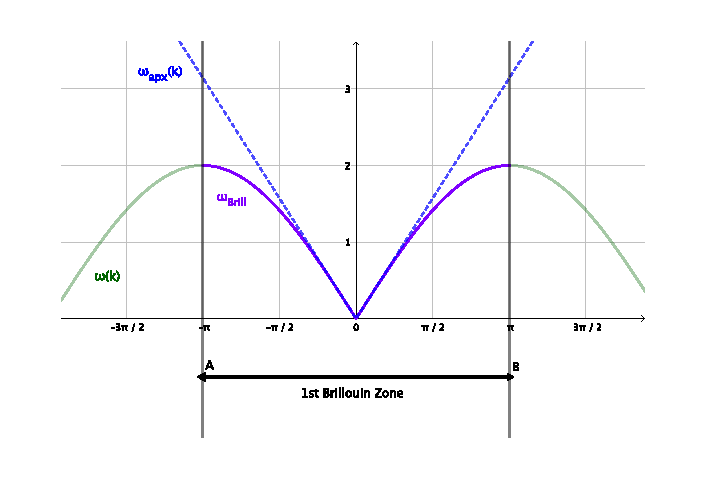
\includegraphics[scale=0.8]{/brillouinzone}
\caption{Curva di dispersione, zona di Brillouin}
\label{dispersione}
\end{figure}
Il distacco tra la funzione lineare e la funzione seno è dovuto al fatto che non ho a che fare con un sistema continuo ma discreto.
Per piccoli $k$ per cui le due curve combaciano, non ho dispersione, mentre per $k$ più grandi le due curve si allontanano e ho dispersione.
Cioè aumentando $k$ non è più vero che la velocità non dipende dalla frequenza e quindi avrò onde a diverse velocità, quindi dispersione.

\paragraph{Condizioni su $k$} avendo considerato una catena di atomi circolare, si dovrà imporre l'uguaglianza tra la funzione relativa al primo atomo e quella relativa all'atomo $N+1$ ovvero
\begin{equation}
\begin{split}
u_1 &= u_{N+1} \\
s \Bigl(  e^{ ika } e^{ -i \omega t }  \Bigr) & =  s \Bigl(  e^{ ik(N+1)a } e^{ -i \omega t }  \Bigr) = s \Bigl(  e^{ ika } e^{ ikNa } e^{ -i \omega t }  \Bigr)
\end{split}
\end{equation}
vera se soddisfa la condizione 
\begin{equation}
e^{ ikNa } = 1
\end{equation}
ovvero
\begin{equation}
k = \frac{2\pi}{N a} l \quad\quad\quad \mbox{quindi} \quad -\frac{N}{2} < l \le \frac{N}{2}
\end{equation}
quindi se $k$ varia di una quantità $\frac{2\pi}{a}$ allora $u_n$ non cambia;
ci sono allora solo $N$ valori di $k$ consistenti con la condizione scritta sopra.


\subsection{Fononi}
In alternativa alla trattazione del capitolo precedente, posso ragionare in termini di particelle per cui ho un modo di frequenza $\omega(k)$ con energia
\begin{equation}
\varepsilon = n h \nu = n \hbar \omega
\end{equation}
e considerare lo stato che contiene $n$ particelle con energia $\hbar \omega$ e numero d'onda $k$
\begin{equation}
\bar \varepsilon = \frac{h \nu}{e^{ \frac{h\nu}{k_B T} } - 1}  
= \frac{\hbar \omega}{e^{ \frac{\hbar\omega}{k_B T} } - 1}  
\end{equation}
tali particelle sono dette \textit{fononi}, descrivibili come i quanti di energia elastica (meccanica), collegata ai moti di vibrazione reticolare.
Sono definite come particelle a \textit{massa nulla} e \textit{spin zero}, sono quindi descrivibili come \textit{bosoni}.
Si può vedere come l'analogo di un fotone: quanto di energia elettromagnetica, ma relativo alle onde elastiche. \\
Utilizzando i \textit{fononi} è possibile trattare alcuni fenomeni di fisica classica e dello stato solido come ad esempio:
\begin{itemize}
\item il calore specifico
\item la resistenza elettrica
\item la trasmissione del calore attraverso un metallo
\item la misura di diffrazione neutronica
\end{itemize}





    
    %%
%% Author: dariochinelli
%% 2021-04-08
%%


\section{Applicazione della statistica di Bose-Einstein}


\subsection{Gas di fotoni e corpo nero}
Oltre alla possibilità di utilizzare la statistica di Maxwell-Boltzmann per risolvere il problema del Corpo Nero, come affrontato nei primi capitoli, un altro modo di risolvere il problema è considerare che la luce, nella cavità di Corpo Nero, sia un \textit{gas di fotoni}: particelle con massa nulla e spin unitario.
Considerando i fotoni come \textit{bosoni}, i quali non sono soggetti al Principio di Esclusione di Pauli, e quindi tendono ad accumularsi nel livello energetico più basso, il livello fondamentale $E=0$, avente energia minore.
Occorre usare la statistica di Bose-Einstein, che scritta nel modo generico con $\beta = 1/ k_B T$ risulta essere
\begin{equation}
\begin{split}
& \frac{ n_s}{g_s } = \frac{ 1}{e^{ \alpha + \beta E_s } - 1 } = \frac{ 1}{e^{ \alpha} e^{ E / k_B T } - 1 } \\
\quad\Rightarrow\quad & n(E)dE = g(E) \frac{ 1}{e^{ \alpha} e^{ E / k_B T } - 1 } dE
\end{split}
\end{equation}
Nel caso di fotoni il numero di particelle nel sistema $N$ \textit{non è costante}, per cui il moltiplicatore di Lagrange associato è
\begin{equation}
\alpha = 0 \quad\Rightarrow\quad e^{\alpha} = 1 \quad\Rightarrow\quad  \xi = 1
\end{equation}
all'interno della cavità di Corpo Nero c'è uno scambio continuo fra il campo di radiazione e le pareti della cavità, per cui i fotoni vengono assorbiti ed emessi continuamente.
Dato che il parametro di degenerazione è pari a 1, non è certamente $\ll 1$ e dunque \emph{un gas di fotoni in equilibrio con la materia è sempre degenere}.
Quindi la legge di distribuzione dei fotoni è
\begin{equation}
n(E)dE = g(E) \frac{1}{e^{ E / k_B T } - 1 } dE
\end{equation}
L'energia di un fotone è pari a $E = h \nu$ la moltiplico per la distribuzione di Bose Einstein per ottenere la \textit{densità di energia}
\begin{equation}
\varrho_T(\nu) d\nu = \frac{h\nu n(\nu)d\nu}{V}
\label{dens_ener}
\end{equation}
Quindi esplicitando la distribuzione di Bose Einstein in funzione della frequenza si trova
\begin{equation}
n(\nu)d\nu = g(\nu) \frac{1}{e^{ h\nu / k_B T } - 1 } d\nu
\end{equation}
in cui $g(\nu)$ deriva dallo studio della funzione densità degli stati $g(E)$ da cui si ottiene quella in funzione della frequenza
\begin{equation}
\begin{split}
g(E) & = \frac{dN}{dE} = \frac{4 \pi V (2m^3)^{ \frac{1}{2} }}{h^3} E^{ \frac{1}{2} } \quad\quad \mbox{eq \ref{dens_stati}} \\
& E = \frac{p^2}{2m} \quad\Rightarrow\quad dN = g(p)dp = g(E)dE \\
g(p) & = g(E) \frac{dE}{dp} = \frac{4\pi V}{h^3} p^2 \\
& p = \frac{h}{\lambda} = \frac{h \nu}{c} \quad\Rightarrow\quad  g(\nu)d\nu  = g(p)dp \\
g(\nu) & = g(p) \frac{dp}{d\nu} = 2 \cdot \frac{4\pi V}{h^3} \nu^2
\end{split}
\end{equation}
il fattore 2 deriva dal considerare le due orientazioni possibili dello spin del fotone.
Utilizzando le espressioni ricavate sopra
\begin{equation}
n(\nu)d\nu = g(\nu) \frac{1}{e^{ h\nu / k_B T } - 1 } d\nu 
\quad\quad\quad\quad
g(\nu) = \frac{8\pi V}{h^3} \nu^2
\end{equation}
riscriviamo allora la funzione densità di energia
\begin{equation}
\varrho_T(\nu) d\nu = \frac{8 \pi \nu^2}{c^3} \cdot \frac{h\nu}{e^{\frac{h\nu}{k_B T}} - 1} d\nu
\end{equation}
che corrisponde alla \textit{Formula di Planck per il corpo nero}.


\subsection{Gas di fononi}
Un ragionamento analogo al precedente ci permette di ottenere una relazione per i fononi.
L'energia del fonone di tipo $\textbf{k}$ della branca $s$ è
\begin{equation}
E = \hbar \omega_s (\textbf{k})
\end{equation}
e l'energia totale sarà la prima delle seguenti
\begin{equation}
\begin{split}
E & = \sum_{\textbf{k}_s} \frac{\hbar \omega_s(\textbf{k})}{e^{ \hbar \omega_s (\textbf{k}) / k_B T } - 1} \\
E & = \sum_{\textbf{k}_s} \hbar \omega_s(\textbf{k}) \Bigl(  \frac{1}{e^{ \hbar \omega_s (\textbf{k}) / k_B T } - 1} + \frac{1}{2}  \Bigr)
\end{split}
\end{equation}
mentre la seconda corregge l'approssimazione fatta per l'energia dell'oscillatore armonico...
per cui considera anche l'\textit{energia di punto zero}.
Si trova allora il calore specifico, derivando la somma sulle branche dell'integrale sulla prima zona di Brillouin
\begin{equation}
c_V = \frac{\partial}{\partial T} \sum_{s} \int 
\frac{d \textbf{k}}{(2\pi)^3} 
\frac{\hbar \omega_s(\textbf{k})}{e^{ \hbar \omega_s (\textbf{k}) / k_B T } - 1}
\end{equation}
eseguendo questo conto per basse temperature posso assumere $\hbar \omega_s \textbf{k} \gg k_B T$
e considero i modi con $\omega_s \textbf{k}$ piccolo $(\textbf{k} \to 0)$ e $\omega = c k$, integrando su tutto lo spazio $k$,
trovo l'\textbf{approssimazione di Debye}
\begin{equation}
\begin{split}
& \mbox{con} \quad\quad x = \frac{\hbar c_s k}{k_B T} \quad\quad d\textbf{k} = k^2 dk 4\pi \\
c_V & \propto \frac{\partial}{\partial T} \Bigl(  3 T^4 \int_0^{\infty} \frac{x^3}{e^x - 1} dx  \Bigr) \approx T^3
\end{split}
\end{equation}


\subsection{Condensazione di Bose-Einstein}
Considero un gas di bosoni, la statistica che lo regola è 
\begin{equation}
\frac{n_s}{g_s} = \frac{1}{e^{ \alpha + \beta E_s } - 1}
\end{equation}
ed imponendo che i parametri di Lagrange siano
\begin{equation}
\beta = \frac{1}{k_B T} \quad\quad\quad \alpha > 0
\end{equation}
trovo che a temperatura $T = \SI{0}{K}$ solo gli stati con $E_s = 0$ sono occupati, assumendo $g_0  = 1$ trovo
\begin{equation}
N \simeq \frac{ 1}{e^{ \alpha } - 1 }
\label{N_alpha}
\end{equation}
ed invertendo trovo la relazione
\begin{equation}
e^{\alpha} = 1 + \frac{1}{N} \simeq 1 \quad \mbox{quando } N \to \infty
\end{equation}
per cui il sistema è degenere.
Essendo $\alpha \to 0$ posso sviluppare la \ref{N_alpha} come
\begin{equation}
N \simeq \frac{1}{1+ \alpha - 1} = \frac{1}{\alpha}
\end{equation}
lasciando esplicito $g_0$ avrei
\begin{equation}
n_0 \simeq N \simeq \frac{g_0}{e^{ \alpha } - 1 }
\quad\quad
e^{\alpha} = 1 + \frac{g_0}{N} \simeq 1
\quad\quad
N \simeq \frac{g_0}{\alpha}
\end{equation}

La relazione 
\begin{equation}
e^{\alpha} \simeq 1
\end{equation}
resta valida anche a $T \not= 0$ vicina allo zero assoluto, per cui posso chiedermi quante particelle sono all'energia \emph{ground state} $E_s = 0$?
Cerco un'espressione per $n_0$, il ground state, in funzione della temperatura
\begin{equation}
N = \sum_s n_s = n_0 (T) + n_e(T)
\end{equation}
ovvero la somma tra il numero di particelle nello stato fondamentale più il numero di particelle in tutti gli altri stati, stati eccitati.
Utilizzo l'equazione al continuo per la legge di Bose Einstein e la funzione densità degli stati 
\begin{equation}
\begin{split}
n(E)dE & = g(E) \frac{ 1}{e^{ \alpha + E / k_B T } - 1 } dE \\
g(E)dE & = \frac{4\pi V (2m^3)^{ \frac{1}{2} }}{h^3} E^{ \frac{1}{2} } dE
\end{split}
\end{equation}
e quindi integro nell'intervallo $\Bigl[  0, \infty  \Bigr]$
\begin{equation}
\begin{split}
N & = n_0 + \int_0^{\infty} n(E)dE \\
& = n_0 + c \int_0^{\infty} \frac{E^{ \frac{1}{2} }}{e^{ \alpha + \beta E } - 1} dE
\end{split}
\end{equation}
in cui ho sostituito e sostituisco
\begin{equation}
\begin{split}
& c = \frac{4\pi V (2m^3)^{ \frac{1}{2} }}{h^3} \\
& z= \beta E \quad\quad\quad dE = \frac{dz}{\beta} = dz k_B T
\end{split}
\end{equation}
e ottengo
\begin{equation}
N = n_0 + c(k_B T)^{\frac{3}{2}} G(\alpha)
\label{N_di_gamma}
\end{equation}
definendo la funzione \emph{gamma}
\begin{equation}
G(\alpha) = \int_0^{\infty} x^{ \frac{1}{2} } (e^{ z + \alpha } - 1) dz
\end{equation}
Se $\alpha$ è grande
\begin{equation}
\begin{split}
G(\alpha) & = e^{ - \alpha} \int_0^{\infty} x^{ \frac{1}{2} } e^{ -z } dz \\
G(\alpha) & \to e^{-\alpha} \frac{\sqrt{\pi}}{2}
\end{split}
\end{equation}
Se $\alpha$ è piccolo
\begin{equation}
\begin{split}
& G(0) \to 2.612 \frac{\sqrt{\pi}}{2} \\
& \alpha \simeq \frac{1}{N} \to 0 \quad\Rightarrow\quad G(\alpha) \approx G(0)
\end{split}
\end{equation}
allora l'equazione \ref{N_di_gamma} diventa
\begin{equation}
\begin{split}
N = n_0 + c (k_B T)^{ \frac{3}{2} } G(\alpha)
\quad\Rightarrow\quad 
n_0 & = N -  c (k_B T)^{ \frac{3}{2} } G(0) \\
& = N -  c (k_B T)^{ \frac{3}{2} } 2.612 \frac{\sqrt{\pi}}{2}
\end{split}
\end{equation}

Dalla formula 
\begin{equation}
\frac{n_0}{N} = 1 - \Bigl(  \frac{T}{T_C}  \Bigr)^{ \frac{3}{2} } 
\label{n0N}
\end{equation}
crivo la temperatura critica come
\begin{equation}
\begin{split}
T_C & = \frac{1}{k_B} \Bigl(  \frac{2N}{c \sqrt{\pi} 2.612}  \Bigr)^{ \frac{3}{2} } \\
&= \frac{2\pi \hbar^2}{k_B m} \Bigl(  \frac{N/V}{2.612}  \Bigr)^{ \frac{3}{2} } \propto \rho^{ \frac{3}{2} }
\end{split}
\end{equation}
quindi la temperatura critica è proporzionale alla densità elevata alla due terzi,
Plottando la relazione \ref{n0N} di $\frac{n_0}{N}$ si trova 
%% PLOT
Dalla temperatura critica $T_C$ diminuendo la temperatura tutte le particelle iniziano ad affollare lo stato fondamentale.
Che coincide alla \emph{condensazione di Bose Einstein}: tutte le particelle occupano lo stato fondamentale.







	\newpage

\begin{figure}[h]
\centering
\includegraphics[scale=0.25]{/andamenti_Cv_T}
\end{figure}
Il numero di particelle nello stato fondamentale rimane grande fino a che $T < T_c$.
Al di sotto della temperatura critica le particelle sono condensate nel livello energetico minore di energia, cioè si ha il fenomeno della \underline{condensazione di Bose-Einstein}.
\begin{equation}
C_V = N K \Bigl(  \frac{ T}{T_c }  \Bigr) C \quad \mbox{dove} \quad C \to 1.9
\end{equation} 

Un fenomeno affascinante, affine alla condensazione di Bose-Einstein, è la superconduttività dell'elio liquido, per cui si consiglia di leggere il seguente paragrafo:

\textit{"Bose Condensation and liquid helium", pag 399-404, da Eisnerg-Resnick, Quantum Physics of atoms, molecules, solids, nuclei and particles}.







    
%    %%
%% Author: dariochinelli
%% 2021-04-10
%%


\section{Reticoli cristallini}








    
% \fi
\end{document}



